\documentclass[a4paper,12pt,twoside,openright]{report}
\usepackage[titletoc]{appendix}
\usepackage{textcomp}
\usepackage[pdftex]{color,graphics}
\usepackage{amssymb}
\usepackage{verbatim}
\usepackage{graphicx}
\usepackage{graphics}
\usepackage{amsmath}
\usepackage{rotating}
\usepackage{setspace}
\usepackage{multirow}
\usepackage{array}
\usepackage{hhline}
\usepackage[labelfont={bf}, margin=0.5cm]{caption}
\usepackage{pdflscape}
\usepackage{subcaption}
\usepackage{caption}
\usepackage{xspace}
\usepackage{float}
\usepackage{placeins}
\usepackage{etoolbox}
\usepackage{xkeyval}[2006/11/18]
\usepackage{datetime}
\usepackage[a4paper,inner=2.5cm,outer=1.5cm,top=2.5cm,bottom=2.5cm,pdftex]{geometry}
\usepackage{emptypage}
\usepackage{hyperref}
\usepackage{titlesec}

\hypersetup{
	linktocpage,
    colorlinks = true,
	linkcolor = blue,
	citecolor = red
}

\usepackage{fancyhdr}
\fancyfoot{}
\pagestyle{fancy}
\fancyhead[LO]{\leftmark}
\fancyhead[RE]{\rightmark}
\fancyhead[RO,LE]{\thepage}

\renewcommand{\textfraction}{.05}
\renewcommand{\floatpagefraction}{.40}

\newcommand{\gr}{$\gamma$-ray\xspace}
\newcommand{\grs}{$\gamma$-rays\xspace}

\usepackage{lipsum}% just to automatically generate text

\makeatletter
\newcommand\ackname{Acknowledgements}
\if@titlepage
  \newenvironment{acknowledgements}{%
      \titlepage
      \null\vfil
      \@beginparpenalty\@lowpenalty
      \begin{center}%
        \bfseries \ackname
        \@endparpenalty\@M
      \end{center}}%
     {\par\vfil\null\endtitlepage}
\else
  \newenvironment{acknowledgements}{%
      \if@twocolumn
        \section*{\abstractname}%
      \else
        \small
        \begin{center}%
          {\bfseries \ackname\vspace{-.5em}\vspace{\z@}}%
        \end{center}%
        \quotation
      \fi}
      {\if@twocolumn\else\endquotation\fi}
\fi
\makeatother

\newdateformat{monthyeardate}{%
  \monthname[\THEMONTH], \THEYEAR}

%\textheight 24cm
%\textwidth 16.5cm
%\topmargin -1cm
%\oddsidemargin  0cm
%\evensidemargin 0cm
%\flushbottom

%\usepackage{etoolbox}
%\patchcmd{\chapter}{\thispagestyle{plain}}{\thispagestyle{fancy}}{}{}

\setlength{\headheight}{15pt}


\begin{document}


\setcounter{secnumdepth}{3}
\setcounter{tocdepth}{3}

%\doublespace

\pagenumbering{roman}

\begin{titlepage}

\begin{center}

\textbf{\Huge Upgrades to the }

\vspace{3mm}

\textbf{\Huge Fluorescence Detectors of the}

\vspace{3mm}

\textbf{\Huge Pierre Auger Observatory} 

\vspace{3cm}


\includegraphics[width=0.3\textwidth]{pix/UoA_col_vert.png}

\vspace{3cm}


\textbf{\large Tristan William Sudholz} \\
\vspace{0.4cm}
\large School of Physical Sciences \\
\vspace{0.1cm}
\large University of Adelaide

\vspace{1.5cm}
\large This dissertation is submitted for the degree of \\
\vspace{0.2cm}
\textit{\large Doctor of Philosophy}
\vspace{2.5cm}

\monthyeardate\today

\end{center}

\end{titlepage}

\chapter*{Declaration}

I, Tristan William Sudholz, certify that this work contains no material which has been accepted for the award of any other 
degree or diploma in any university or other tertiary institution and, to the best of my knowledge and
belief, contains no material previously published or written by another person, except where due
reference has been made in the text. In addition, I certify that no part of this work will, in the future,
be used in a submission for any other degree or diploma in any university or other tertiary institution 
without the prior approval of the University of Adelaide and where applicable, any partner institution
responsible for the joint-award of this degree.

I give consent to this copy of my thesis, when deposited in the University Library, being made
available for loan and photocopying, subject to the provisions of the Copyright Act 1968.

I also give permission for the digital version of my thesis to be made available on the web, via the
University’s digital research repository, the Library catalogue and also through web search engines,
unless permission has been granted by the University to restrict access for a period of time. 

\vspace{2cm}

\line(1,0){150}

\vspace{1cm}

Tristan William Sudholz
\chapter*{Abstract}


%
\chapter*{Acknowledgements}



\tableofcontents
%\listoffigures
%\listoftables

\chapter*{Nomenclature}

\addcontentsline{toc}{chapter}{Nomenclature}

\begin{tabular}{p{8em} p{30em}}
PAO & Pierre Auger Observatory \\
EAS & Extensive Air Shower \\
NSB & Night Sky Background \\
PE & Photo-electron \\
FD & Fluorescence Detector \\
SD & Surface Detector \\
PMT & Photomultiplier Tube \\
FLT & First Level Trigger
\end{tabular}

% Background Chapters

\chapter*{Introduction}\label{Ch:Intro}
\markright{Introduction}
\addcontentsline{toc}{chapter}{Introduction}
\pagenumbering{arabic}

\begin{itemize}
\item Define Cosmics Rays.
\item The origins of the highest energy cosmic-rays still unknown.
\item First detection by Pierre Auger in 1937 and the current detector looking at theses energies is the Pierre Auger Observatory.
\item Hybrid experiment containing both surface detectors and fluorescence detectors
\item Surface detector has nearly 100\% up-time while the fluorescence detectors only have 15\% up-time.
\item **** Proposal to extend the fluorescence detector up-time. To achieve this will have to operator while the moon is above the horizon. This will increase the level NSB and will have the PMTs run under a reduced gain to compensate. ****
\item Photomultiplier Tubes are used as pixels within the camera of the fluorescence detectors and  the aim of these thesis is to quantify the characteristics of the PMT under the reduced gain and increased.
\item Outline a Summary of each chapter.
\end{itemize}


Cosmic-rays are particles that originate outside of the Earth atmosphere. These particles can be photons, hadronic or leptonic in nature [ref?]. In this thesis, when mentioning cosmic-rays I will mean the hadronic component unless specified otherwise. Cosmic-rays have been measurement over a large range of energies (over 6 decades in energy) and it has many interesting features have been observed in this energy spectrum. One of the longest running mysteries is what happens at the highest energy. Since the first detection of extensive air showers by Pierre Auger in 1937 [ref], many different experiments have endeavoured to solve this mystery. The Pierre Auger Observatory [ref] is currently in operation to observe cosmic-rays at the highest energies. 

The Pierre Auger Observatory is a hybrid experiment consisting of both surface detectors and fluorescence detectors. (Outline location) The surface detector has a nearly 100\% operation up-time {ref} while the fluorescence detectors only 15\% operation up-time [ref]. (Outline how PAO detects cosmic-rays, just need a brief summary).

A current proposal to extend the fluorescence detector operation up-time. Extended up-time would be beneficial as the fluorescence detectors image the entire extensive air shower and would increase the number of showers observed through out yearly observation. To achieve the extended operation the fluorescence detectors would have to operated while the moon is above the horizon. While the moon is up, this would increased the Night Sky Background level and to compensate the Photomultiplier Tubes acting as the camera pixels would have to be run under reduced gain. 

The aim of this thesis is to quantify the characteristics of the Photomultiplier Tubes operating under this reduced gain and outline any operation strategies. Outline of each chapter is as follows:

\begin{itemize}
\item  Chapter \ref{Ch:Cosmic-rays}: Cosmic-rays

Does this work as a new line

\item Chapter \ref{Ch:CR_Detection}: Detection of Cosmic-Rays

Add text here

\item Chapter \ref{Ch:PAO}: The Pierre Auger Observatory

Add text here

\item Chapter \ref{Ch:SelectEff} : EAS Selection Efficiency with Increased NSB 

Add text here

\item Chapter \ref{Ch:PMTCharacter} : Quantifying Characteristics of the FD PMT 

Add text here

\item Chapter \ref{Ch:CompSimPMT} : Computer Simulation of the FD PMT 

Add text here

\item Chapter \ref{Ch:GainVariance} : Measuring Gain Variance of the FD PMT with CalA data 

Add text here

\item Chapter \ref{Ch:LabPMTshift} : Laboratory Simulation of FD Shifts

Add text here

\item Chapter \ref{Ch:CloudCuts} : Effectiveness of Cloud Camera Cuts

Add text here

\item Chapter \ref{Ch:Conclusion}: Conclusion 

Future Work


\end{itemize}
\chapter[Cosmic-Rays]{\centering Cosmic-Rays \\}\label{Ch:Cosmic-rays}

\section{History of Cosmic-Rays}

First detection of ionizing radiation. 

1785: Coulomb found that 
electroscopes can spontaneously 
discharge by the action of the air 
and not by defective insulation

1835: Faraday confirms the 
observation by Coulomb, with 
better insulation technology

1879: Crookes measures that the 
speed of discharge of an 
electroscope decreased when 
pressure was reduced 

\section{Energy Spectrum and Mass composition}

\begin{figure}[hp]
\centering
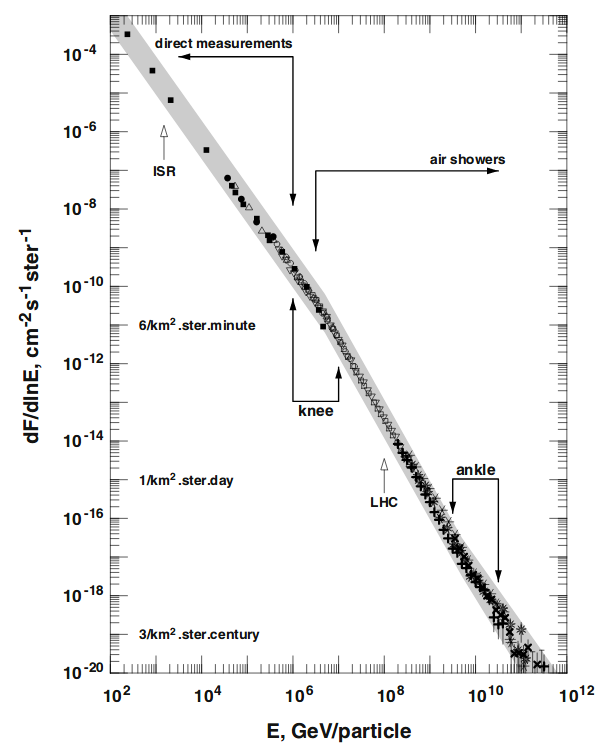
\includegraphics[width=\textwidth]{chapters/pix/CosmicRay_Spectrum.png}
\caption{Measured energy spectrum of cosmic-rays from 100 GeV up to the highest detected energy.}
\label{fig:CR_Spectrum}
\end{figure}

Cosmic-rays have been detected over a large range of energies from GeV (10$^9$ \ eV) to above EeV (10$^18$ \ eV). Spectrum in Figure \ref{fig:CR_Spectrum} shows the break at the knee and ankle and which type of experiments are most suited to measurement each part. Cosmic-ray spectrum starts out at E$^{-2}$ \ and can be as steep as E$^{-2.7}$ at the highest energies.

Cosmic-rays can consist of protons to iron. 

\section{Production Method and Sources}

Supernova explosions 

AGN jets

other energetic processes

dark matter annihilations.
\chapter{Detections of Cosmic-Rays}\label{Ch:CR_Detection}

\section{Extensive Air Showers}

Use Earth's atmosphere as an interaction medium.
Primary particle interacts with the molecules in the atmosphere to produce a cascade of secondary particles. This cascade of particles is referred to as an Extensive Air Shower (EAS).
Hadronic primaries can produce pions, muons and other stuff.
Mixture of a hadronic core with an electromagnetic component from the decay of $\pi^{0}$.

Shower profile has particles produced until energy on individual secondary particles drop below the ionization threshold. Therefore the shower will reach a point of maximum particle number then will drop off.

\section{Fluorescence Production}

The charge particles of EAS interact with the nitrogen molecules in the atmosphere. This interaction turns the nitrogen molecule dipole like and when the nitrogen returns to a ground state, a photon is emitted. This emitted photon is termed fluorescence light. Fluorescence light is can be emitted isotropically and typically in the UV band (between 300 and 400 nm). *** Show wavelength profile ***


\section{Atmospheric Effects}




\section{Detectors and History}

Early Experiments:

Volcano Ranch

Haverah Park

SUGAR

Yakutsk array is located in Russia and has been operating in different forms since 1967. The array reached a maximum collecting area of 17 km$^2$ around 1990. Recently it has been reconfigured to have a collection area of 8 km$^2$ to study lower energy cosmic-rays.

Akeno Gaint Air Shower Array (AGASA) is located in Tokyo, Japan. Operating at an average altitude of 667 m above sea level from 1990 to 2004. The array consist of over one hundred scintillator detectors covering 100 km$^2$ ***check this***. The timing measurements and data collection is achieved via interconnected optical fibers.

The Fly's Eye was the first successful air fluorescence detector operating from 1981 to 1993 at the Dugway Proving Grounds in Utah, USA. Fly's Eye achieved a time averaged aperture of about 100 km$^2$sr at the highest energies, considering it only operated on clear moonless nights. 

HiRes improved on the Fly's Eye design by advancing resolution and sensitivity, This was achieved by increasing the telescope effective mirror area to 3.8 m$^2$ and reducing the camera pixel angular diameter to 1\textdegree. 
\chapter{Pierre Auger Observatory}\label{Ch:PAO}


Science Goals

Location

\section{Hybrid Detector}

\subsection{Surface Detector}

\subsection{Fluorescence Detector}

\section{Communication System and CDAS}

\section{Event Reconstruction}

\subsection{Surface Detector}

\subsection{Fluorescence Detector}

\section{Enhancements and future upgrades}

% Result Chapters

\chapter[EAS Selection Efficiency with Increased NSB]{\centering Extensive Air Shower Selection Efficiency with Increased \\ Night Sky Background \\}\label{Ch:SelectEff}


%Selection Efficiency of EAS under increased NSB
%\begin{itemize}
%\item Smearing real data with extra noise
%\item Simulating EAS with an increased NSB
%\item Talk about differences in smearing and simulating EAS (different triggering conditions)
%\item Energy and Xmas resolution and bias
%\item Rp bias
%\item differences in track length
%\end{itemize}

\section{Motivation}

The FD shifts are typically organised for night with the illuminated fraction of the moon less then 70\% and can be operated longer than 3 hours of moon below the horizon. The Fd telescope shutters are then opened when the sun is below -18\textdegree of the horizon (astronomical twilight), the average variance of the camera PMTs less then 100 ADC$^2$ and individual PMTs less then 2000 ADC$^2$. Two calculations where done by the collaboration to estimate the theoretical up time of the FD's. Before 2012 the theoretical calculations looked like:

\begin{table}[h]
\centering
\begin{tabular}{c c}
Theoretical up time & 22\% \\
Loss due to short nights ($<$ 3 hrs) & -2\% \\
Loss due to bad weather or fails & -5\% \\ \hline \hline
Total measurement time & 15\% 
\end{tabular}
\end{table}

For context the measured ADC$^2$ for typically observed Night Sky Background (NSB) with no moon, quarter moon and full moon/twilight is:
\begin{table}[h]
\centering
\begin{tabular}{c c c}
\hline\hline
Condition & $\sigma^2$ [ADC$^2$] & I$_{\mathrm{a}}$ [$\mu$A] \\ \hline\hline
no moon & 25 & 0.5 \\
quarter moon & 250 & 5 \\
full moon/twilight & 2500 & 50 \\ \hline\hline
\end{tabular}
\end{table}

These values are measured under the standard operation of the FD's. Further within this thesis I will investigate lower the gain on the PMTs to reduce the variance and current that their under. A lower current when observing under moonlight would help make sure that the PMT lifespans are not changed by the increased in NSB.

The signal that the FD's observe is AC coupled, which means the mean signal of the NSB is zero. Instead the variance around zero is calculated andis directly proportional to the fluctuations in the NSB. The average value of the NSB measured by POA at Malargue is:
\begin{equation}
\sigma^2 \sim 25 \ \mathrm{ADC}^2
\end{equation}
The variance in ADC$^2$ can be converted into photons seen at the aperture by using:
\begin{eqnarray}
\sigma^2_{pe} &=& [\sigma^2_{\mathrm{ADC}}]^{\mathrm{sky}} \ / \ \mathrm{A}^2_{\mathrm{G}} \label{eq:simgaPE} \\
\mathrm{n}_{\mathrm{ph}} &=& \frac{\sigma^2_{pe}}{(1 + \mathrm{V}_{\mathrm{G}})} \label{eq:numPhoton}
\end{eqnarray}
where $\sigma_{pe}$ is the standard deviation of the photo-electron count, n$_{\mathrm{ph}}$ is the photon count and A$_{\mathrm{G}}$ is equal to:
\begin{equation}\label{eq:abs_gain}
\mathrm{A}_{\mathrm{G}} = \frac{1}{\mathrm{C}_{\mathrm{FD}}.\mathrm{f}.\mathrm{Q}}
\end{equation}
where
\begin{itemize}
\item[] A$_{\mathrm{G}}$ is the absolute gain (ADC/photo-electron)
\item[] $\mathrm{C}_{\mathrm{FD}}$ is the FD pixel calibration constant.
\item[] Q is the Quantum efficiency of the PMT.
\item[] f is the efficiency if the telescope optics.
\end{itemize}

/*------ \textbf{Find reference to number below} ------*/

Assuming typical measured values for C$_{\mathrm{FD}}$, Q and f shown in:
\begin{table}[h]
\begin{center}
\begin{tabular}{|c|c|}
\hline
C$_{\mathrm{FD}}$ & 4.5 photons/ADC \\
\hline
Q & 0.29 \\
\hline
f & 0.465 \\
\hline
\end{tabular} 
\end{center}
\caption{} 
\end{table} \label{tab:CFD_Q_F}

Therefore A$_{\mathrm{G}}$ can be calculated from Eq. \ref{eq:abs_gain} and using the values from Table \ref{tab:CFD_Q_F}. If $\sigma^2_{\mathrm{ADC}}$ = 25 ADC$^2$, through the calculations n$_{\mathrm{ph}}$ = 23 photons / 100 ns. The calculations to work out the RMS$_{\mathrm{ph}}$ from the measured variance in ADC$^2$ is as follows:
\begin{equation}
\mathrm{RMS}_{\mathrm{ph}} = \mathrm{C}_{\mathrm{FD}} \times \sqrt{\mathrm{ADC}^2}
\end{equation}
From all of the equations stated above I have outlined a table showing the expected photon count at the aperture per 100 ns from the measured variance (ADC$^2$ / 100 ns).
\begin{center}
\begin{tabular}{| c | c | c | c |}
\hline \hline
\textbf{Variance} & \multirow{2}{*}{\textbf{log$_{10}$(V/ADC$^2$)}} & \multirow{2}{*}{\textbf{Photons/100 ns}} & \textbf{RMS} \\
\textbf{(ADC$^2$ / 100 ns)} & & & \textbf{(Photons/100 ns)} \\
\hline \hline
25 & 1.40 & 22.7 & 22.5 \\
\hline
178 & 2.25 & 161.4 & 60 \\
\hline
259 & 2.40 & 226.7 & 71.2 \\
\hline
1000 & 3.00 & 907.0 & 142.3 \\
\hline
\end{tabular}
\end{center}


- Need graph of expected variance in ADC$^2$ for the moon above the horizon for different phases.

- Want to increase the duty cycle of FD by measuring EAS under moonlight. Most likely observe under quarter to half moon. This will increased the NSB upto a factor of 10.

- The aim of increasing the duty cycle of FD is too measure more EAS at the highest energy band ($> 10^{19.5}$ eV).

- Need more statistics at highest energy band to complement SD measurements.


\section{Selection Efficiency}

I investigated evaluating increasing the NSB by different factors on event reconstruction seen the FD's through a couple of different methods. The main increase of NSB will from observing while the moon is above the horizon. The two methods involved simulating increased NSB on measured data and with simulating. The measured data had increased noise introduced across the entire signal trace and I have labelled as the smearing method.

Selection Efficiency for the two methods are calculated via:
\begin{equation}
\mathrm{Efficiency} = \mathrm{N}_{\mathrm{Selected}} / \mathrm{N}_{\mathrm{total}}
\end{equation}
where for the Smearing method N$_{\mathrm{total}}$ is the total number of measured EAS events at standard NSB levels and N$_{\mathrm{Selected}}$ is the number of events after being reconstructed and passing the quality cuts with the increased NSB. For the simulations, N$_{\mathrm{total}}$ is the total number of simulated events before \textbf{need to check whether its the number of simulations before triggering or number of triggered events at standard NSB. Pretty sure the comparison is done with no. of simulated event at standard NSB}.

Smearing method involves taking the raw fluorescence telescope EAS shower events that would passed reconstruction and quality cuts and adding addition variance in ADC$^2$ equivalent to an increased NSB from moonlight to the FD pixel signal traces. The shower events are then reconstructed and passed through the same quality cuts. This a repartition of a similar method that M. Unger had preformed in \textbf{2012}. \textbf{Also need to refer to the study done by Brue and Andrew Smith around 1999}. This was done so a deeper analysis could be preformed to understand the underlying mechanics. 

The simulations were done using the simulation modules for the FD's within the $\overline{\mathrm{Off}}$\underline{Line} analysis programs. The EAS profiles were generated within CONEX and the original showers were generated through CORSIKA. The NSB was added to the EAS profiles before the FD are triggered. A hybrid trigger is used to involve the SD but the SD is simulated in a simple way just to get a simulated core position.

The smearing method was originally used as a proof of concept to show that EAS showers could still be reconstructed with the increased NSB. The limitation was that EAS were used that already triggered the FD's normally. The full simulation using CONEX showers was used to full test trigger conditions through to reconstruction. The simulations are not an 100\% accurate representation of the POA array so that will introduce some differences too.


\begin{figure}[!hp]
\centering
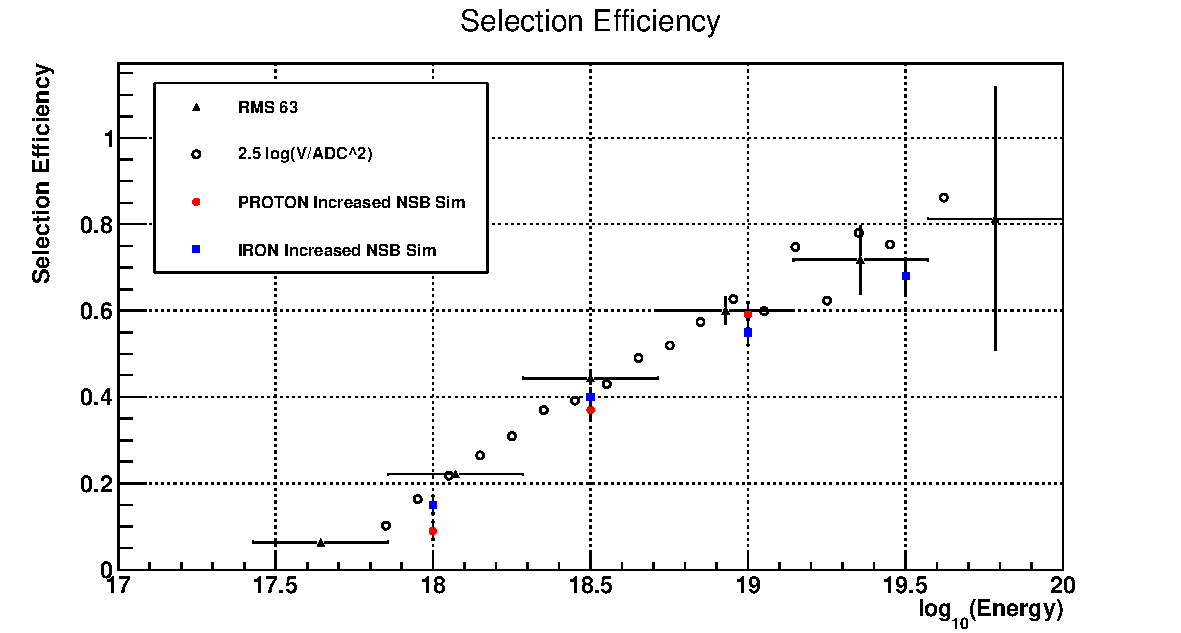
\includegraphics[width=\textwidth]{chapters/graphs/SelectionEff/SelectionEff_errorbars_10timesNSB.pdf}
\caption{Selection Efficiency plot containing data from both the Smearing method and simulated showers. These results are compared to the work done by M. Unger.}
\end{figure}

\section{Resolution and Bias}

To further evaluate the effects of increasing the NSB on the quality of the reconstructed EAS data, I look at the resolution and bias of both the reconstructed energy and reconstructed Xmax. A quick reminder that Xmax is the measurement of the brightest part of the shower relating to the maximum number of particles produced. For the smearing method the energy and Xmax bias is comparing to the measured data taken at standard NSB levels to the reconstructed with the increased NSB levels. For the simulations the energy and Xmax bias can be calculated using the true energy and Xmax values used to generate each EAS profile.

The trend of the energy resolution for both methods is that as the energy of the EAS event increases the bias decreases. This was expected as the energy of the shower increases the brighter and longer the track that is observed. A brighter and longer track allows for a better reconstruction.

- Need to find out what's a good bias value for energy and Xmax.

the energy and Xamx bias is calcualted via:
\begin{eqnarray}
\Delta \mathrm{E} &=& \frac{\mathrm{E}_{\mathrm{recon}} - \mathrm{E}_{\mathrm{true}}}{\mathrm{E}_{\mathrm{true}}}  \label{eq:energybias_sim} \\
\Delta \mathrm{E} &=& \frac{\mathrm{E}_{\mathrm{IncreasedNSB}} - \mathrm{E}_{\mathrm{StandardNSB}}}{\mathrm{E}_{\mathrm{StandardNSB}}} \label{eq:energybias_data} \\
\Delta \mathrm{Xmax} &=& \mathrm{Xmax}_{\mathrm{recon}} - \mathrm{Xmax}_{\mathrm{true}} \label{eq:xmaxbias_sim} \\
\Delta \mathrm{Xmax} &=& \mathrm{Xmax}_{\mathrm{IncreasedNSB}} - \mathrm{Xmax}_{\mathrm{StandardNSB}}\label{eq:xmaxbias_data}
\end{eqnarray}
Eq. \ref{eq:energybias_sim} and Eq. \ref{eq:xmaxbias_sim} are used on the simulated data sets while Eq. \ref{eq:energybias_data} and Eq. \ref{eq:xmaxbias_data} is used on the smeared data set.

The energy and Xmax resolution is calculated via:
\begin{eqnarray}
\sigma_{\mathrm{res}} &=& \left( \frac{1}{\mathrm{N}} \sum \frac{1}{\sigma^2_i} \right)^{1/2}
\end{eqnarray}


\begin{figure}
\centering
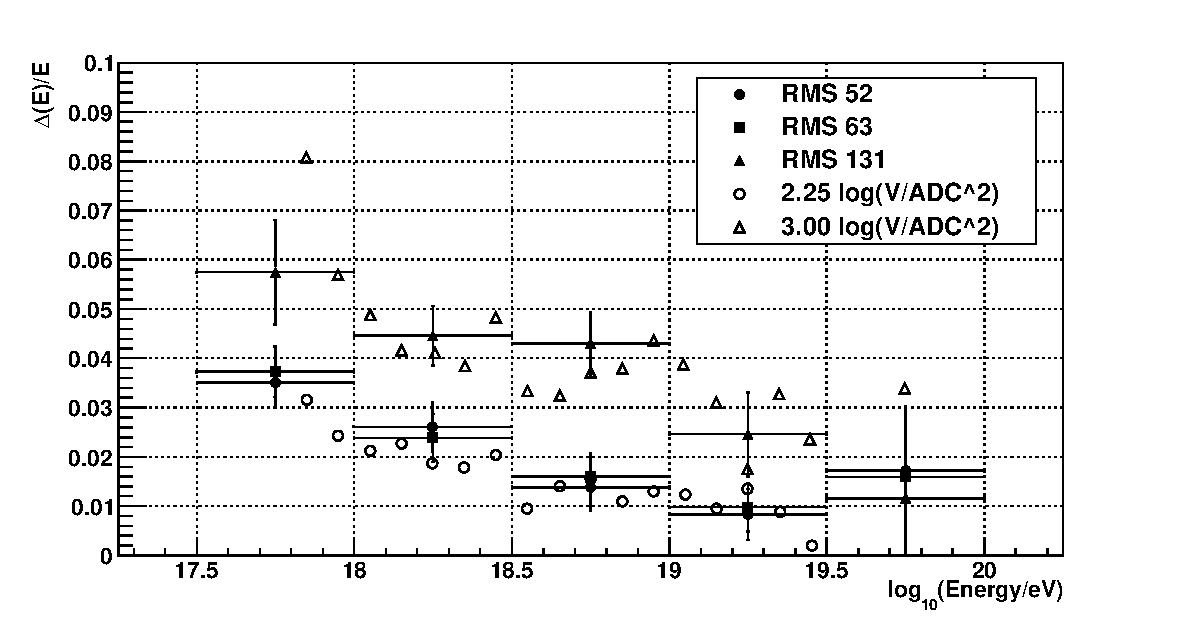
\includegraphics[width=\textwidth]{chapters/graphs/SelectionEff/Smearing_RealData_EnergyBias.pdf}
\caption{Energy Bias using Smearing Method.}
\vspace{3mm}
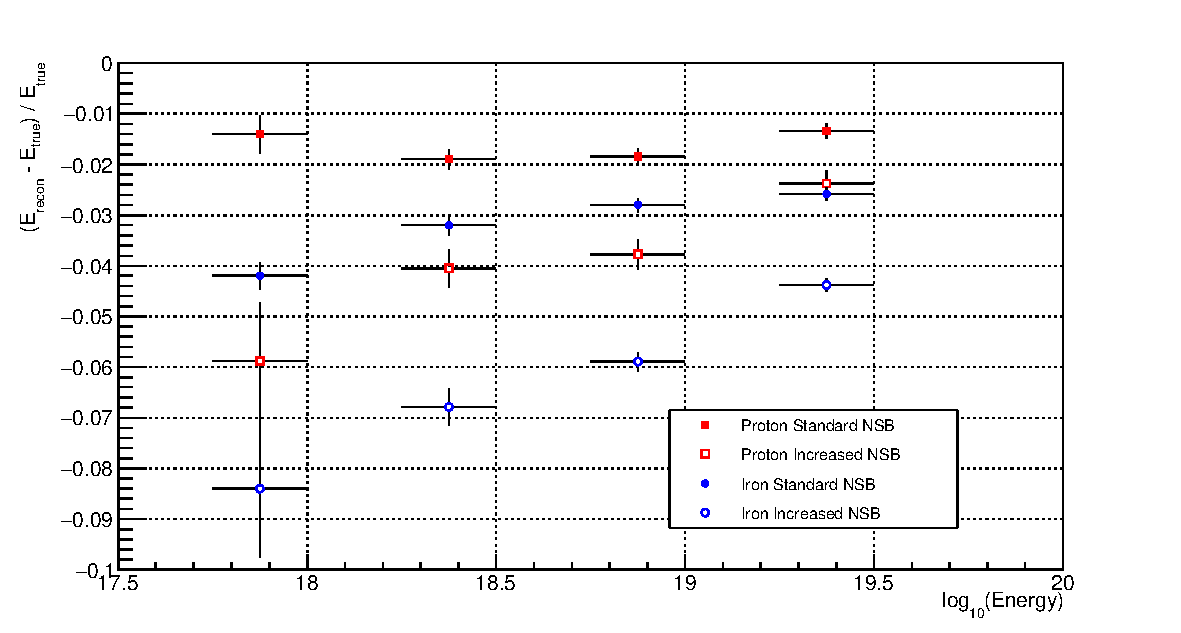
\includegraphics[width=\textwidth]{chapters/graphs/SelectionEff/Simulation_ProtonIron_EnergyBias.pdf}
\caption{Energy Bias using simulated data.}
\end{figure}

\begin{figure}
\centering
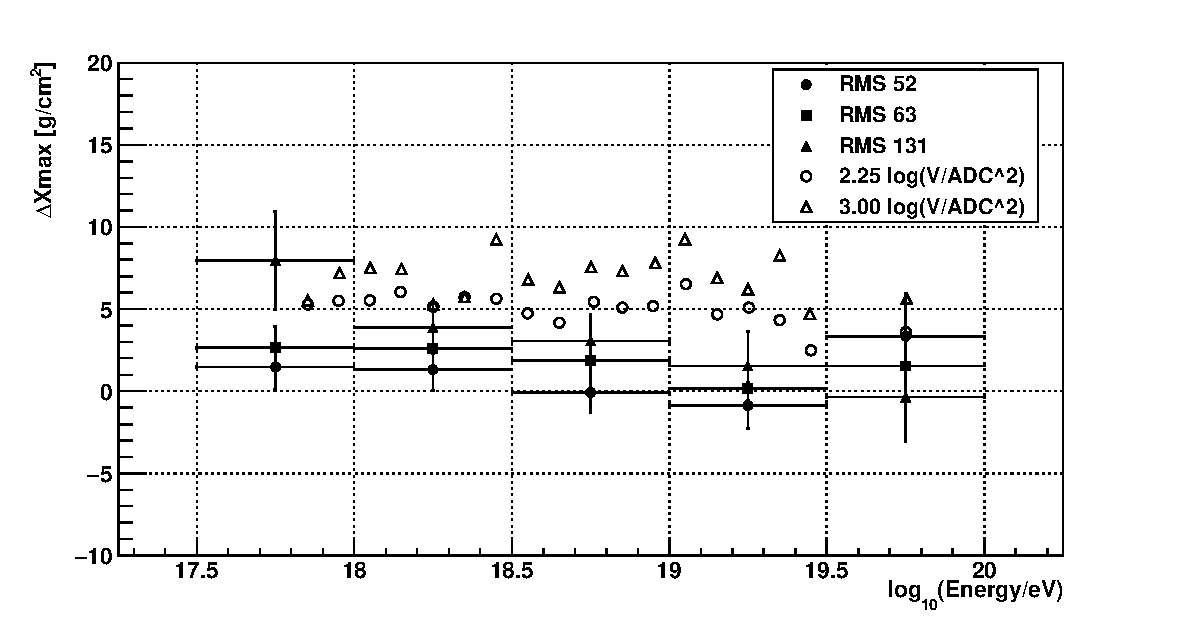
\includegraphics[width=\textwidth]{chapters/graphs/SelectionEff/Smearing_RealData_XmaxBias.pdf}
\caption{Xmax Bias using Smearing Method.}
\vspace{3mm}
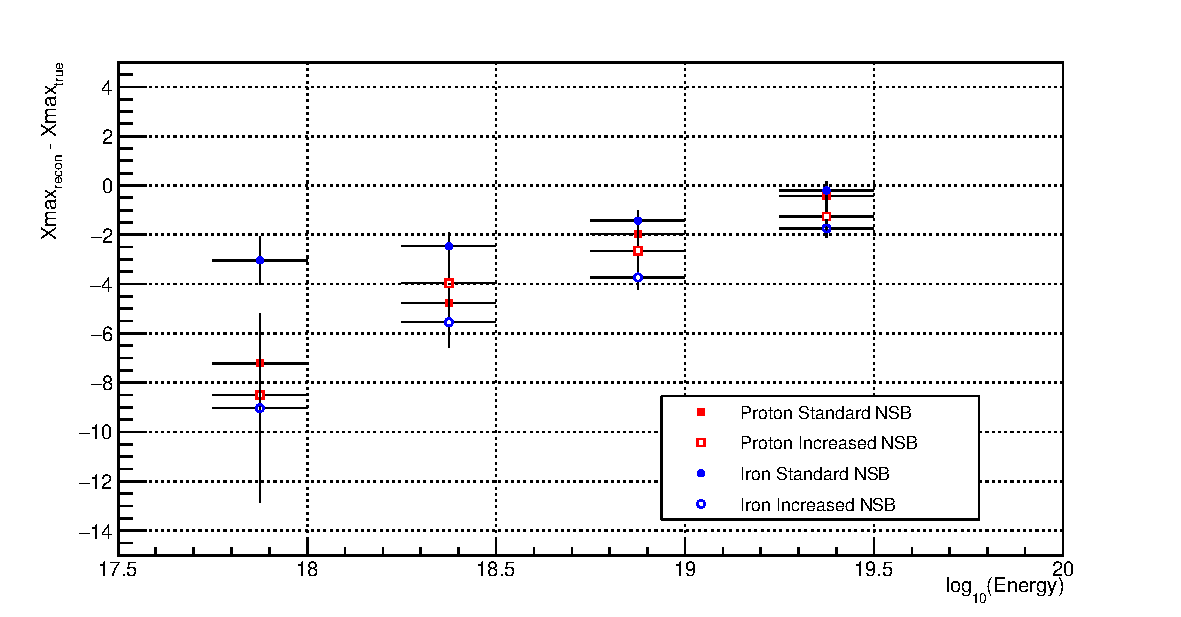
\includegraphics[width=\textwidth]{chapters/graphs/SelectionEff/Simulation_ProtonIron_XmaxBias.pdf}
\caption{Xmax Bias using simulated data.}
\end{figure}

\begin{figure}
\centering
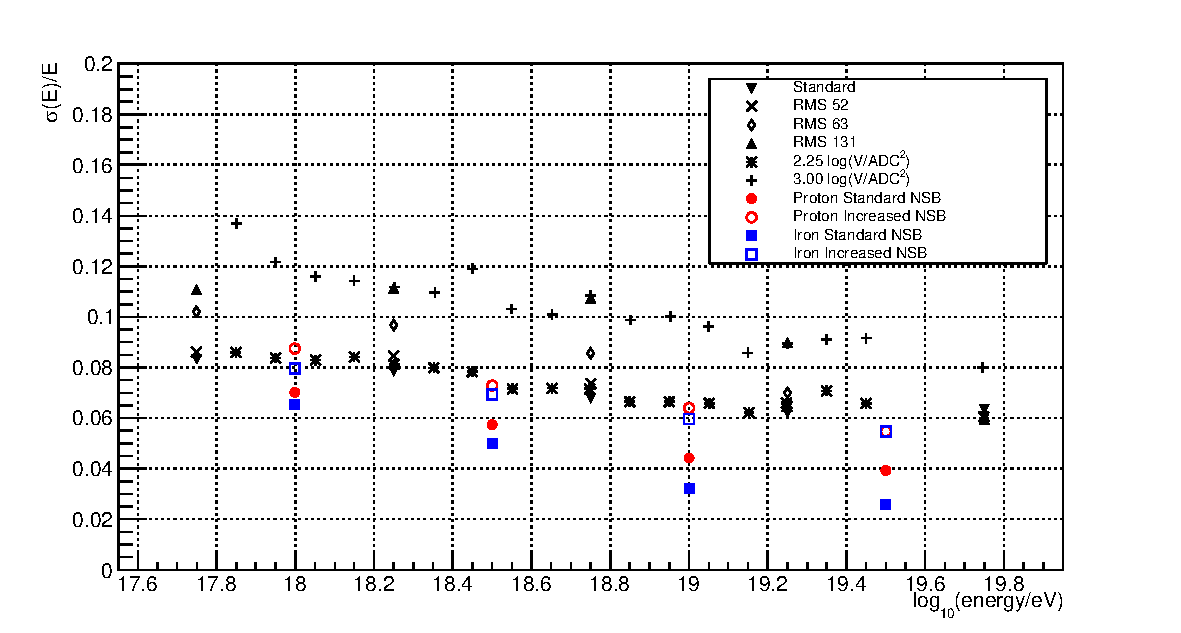
\includegraphics[width=\textwidth]{chapters/graphs/SelectionEff/Combined_EnergyRes_All.pdf}
\caption{Energy Resolution using both Smearing Method data and simulated showers.}
\vspace{3mm}
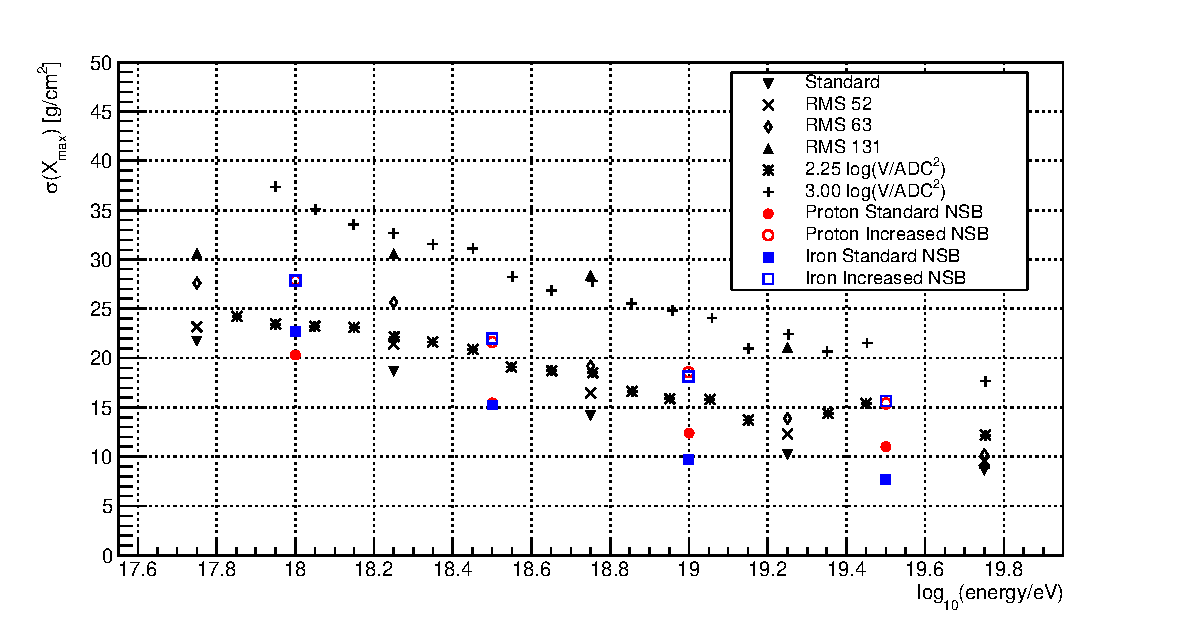
\includegraphics[width=\textwidth]{chapters/graphs/SelectionEff/Combined_XmaxRes_All.pdf}
\caption{Xmax Resolution using both Smearing Method data and simulated showers.}
\end{figure}

\subsection{Comparing Simulated Data to Real Data}

\textbf{Think about where to locate this section.}

Comparing the simulated data with real data. Checking to make sure that the simulation data is a good representation of reality. Looking at the Xmax distribution there is no need for a direction comparison as I only simulated proton and iron primaries and was not concern with have a particular mixtures. The other parameter I checked was the zenith angle distribution, distance to Xmax and distance to the shower axis (R$_{\mathrm{P}}$). The simulated profiles have similar shapes when both histograms are normalised to area of 1. For zenith angle distribution I simulated the EAS events upto a zenith angle of 60\textdegree so that the reason for the cut-off in the simulated data.

\begin{figure}
\centering
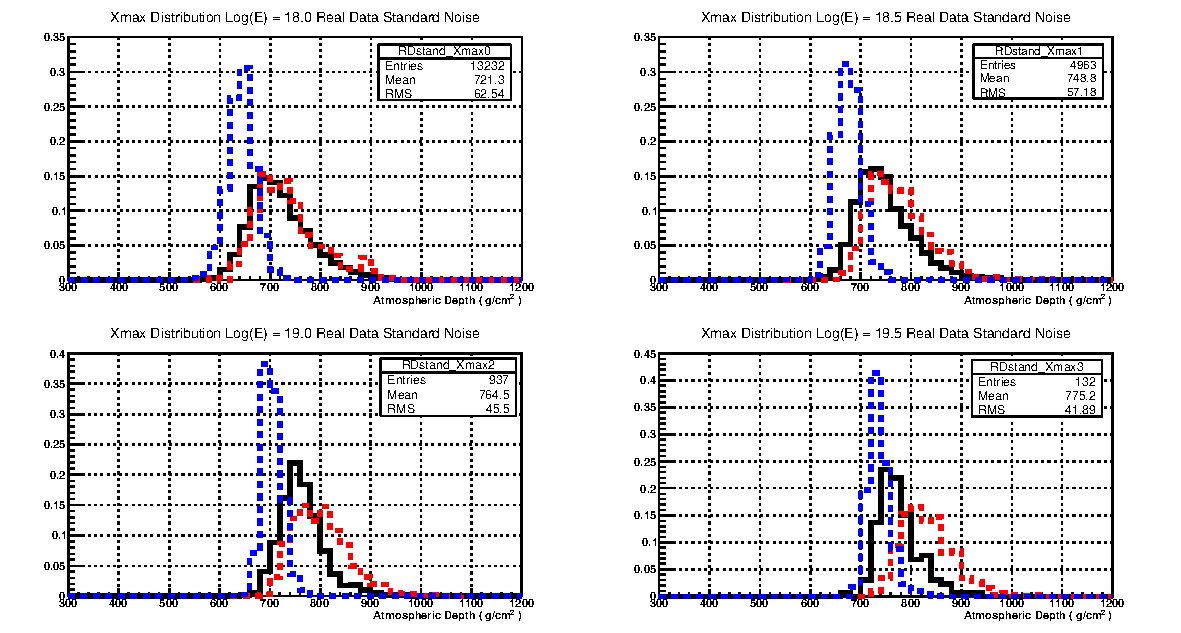
\includegraphics[width=\textwidth]{chapters/graphs/SelectionEff/RealDataAndSim_XmaxDistComp.pdf}
\caption{Distribution of Xmax with Real Data and simulation of proton and iron showers.}
\vspace{3mm}
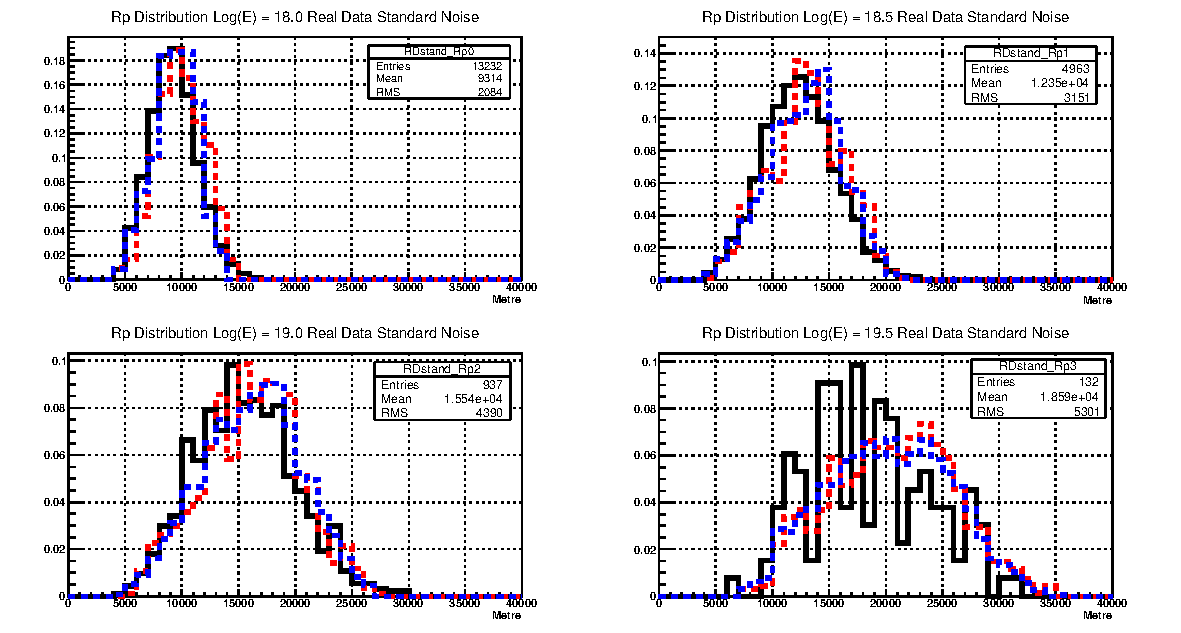
\includegraphics[width=\textwidth]{chapters/graphs/SelectionEff/RealDataAndSim_RpDistComp.pdf}
\caption{Distribution of Rp with Real Data and simulation of proton and iron showers.}
\end{figure}

\begin{figure}
\centering
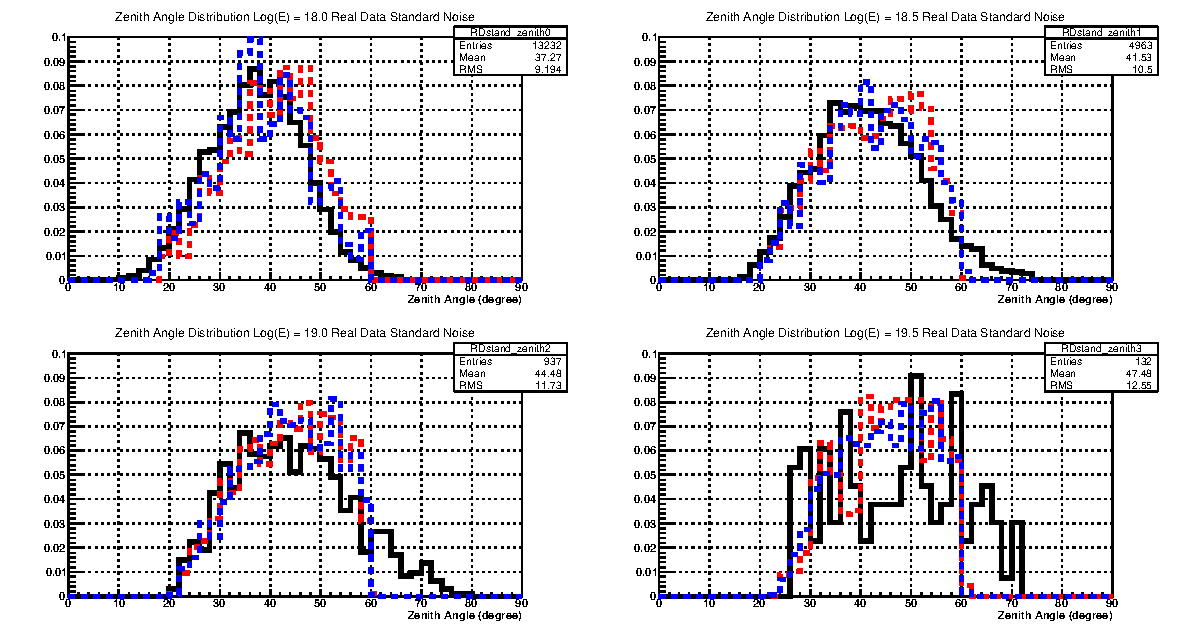
\includegraphics[width=\textwidth]{chapters/graphs/SelectionEff/RealDataAndSim_ZenithDistComp.pdf}
\caption{Distribution of Zenith angle with Real Data and simulation of proton and iron showers.}
\vspace{3mm}
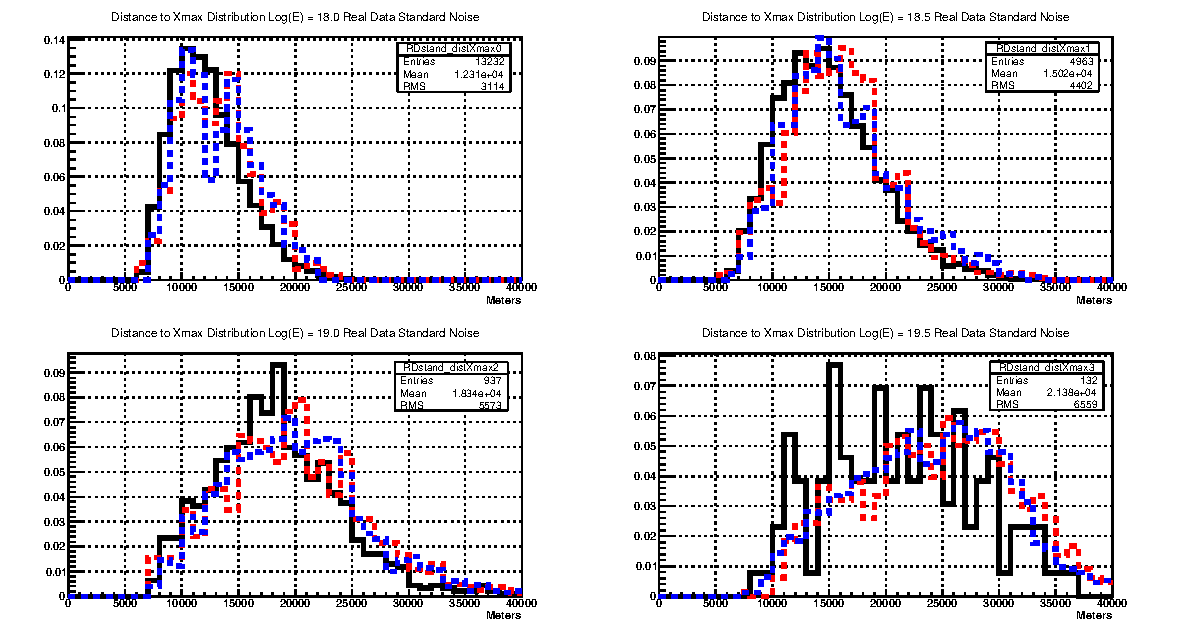
\includegraphics[width=\textwidth]{chapters/graphs/SelectionEff/RealDataAndSim_DistToXmaxDistComp.pdf}
\caption{Distribution of Distance to Xmax with Real Data and simulation of proton and iron showers.}
\end{figure}

\section{EAS Track Length in the FD's}

One other parameter that was investigate was the shower track length observed by the FD's. It was expected that as the NSB increased the average observed shower track length would decrease. For both the smearing and simulation this trend was observed by not in a significant way. This is shown in Fig. \ref{fig:TrackLength_Smearing} and Fig. \ref{fig:TrackLength_Sim}.  There was a thought about trying to extended track length into the noisy pixels as it would be known that would be photons observed at the start and end of the track. The measured data shows that this is not needed as not much of the track is lost with increased NSB. Especially at the highest energy bins where the most interest lays. 

\begin{figure}
\centering
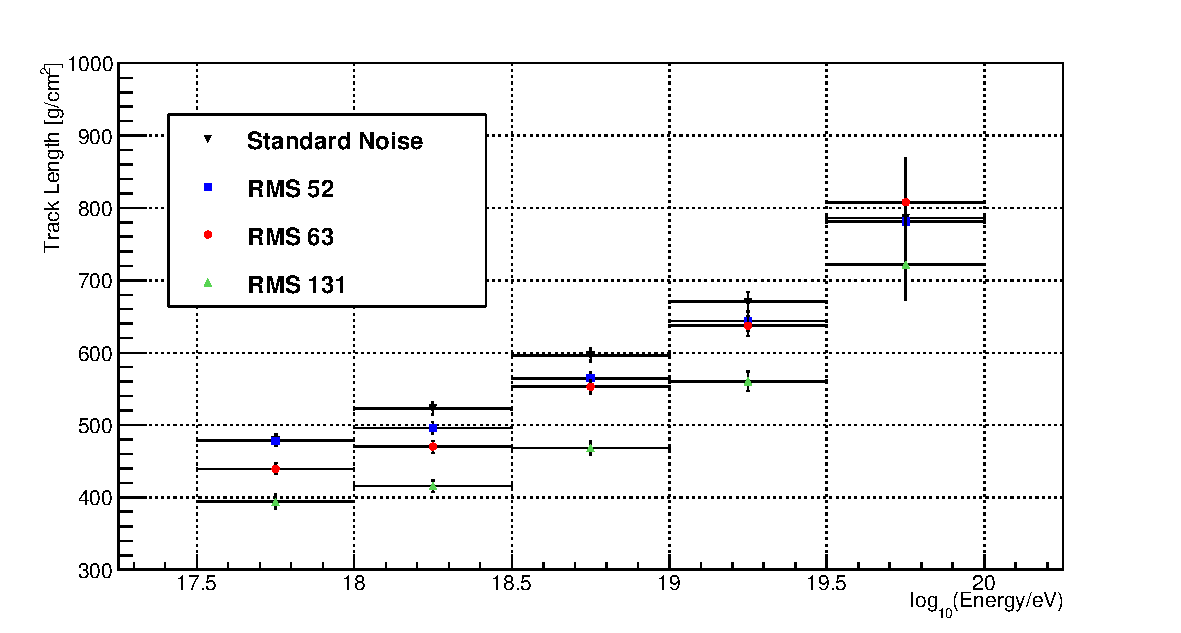
\includegraphics[width=\textwidth]{chapters/graphs/SelectionEff/Smearing_TrackLength_DiffNSBlevels.pdf}
\caption{Track length using Smearing method.} \label{fig:TrackLength_Smearing}
\vspace{3mm}
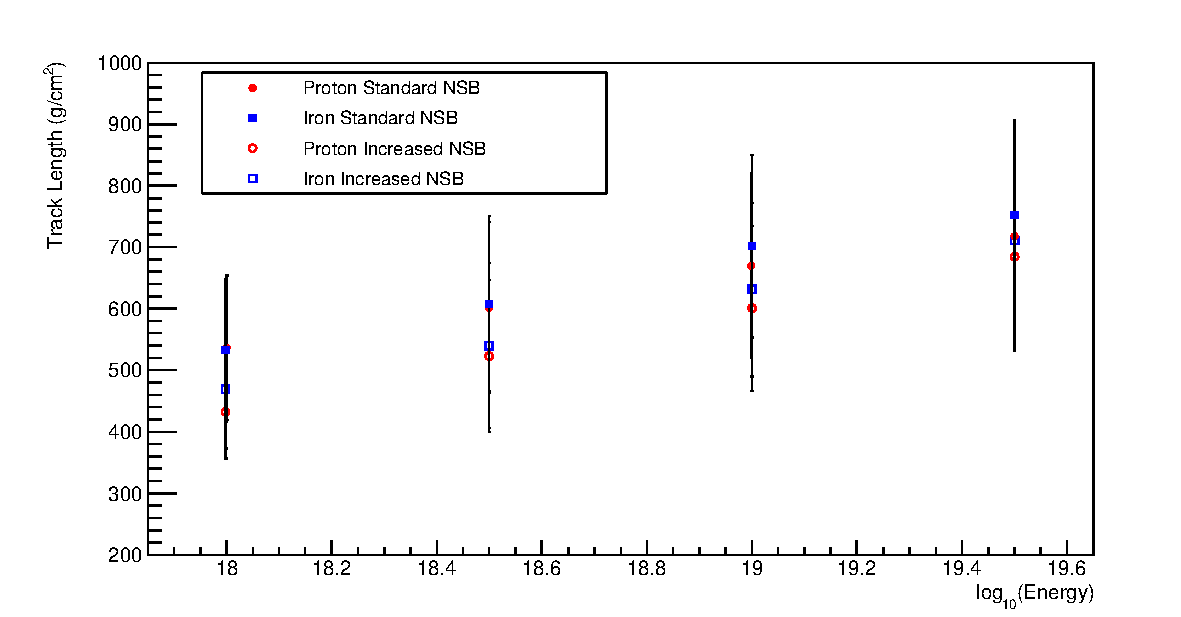
\includegraphics[width=\textwidth]{chapters/graphs/SelectionEff/Simulation_TrackLength_Comb_StandANdIncreasedNSB.pdf}
\caption{Track length using simulation of proton and iron CONEX showers.} \label{fig:TrackLength_Sim}
\end{figure}

\chapter{Quantifying Characteristics of the FD PMT}\label{Ch:PMTCharacter}

Characterising the PMT at 600V and 900V
\begin{itemize}
\item Using the characteristics of the PMT at 900V as a baseline
\item Measure linearity
\item ND filters bs Two LED method
\item Pulse shape?
\item temperature effects
\item dark noise?
\end{itemize}
\chapter[Computer Simulation of FD PMT]{\centering Computer Simulation of FD PMT \\}\label{Ch:CompSimPMT}

Simulating the FD PMT under differing NSB and for different reasons.
\begin{itemize}
\item Theoretical value for Gain Variance
\item PMT Gain Variance
\item Show both for flat distribution and Gaussian variations for dynodes
\item Results
\item FD FLT under increased NSB
\item Kv simulation under increased NSB?
\end{itemize}

\begin{figure}
\centering
\begin{subfigure}[b]{0.44\textwidth}
\adjincludegraphics[width=\textwidth, trim={0 0 0 {0.08\height}}, clip]{chapters/graphs/PMTsimulation/ElectronsLeaving_PoissonFit_Dynode1_5e4.pdf}
\caption{Distribution of simulated electrons leaving dynode 1. The red line is a fitted Poisson distribution.}
\end{subfigure}
\hspace{3mm}
\begin{subfigure}[b]{0.44\textwidth}
\adjincludegraphics[width=\textwidth, trim={0 0 0 {0.08\height}}, clip]{chapters/graphs/PMTsimulation/ElectronsLeaving_Dynode2_5e4.pdf}
\caption{Distribution of simulated electrons leaving dynode 2. The red line is a fitted Gaussian distribution.}
\end{subfigure}

\vspace{3mm}

\begin{subfigure}[b]{0.44\textwidth}
\adjincludegraphics[width=\textwidth, trim={0 0 0 {0.08\height}}, clip]{chapters/graphs/PMTsimulation/ElectronsLeaving_Dynode3_5e4.pdf}
\caption{Distribution of simulated electrons leaving dynode 3. The red line is a fitted Poisson distribution.}
\end{subfigure}
\hspace{3mm}
\begin{subfigure}[b]{0.44\textwidth}
\adjincludegraphics[width=\textwidth, trim={0 0 0 {0.08\height}}, clip]{chapters/graphs/PMTsimulation/ElectronsLeaving_Dynode4_5e4.pdf}
\caption{Distribution of simulated electrons leaving dynode 4. The red line is a fitted Gaussian distribution.}
\end{subfigure}

\vspace{3mm}

\begin{subfigure}[b]{0.44\textwidth}
\adjincludegraphics[width=\textwidth, trim={0 0 0 {0.08\height}}, clip]{chapters/graphs/PMTsimulation/ElectronsLeaving_Dynode5_5e4.pdf}
\caption{Distribution of simulated electrons leaving dynode 5. The red line is a fitted Poisson distribution.}
\end{subfigure}
\hspace{3mm}
\begin{subfigure}[b]{0.44\textwidth}
\adjincludegraphics[width=\textwidth, trim={0 0 0 {0.08\height}}, clip]{chapters/graphs/PMTsimulation/ElectronsLeaving_Dynode6_5e4.pdf}
\caption{Distribution of simulated electrons leaving dynode 6. The red line is a fitted Gaussian distribution.}
\end{subfigure}

\vspace{3mm}

\begin{subfigure}[b]{0.44\textwidth}
\adjincludegraphics[width=\textwidth, trim={0 0 0 {0.08\height}}, clip]{chapters/graphs/PMTsimulation/ElectronsLeaving_Dynode7_5e4.pdf}
\caption{Distribution of simulated electrons leaving dynode 7. The red line is a fitted Poisson distribution.}
\end{subfigure}
\hspace{3mm}
\begin{subfigure}[b]{0.44\textwidth}
\adjincludegraphics[width=\textwidth, trim={0 0 0 {0.08\height}}, clip]{chapters/graphs/PMTsimulation/ElectronsLeaving_Dynode8_5e4.pdf}
\caption{Distribution of simulated electrons leaving dynode 8. The red line is a fitted Gaussian distribution.}
\end{subfigure}
\end{figure}

\begin{figure}
\centering
\begin{subfigure}[b]{0.44\textwidth}
\adjincludegraphics[width=\textwidth, trim={0 0 0 {0.08\height}}, clip]{chapters/graphs/PMTsimulation/PMTsim_1PE_TypeC_DynodeSigm0_5e5.pdf}
\caption{Simulated observed signal from PMT anode with 8 stages and gain of 5 $\times \ 10^5$. Poisson fluctuations at each stage only. No each Gaussian broadening at any dynode.}
\end{subfigure}
\hspace{3mm}
\begin{subfigure}[b]{0.44\textwidth}
\adjincludegraphics[width=\textwidth, trim={0 0 0 {0.08\height}}, clip]{chapters/graphs/PMTsimulation/PMTsim_1PE_TypeC_DynodeSigm0_1_5e5.pdf}
\caption{Simulated observed signal from PMT anode with 8 stages and gain of 5 $\times \ 10^5$. Poisson fluctuations at each stage only. Added Gaussian braodening at each dynode of 10\%.}
\end{subfigure}

\vspace{3mm}

\begin{subfigure}[b]{0.44\textwidth}
\adjincludegraphics[width=\textwidth, trim={0 0 0 {0.08\height}}, clip]{chapters/graphs/PMTsimulation/PMTsim_1PE_TypeC_DynodeSigm0_2_5e5.pdf}
\caption{Simulated observed signal from PMT anode with 8 stages and gain of 5 $\times \ 10^5$. Poisson fluctuations at each stage only. Added Gaussian braodening at each dynode of 20\%.}
\end{subfigure}
\hspace{3mm}
\begin{subfigure}[b]{0.44\textwidth}
\adjincludegraphics[width=\textwidth, trim={0 0 0 {0.08\height}}, clip]{chapters/graphs/PMTsimulation/PMTsim_1PE_TypeC_DynodeSigm0_3_5e5.pdf}
\caption{Simulated observed signal from PMT anode with 8 stages and gain of 5 $\times \ 10^5$. Poisson fluctuations at each stage only. Added Gaussian braodening at each dynode of 30\%.}
\end{subfigure}

\vspace{3mm}

\begin{subfigure}[b]{0.44\textwidth}
\adjincludegraphics[width=\textwidth, trim={0 0 0 {0.08\height}}, clip]{chapters/graphs/PMTsimulation/PMTsim_1PE_TypeC_DynodeSigm0_4_5e5.pdf}
\caption{Simulated observed signal from PMT anode with 8 stages and gain of 5 $\times \ 10^5$. Poisson fluctuations at each stage only. Added Gaussian braodening at each dynode of 40\%.}
\end{subfigure}
\hspace{3mm}
\begin{subfigure}[b]{0.44\textwidth}
\adjincludegraphics[width=\textwidth, trim={0 0 0 {0.08\height}}, clip]{chapters/graphs/PMTsimulation/PMTsim_1PE_TypeC_DynodeSigm0_5_5e5.pdf}
\caption{Simulated observed signal from PMT anode with 8 stages and gain of 5 $\times \ 10^5$. Poisson fluctuations at each stage only. Added Gaussian braodening at each dynode of 50\%.}
\end{subfigure}
\end{figure}

\begin{figure}
\centering
\begin{subfigure}[b]{0.44\textwidth}
\adjincludegraphics[width=\textwidth, trim={0 0 0 {0.08\height}}, clip]{chapters/graphs/PMTsimulation/PMTsim_1PE_TypeC_DynodeSigm0_5e4.pdf}
\caption{Simulated observed signal from PMT anode with 8 stages and gain of 5 $\times \ 10^4$. Poisson fluctuations at each stage only. No each Gaussian broadening at any dynode.}
\end{subfigure}
\hspace{3mm}
\begin{subfigure}[b]{0.44\textwidth}
\adjincludegraphics[width=\textwidth, trim={0 0 0 {0.08\height}}, clip]{chapters/graphs/PMTsimulation/PMTsim_1PE_TypeC_DynodeSigm0_1_5e4.pdf}
\caption{Simulated observed signal from PMT anode with 8 stages and gain of 5 $\times \ 10^4$. Poisson fluctuations at each stage only. Added Gaussian braodening at each dynode of 10\%.}
\end{subfigure}

\vspace{3mm}

\begin{subfigure}[b]{0.44\textwidth}
\adjincludegraphics[width=\textwidth, trim={0 0 0 {0.08\height}}, clip]{chapters/graphs/PMTsimulation/PMTsim_1PE_TypeC_DynodeSigm0_2_5e4.pdf}
\caption{Simulated observed signal from PMT anode with 8 stages and gain of 5 $\times \ 10^4$. Poisson fluctuations at each stage only. Added Gaussian braodening at each dynode of 20\%.}
\end{subfigure}
\hspace{3mm}
\begin{subfigure}[b]{0.44\textwidth}
\adjincludegraphics[width=\textwidth, trim={0 0 0 {0.08\height}}, clip]{chapters/graphs/PMTsimulation/PMTsim_1PE_TypeC_DynodeSigm0_3_5e4.pdf}
\caption{Simulated observed signal from PMT anode with 8 stages and gain of 5 $\times \ 10^4$. Poisson fluctuations at each stage only. Added Gaussian braodening at each dynode of 30\%.}
\end{subfigure}

\vspace{3mm}

\begin{subfigure}[b]{0.44\textwidth}
\adjincludegraphics[width=\textwidth, trim={0 0 0 {0.08\height}}, clip]{chapters/graphs/PMTsimulation/PMTsim_1PE_TypeC_DynodeSigm0_4_5e4.pdf}
\caption{Simulated observed signal from PMT anode with 8 stages and gain of 5 $\times \ 10^4$. Poisson fluctuations at each stage only. Added Gaussian braodening at each dynode of 40\%.}
\end{subfigure}
\hspace{3mm}
\begin{subfigure}[b]{0.44\textwidth}
\adjincludegraphics[width=\textwidth, trim={0 0 0 {0.08\height}}, clip]{chapters/graphs/PMTsimulation/PMTsim_1PE_TypeC_DynodeSigm0_5_5e4.pdf}
\caption{Simulated observed signal from PMT anode with 8 stages and gain of 5 $\times \ 10^4$. Poisson fluctuations at each stage only. Added Gaussian braodening at each dynode of 50\%.}
\end{subfigure}
\end{figure}

\begin{figure}
\centering
\begin{subfigure}[b]{0.44\textwidth}
\adjincludegraphics[width=\textwidth, trim={0 0 0 {0.08\height}}, clip]{chapters/graphs/PMTsimulation/PMTsim_1PE_TypeC_DynodeSigm0_5e3.pdf}
\caption{Simulated observed signal from PMT anode with 8 stages and gain of 5 $\times \ 10^3$. Poisson fluctuations at each stage only. No each Gaussian broadening at any dynode.}
\end{subfigure}
\hspace{3mm}
\begin{subfigure}[b]{0.44\textwidth}
\adjincludegraphics[width=\textwidth, trim={0 0 0 {0.08\height}}, clip]{chapters/graphs/PMTsimulation/PMTsim_1PE_TypeC_DynodeSigm0_1_5e3.pdf}
\caption{Simulated observed signal from PMT anode with 8 stages and gain of 5 $\times \ 10^3$. Poisson fluctuations at each stage only. Added Gaussian braodening at each dynode of 10\%.}
\end{subfigure}

\vspace{3mm}

\begin{subfigure}[b]{0.44\textwidth}
\adjincludegraphics[width=\textwidth, trim={0 0 0 {0.08\height}}, clip]{chapters/graphs/PMTsimulation/PMTsim_1PE_TypeC_DynodeSigm0_2_5e3.pdf}
\caption{Simulated observed signal from PMT anode with 8 stages and gain of 5 $\times \ 10^3$. Poisson fluctuations at each stage only. Added Gaussian braodening at each dynode of 20\%.}
\end{subfigure}
\hspace{3mm}
\begin{subfigure}[b]{0.44\textwidth}
\adjincludegraphics[width=\textwidth, trim={0 0 0 {0.08\height}}, clip]{chapters/graphs/PMTsimulation/PMTsim_1PE_TypeC_DynodeSigm0_3_5e3.pdf}
\caption{Simulated observed signal from PMT anode with 8 stages and gain of 5 $\times \ 10^3$. Poisson fluctuations at each stage only. Added Gaussian braodening at each dynode of 30\%.}
\end{subfigure}

\vspace{3mm}

\begin{subfigure}[b]{0.44\textwidth}
\adjincludegraphics[width=\textwidth, trim={0 0 0 {0.08\height}}, clip]{chapters/graphs/PMTsimulation/PMTsim_1PE_TypeC_DynodeSigm0_4_5e3.pdf}
\caption{Simulated observed signal from PMT anode with 8 stages and gain of 5 $\times \ 10^3$. Poisson fluctuations at each stage only. Added Gaussian braodening at each dynode of 40\%.}
\end{subfigure}
\hspace{3mm}
\begin{subfigure}[b]{0.44\textwidth}
\adjincludegraphics[width=\textwidth, trim={0 0 0 {0.08\height}}, clip]{chapters/graphs/PMTsimulation/PMTsim_1PE_TypeC_DynodeSigm0_5_5e3.pdf}
\caption{Simulated observed signal from PMT anode with 8 stages and gain of 5 $\times \ 10^3$. Poisson fluctuations at each stage only. Added Gaussian braodening at each dynode of 50\%.}
\end{subfigure}
\end{figure}

\begin{figure}
\centering
\begin{subfigure}[b]{0.44\textwidth}
\adjincludegraphics[width=\textwidth, trim={0 0 0 {0.08\height}}, clip]{chapters/graphs/PMTsimulation/FLT_simulation_2_71pePER100ns.pdf}
\caption{FLT simulation with NSB of 2.71 pe / 100ns.}
\end{subfigure}
\hspace{3mm}
\begin{subfigure}[b]{0.44\textwidth}
\adjincludegraphics[width=\textwidth, trim={0 0 0 {0.08\height}}, clip]{chapters/graphs/PMTsimulation/FLT_simulation_6_60pePER100ns.pdf}
\caption{FLT simulation with NSB of 6.60 pe / 100ns.}
\end{subfigure}

\vspace{3mm}

\begin{subfigure}[b]{0.44\textwidth}
\adjincludegraphics[width=\textwidth, trim={0 0 0 {0.08\height}}, clip]{chapters/graphs/PMTsimulation/FLT_simulation_46_8pePER100ns.pdf}
\caption{FLT simulation with NSB of 46.8 pe / 100ns.}
\end{subfigure}
\hspace{3mm}
\begin{subfigure}[b]{0.44\textwidth}
\adjincludegraphics[width=\textwidth, trim={0 0 0 {0.08\height}}, clip]{chapters/graphs/PMTsimulation/FLT_simulation_65_8pePER100ns.pdf}
\caption{FLT simulation with NSB of 65.8 pe / 100ns.}
\end{subfigure}

\vspace{3mm}
\begin{subfigure}[b]{0.44\textwidth}
\adjincludegraphics[width=\textwidth, trim={0 0 0 {0.08\height}}, clip]{chapters/graphs/PMTsimulation/FLT_simulation_263pePER100ns.pdf}
\caption{FLT simulation with NSB of 263 pe / 100ns.}
\end{subfigure}
\hspace{3mm}
\begin{subfigure}[b]{0.44\textwidth}
\adjincludegraphics[width=\textwidth, trim={0 0 0 {0.08\height}}, clip]{chapters/graphs/PMTsimulation/FLT_simulation_657pePER100ns.pdf}
\caption{FLT simulation with NSB of 657 pe / 100ns.}
\end{subfigure}
\end{figure}
\chapter[Measuring FD PMT Gain Variance with CalA Data]{\centering Measuring FD PMT Gain Variance with CalA Data \\}\label{Ch:GainVariance}

Measuring Gain Variance of FD PMT with CalA Data
\begin{itemize}
\item Measuring Gain Variance in the lab did not work. Equipment was not sensitive enough to the low current.
\item There was issues with calibrating the LED light source with another PMT (QE curve and wavelength response not the same?)
\item Using Low/Standard measurements of CalA to find Gain Variance Ratio
\item Two different methods
\item Bootstrap method to find uncertainties on Method 2
\end{itemize}

\section{Using CalA to measure relative changes in Gain Variance}

Using CalA data from the FD telescopes to measure the relative changes in PMT  gain variance as the gain is changed by a factor of 10. CalA data is calibration data used to monitor any changes in PMT gain as a function of time. CalA is performed at the beginning and end of a nightly observation done with the FDs. Pulses from a monitored light source are piped to point at the camera. There are 50 pulses sent with a width of approximately 60 $\mu$s.

\textbf{show image of CalA pulse}

One of the values that can be calculated from the CalA is a value denoted K$_{\mathrm{V}}$. K$_{\mathrm{V}}$ is calculated via:
\begin{equation}
\mathrm{K}_{\mathrm{V}} = \frac{\mathrm{Mean}}{\mathrm{Sigma}^2} = \frac{10}{2 \times \mathrm{G} (1 + \mathrm{V}_{\mathrm{G}}) \times \mathrm{F}}
\end{equation}
Mean is the average ADC count of the observed CalA pulse seen the FD pixel, sigma$^2$ is the variance calculated around fit to the signal in ADC$^2$. The signal has a slope due to the effects of a capacitor used to remove the DC component of the signal. The slope is proportional to the time constant of the capacitor employed. G is the PMT gain, F is the noise equivalent bandwidth (Hz) and V$_{\mathrm{G}}$ is the PMT gain variance.

The absolute value of the gain variance cannot be found but using K$_{\mathrm{V}}$ a relative change can be found. This is useful for the collaboration simulations as a Gain variance is coded for the PMT at standard voltage settings. Finding out the relative change in gain variance would be useful to be used for simulations of the FD PMTs at a lower voltage settings (IE. 600V).

The method used to measure the ratio in gain variance is to take the calculated means and sigmas from the pulses and then find a ratio between the K$_{\mathrm{V}}$ and Gains at the two different voltage settings.
\begin{eqnarray}
\mathrm{K} = \frac{\mathrm{Mean}}{\mathrm{Sigma}^2} &=& \frac{10}{2 \times \mathrm{G} (1 + \mathrm{V}_{\mathrm{G}}) \times \mathrm{F}} \\ 
\frac{\left(\mathrm{K}_{\mathrm{V}}\right)_{\mathrm{Low}}}{\left(\mathrm{K}_{\mathrm{V}}\right)_{\mathrm{Stand}}} &=& \frac{\mathrm{Mean}_{\mathrm{Low}}}{\mathrm{Sigma}^2_{\mathrm{Low}}} \div \frac{\mathrm{Mean}_{\mathrm{Stand}}}{\mathrm{Sigma}^2_{\mathrm{Stand}}} \\ 
\frac{\mathrm{Mean}_{\mathrm{Low}}}{\mathrm{Sigma}^2_{\mathrm{Low}}} \div \frac{\mathrm{Mean}_{\mathrm{Stand}}}{\mathrm{Sigma}^2_{\mathrm{Stand}}} &=& \frac{\mathrm{G}_{\mathrm{Stand}} (1 + \mathrm{V}_{\mathrm{G}})_{\mathrm{Stand}}}{\mathrm{G}_{\mathrm{Low}} (1 + \mathrm{V}_{\mathrm{G}})_{\mathrm{Low}}} \\
\frac{\mathrm{G}_{\mathrm{Stand}}}{\mathrm{G}_{\mathrm{Low}}} &=& \frac{\mathrm{Mean}_{\mathrm{Stand}}}{\mathrm{Mean}_{\mathrm{Low}}} \\
\frac{(1 + \mathrm{V}_{\mathrm{G}})_{\mathrm{Low}}}{(1 + \mathrm{V}_{\mathrm{G}})_{\mathrm{Stand}}} &=& \frac{\mathrm{Sigma}^2_{\mathrm{Low}} \times \mathrm{Mean}^2_{\mathrm{Stand}}}{\mathrm{Sigma}^2_{\mathrm{Stand}} \times \mathrm{Mean}^2_{\mathrm{Low}}}
\end{eqnarray}

\section{Electronic Noise}

Investigated the consistency of the electronic noise across a set of 50 CalA traces. The consistency was looked as there is only about 140 bins of noise before the signal pulse start. Therefore finding an accurate mean and variance of the electronic noise on an individual pulse is difficult. An accurate measurement of the electronic noise mean and variance was required as the measured gain variance ratio was only a few percent.

\textbf{Need to show electronic noise as function of time.}

An example of a pixel electronic noise trace is shown in Fig. \ref{}. It can be seen in this figure that stitching all of the noise bins from the 50 traces is remarkably stable. This result allows for all the noise for a single PMT pixel to be place into a histogram to find a more accurate value for the mean and variance.

\begin{figure} % Electronic Noise Distribution
\centering
\begin{subfigure}[b]{0.95\textwidth}
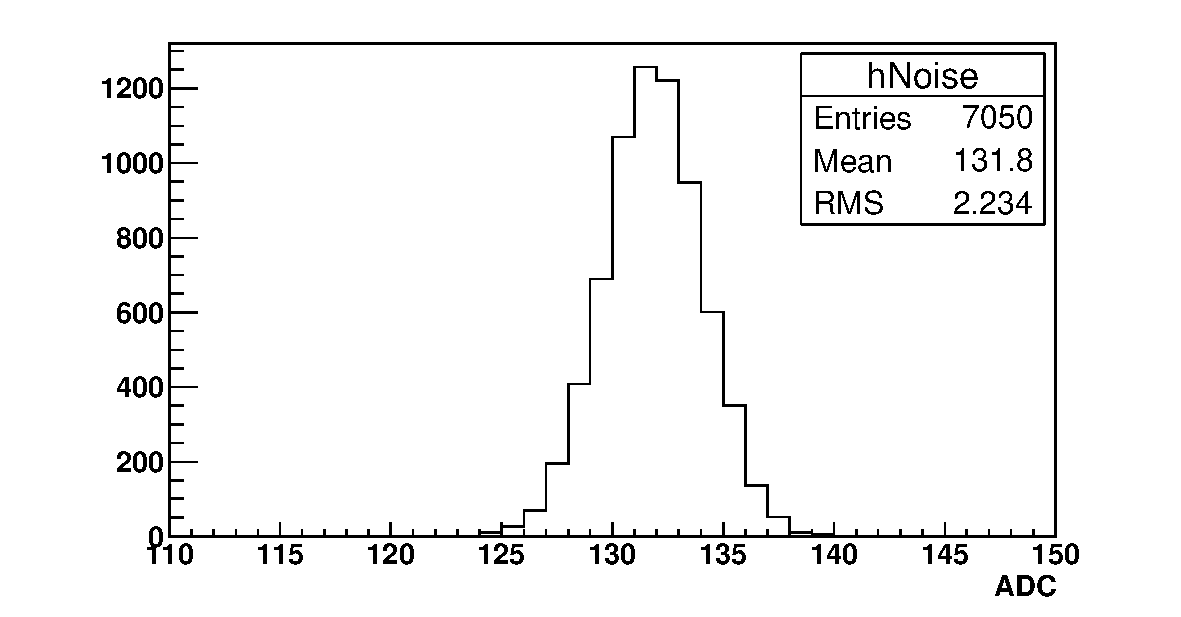
\includegraphics[width=\textwidth]{chapters/graphs/GainVarsMeas/LL_m04_2016-06-11/example_NoiseHist1.pdf}
\caption{Standard HV}
\end{subfigure}
\vspace{3mm}
\begin{subfigure}[b]{0.95\textwidth}
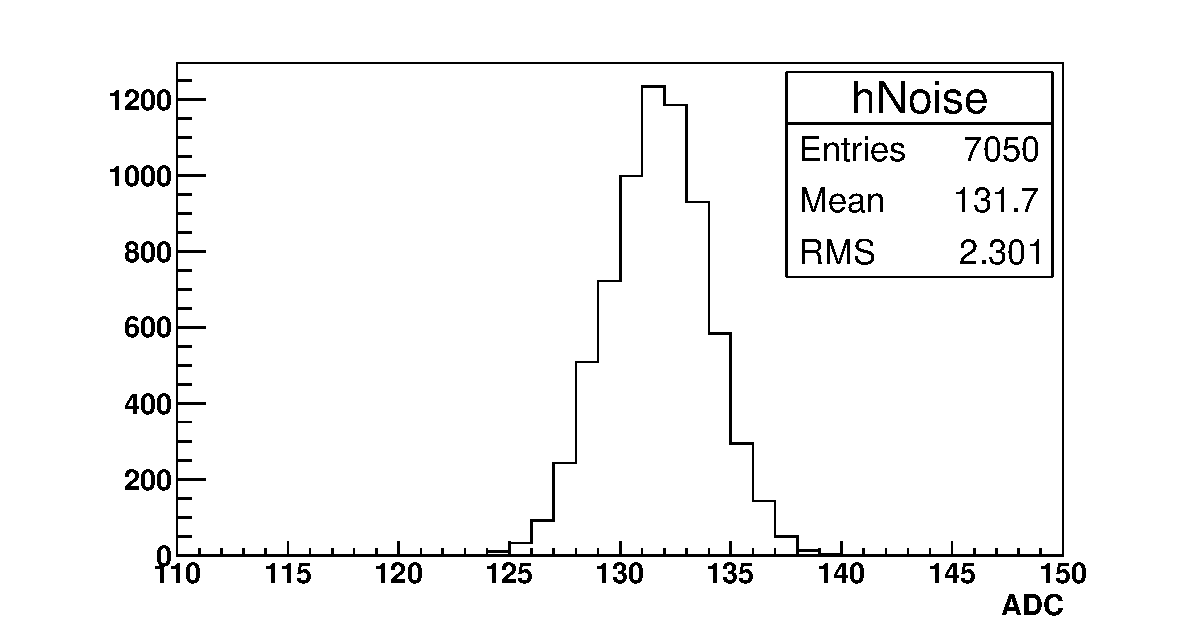
\includegraphics[width=\textwidth]{chapters/graphs/GainVarsMeas/LL_m04_2016-06-11/example_NoiseHist2.pdf}
\caption{Lower HV}
\end{subfigure}
\caption{Sample of the observed electronic noise observed for a single pixel within Los Leones telescope 4. Electronic noise outside of the PMT so will be the same separate from the HV setting across the PMT.}
\end{figure}

\section{Pairs Method}

For both standard and reduced voltage settings 50 sets of pulses are recorded for the CalA analysis. The pair method involves taking single CalA shots from standard and lower voltage settings and fitting an exponential to the signal. The fitted exponential is used to find the mean value at the top of the signal and the variance around the fit. For each pixel 50 values for the Gain Variance ratio is found and this is repeated for the 440 pixels within the FD telescope.

Fig. \ref{fig:CalAMeanADC_Pairs} shows the average ADC count found across a camera for a FD telescope. The pattern follow how the camera is illuminated by the LED pointing at the camera. It shows that the spot is brightness in the middle and the intensity drops off towards the edges \textbf{need to add in diagram of labelled pixel no. across a FD camera}. There are uncertainties on the averages but are smaller then the displayed points. The variance measured in Fig. \ref{fig:CalAVarsADC_Pairs} shows an expected pattern too. The variance is proportional to the mean and is expected to follow a similar shape. This will not be exact but a good indicator of whether the variance was calculated correctly.

\begin{figure} % Mean Plot
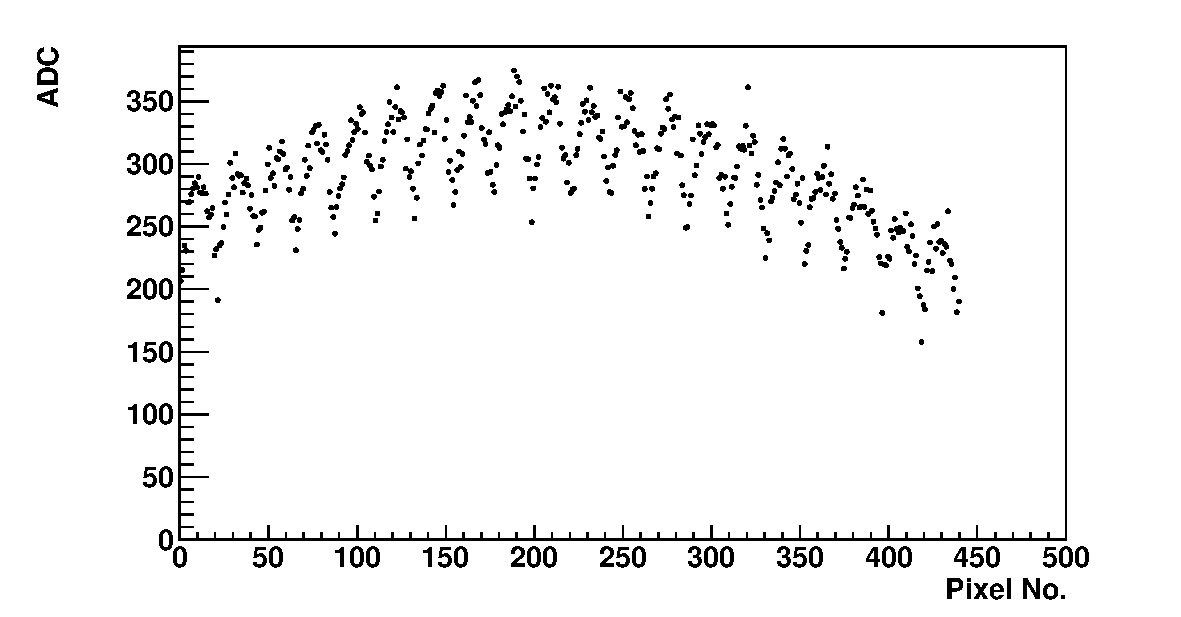
\includegraphics[width=\textwidth]{chapters/graphs/GainVarsMeas/LL_m04_2016-06-11/Set0and2/meanHist_StandHV_Pairs_set0and2.pdf}
\caption{Mean measured at Standard HV for Los Leones Mirror 4. CalA data taken on the 11-06-2016.}
\vspace{3mm}
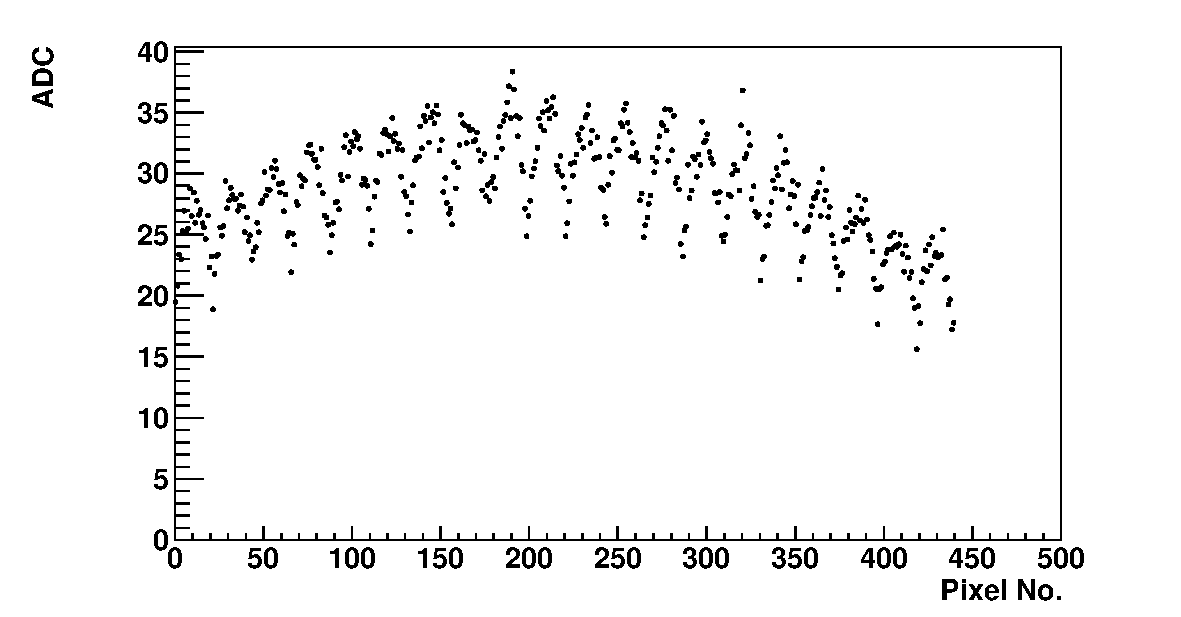
\includegraphics[width=\textwidth]{chapters/graphs/GainVarsMeas/LL_m04_2016-06-11/Set0and2/meanHist_LowHV_Pairs_set0and2.pdf}
\caption{Mean measured at Lower HV for Los Leones Mirror 4. CalA data taken on the 11-06-2016.} \label{fig:CalAMeanADC_Pairs}
\end{figure}

\begin{figure} % Variance Plot
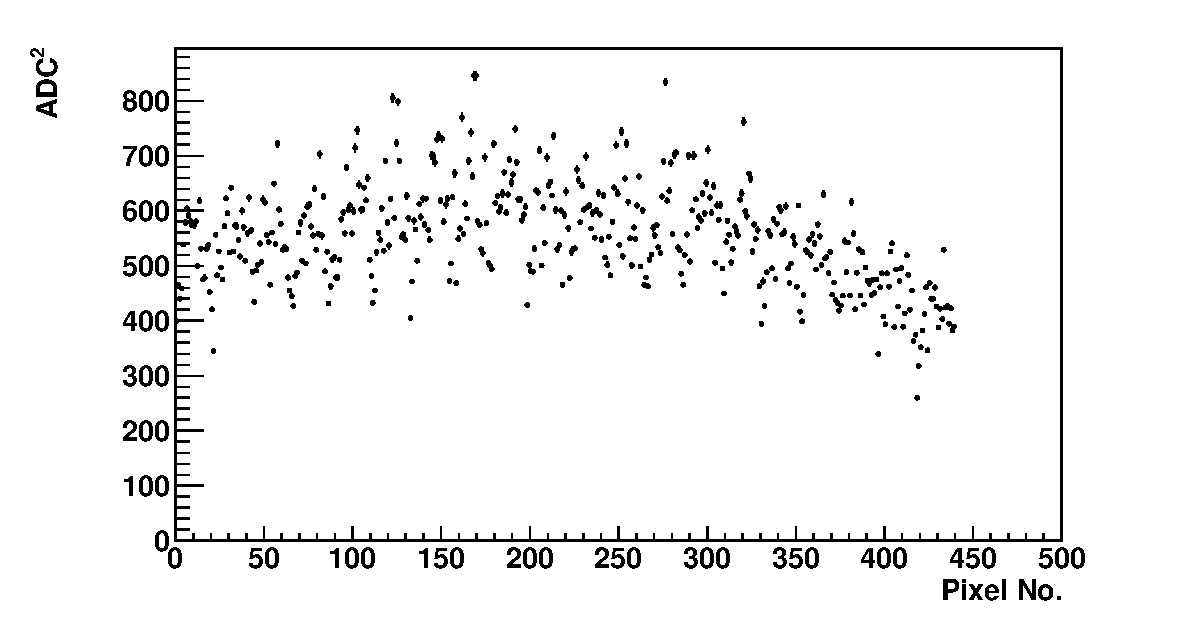
\includegraphics[width=\textwidth]{chapters/graphs/GainVarsMeas/LL_m04_2016-06-11/Set0and2/varianceHist_StandHV_Pairs_set0and2.pdf}
\caption{Variance measured at Standard HV for Los Leones Mirror 4. CalA data taken on the 11-06-2016.}
\vspace{3mm}
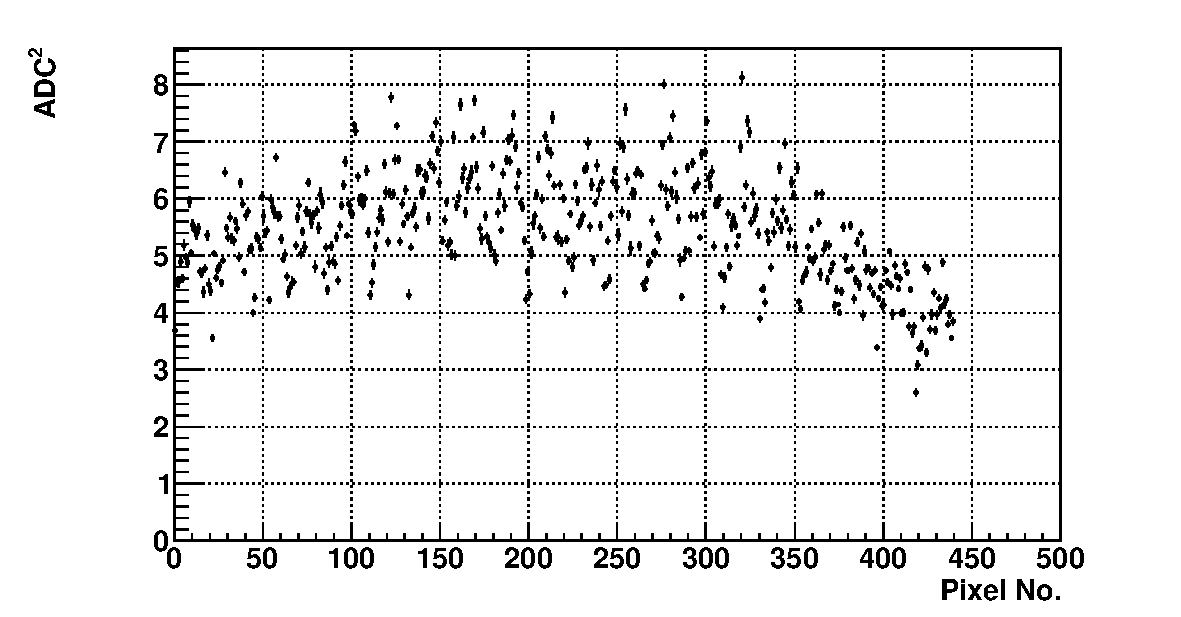
\includegraphics[width=\textwidth]{chapters/graphs/GainVarsMeas/LL_m04_2016-06-11/Set0and2/varianceHist_LowHV_Pairs_set0and2.pdf}
\caption{Varaince measured at Lower HV for Los Leones Mirror 4. CalA data taken on the 11-06-2016.} \label{fig:CalAVarsADC_Pairs}
\end{figure}

\subsection{Results}

Fig. \ref{fig:GainVarsRatio_Hist_PairsEx} and Fig. \ref{fig:GainVarsRatioVsPixel_PairsEx} shows a demonstration of using the Pairs Method to calculate the Gain Variance Ratio. The CalA data used was taken on the night of the 11-06-2016 by Los Leones Mirror 4. The mean value in Fig. \ref{fig:GainVarsRatio_Hist_PairsEx} shows a 3.7\% change in the ratio which translate to a 10\% change in the actual value of the PMT gain variance.

Fig. \ref{fig:GainVarsRatioVsPixel_PairsEx} shows the gain variance ratio measured per pixel. There can be seen no major structure or pattern. This is desired as the Gain variance is tired to individual PMTs and it would not be a great sign if the ratio followed a pattern like what was seen for the means and variances.

\begin{figure} % Gain Variance Plot
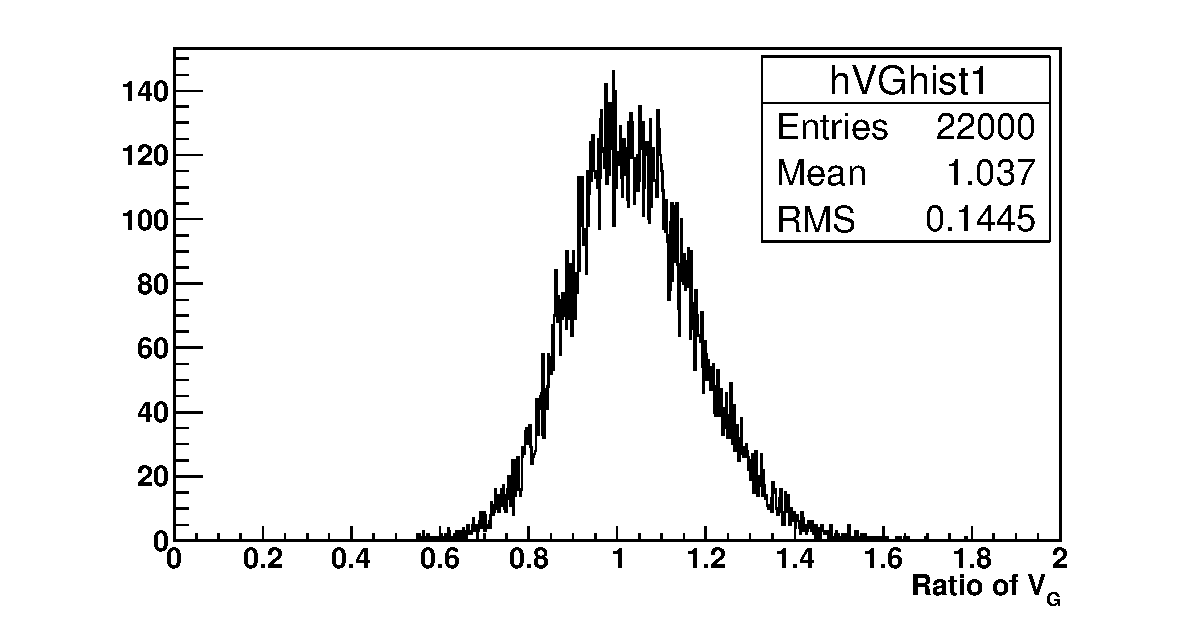
\includegraphics[width=\textwidth]{chapters/graphs/GainVarsMeas/LL_m04_2016-06-11/Set0and2/GainVairanceHist_Pairs.pdf}
\caption{Histogram of the all the pairs methods for Los Leones Mirror 4. CalA data was taken on the 11/06/2016 at both Standard and Lower gain settings. There are 50 traces for each of the 440 pixels recorded at both gain settings. } \label{fig:GainVarsRatio_Hist_PairsEx}
\vspace{3mm}
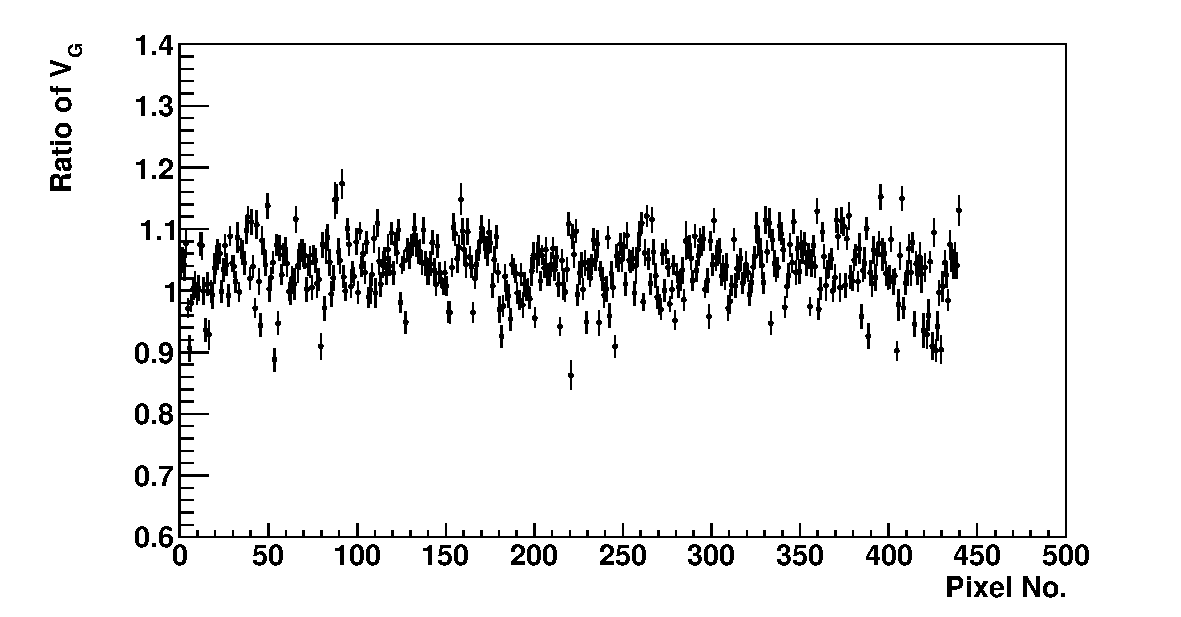
\includegraphics[width=\textwidth]{chapters/graphs/GainVarsMeas/LL_m04_2016-06-11/Set0and2/GainVars_Vs_Pixel_GainVariance_Pairs_Set0and2.pdf}
\caption{} \label{fig:GainVarsRatioVsPixel_PairsEx}
\end{figure}

\section{Averaging Sets of Traces Method}

Instead of calculating the Gain Variance ratio on pairs of CalA traces then finding an average value the 50 traces for each set are stacked. This forms an average trace consisting of the 50 traces. To find the mean and variances of the noise a linear line of form f(x) = x is fitted to the first 140 bins. the fitted x is used as the mean and the variance is calculated around this value. Next an exponential is fitted to the signal. The value of the fit at the top of the signal is used as the mean while the variance is calculated around the fitted exponential.  

\begin{figure} % Mean Plot
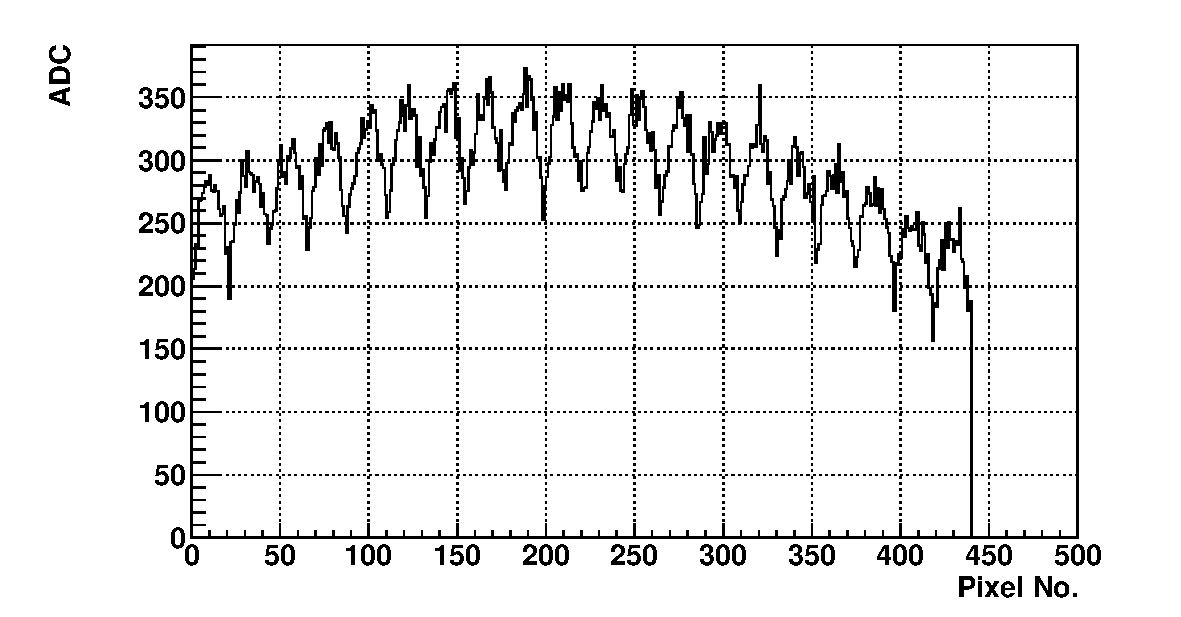
\includegraphics[width=\textwidth]{chapters/graphs/GainVarsMeas/LL_m04_2016-06-11/Set0and2/meanHist_StandHV_Average_set0and2.pdf}
\caption{}\label{fig:MeanVsPixel_StandardHV_Average}
\vspace{3mm}
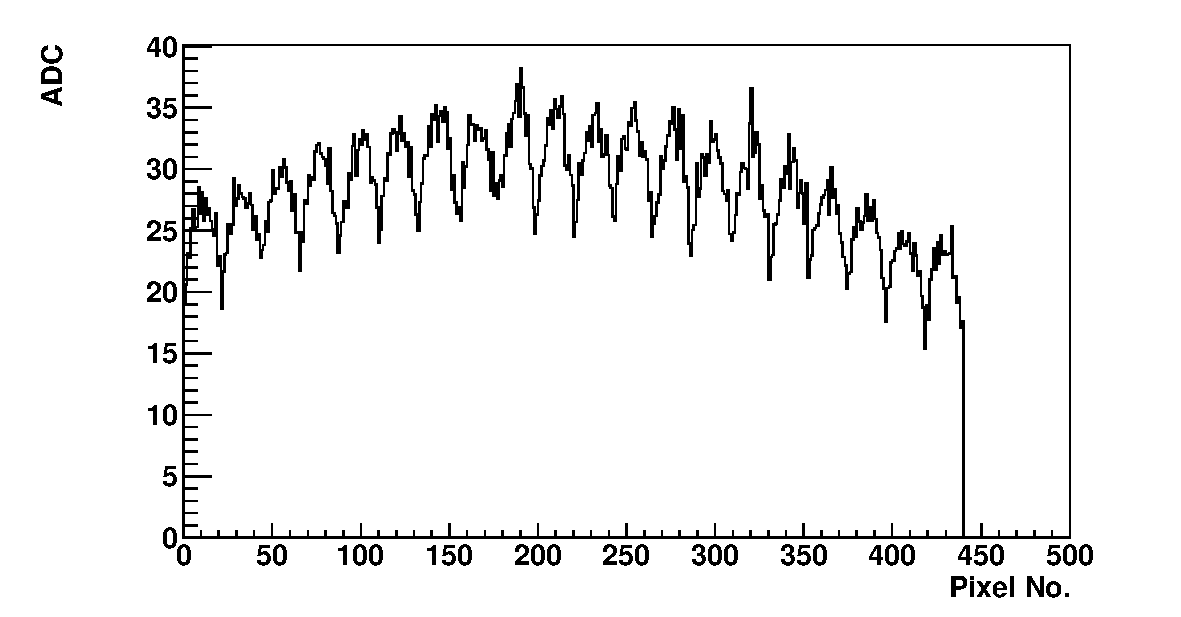
\includegraphics[width=\textwidth]{chapters/graphs/GainVarsMeas/LL_m04_2016-06-11/Set0and2/meanHist_LowHV_Average_set0and2.pdf}
\caption{}\label{fig:MeanVsPixel_LowerHV_Average}
\end{figure}

\begin{figure} % Variance Plot
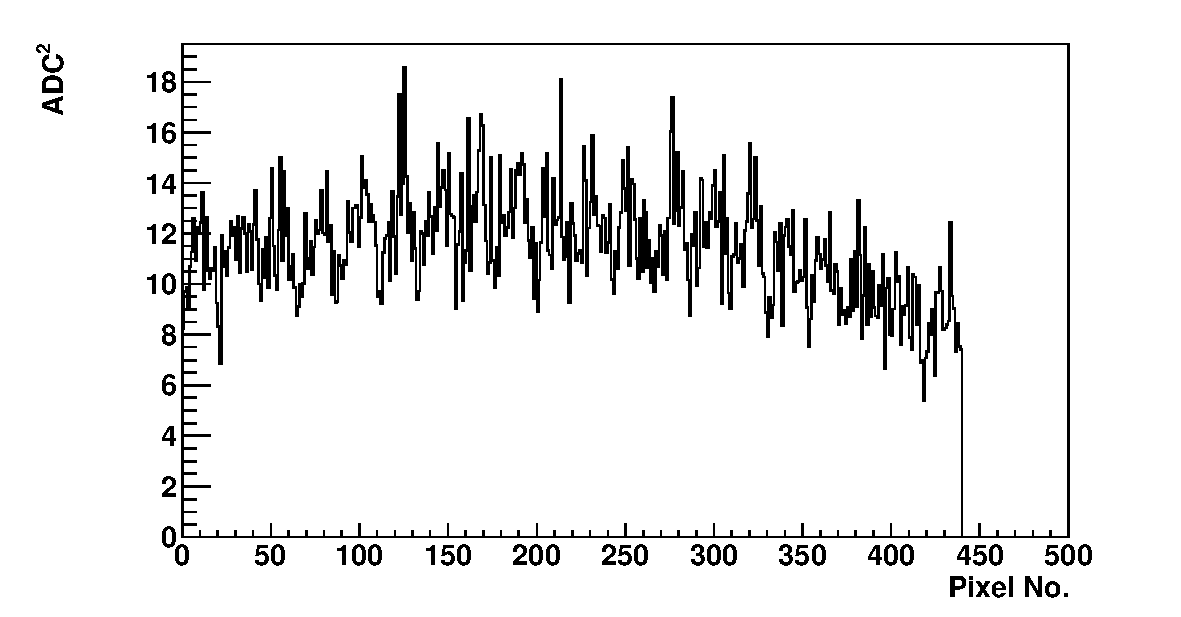
\includegraphics[width=\textwidth]{chapters/graphs/GainVarsMeas/LL_m04_2016-06-11/Set0and2/varianceHist_StandHV_Average_set0and2.pdf}
\caption{}\label{fig:VarsVsPixel_StandardHV_Average}
\vspace{3mm}
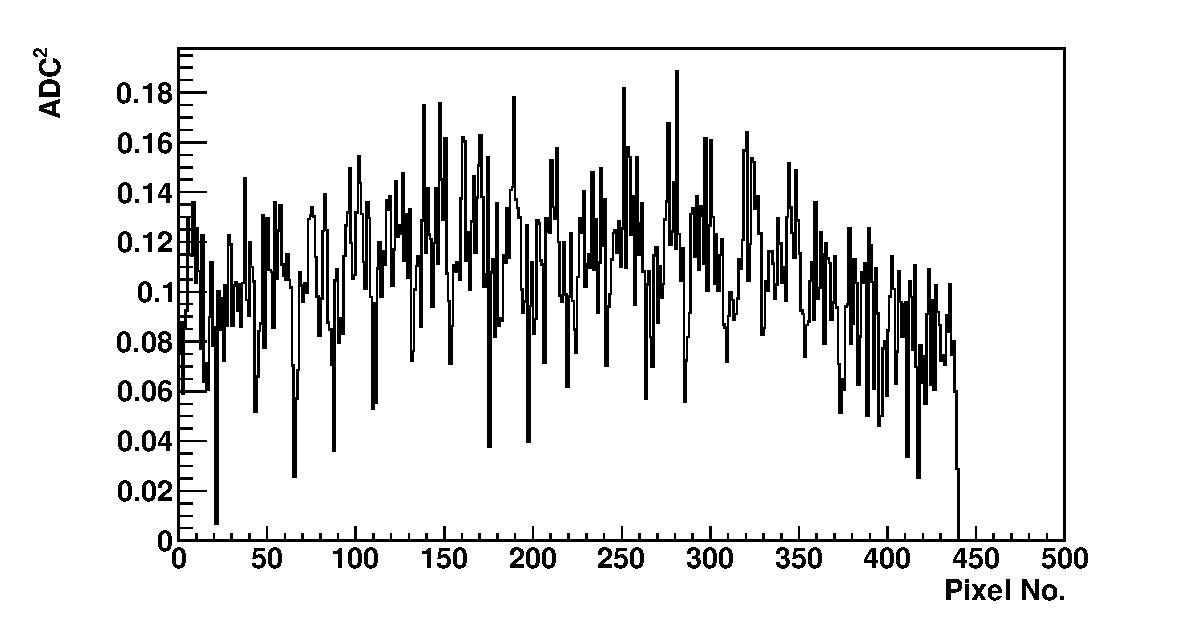
\includegraphics[width=\textwidth]{chapters/graphs/GainVarsMeas/LL_m04_2016-06-11/Set0and2/varianceHist_LowHV_Average_set0and2.pdf}
\caption{}\label{fig:VarsVsPixel_LowerHV_Average}
\end{figure}

\subsection{Results}

There is a larger spread in the histogram of calculated Gain Variance ratio then when the Pairs Method was employed. One good property is that no visible structure or pattern can be seen. There are definitely some extreme values of the ratio measured. To see what could cause the large outliers I had a look at the reduced chi-square of the fitted function to the noise and signal. There was no obvious problems when the looking at the chi-squares as a function of pixel number for the signal. Examples are shown in Fig. \ref{fig:Chi2VsPixel_Signal_StandHV_Average} and Fig. \ref{fig:Chi2VsPixel_Signal_LowerHV_Average}. Examining the reduced chi-square of the fits to the noise it was seen that there was some large values. This was shown in Fig. \ref{fig:Chi2VsPixel_Noise_StandHV_Average} and Fig. \ref{fig:Chi2VsPixel_Noise_LowerHV_Average}. What was causing these weird fits was one or more of the noise bins having a larger deviation then expected from the measured average. \textbf{Add in plot showing off this behaviour}. This led to the process of investigating whether Least Trimmed Squares would be useful.

\begin{figure} % Gain Variance Plot
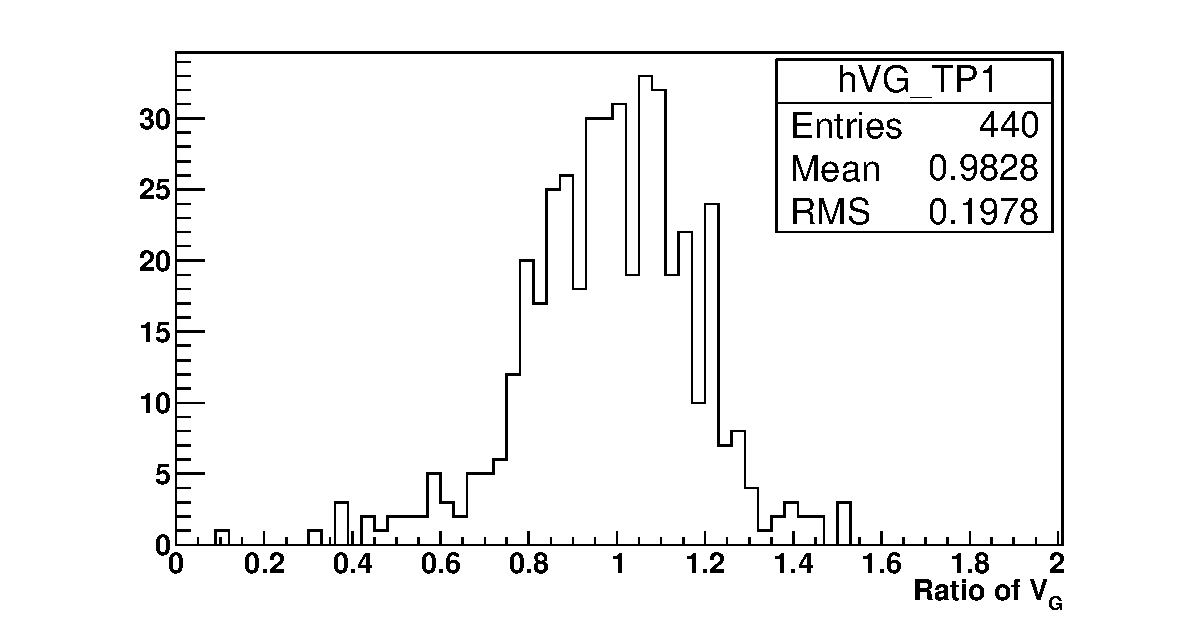
\includegraphics[width=\textwidth]{chapters/graphs/GainVarsMeas/LL_m04_2016-06-11/Set0and2/GainVairanceHist_Average_Method1.pdf}
\caption{}\label{fig:GainVarsRatioHist_Average}
\vspace{3mm}
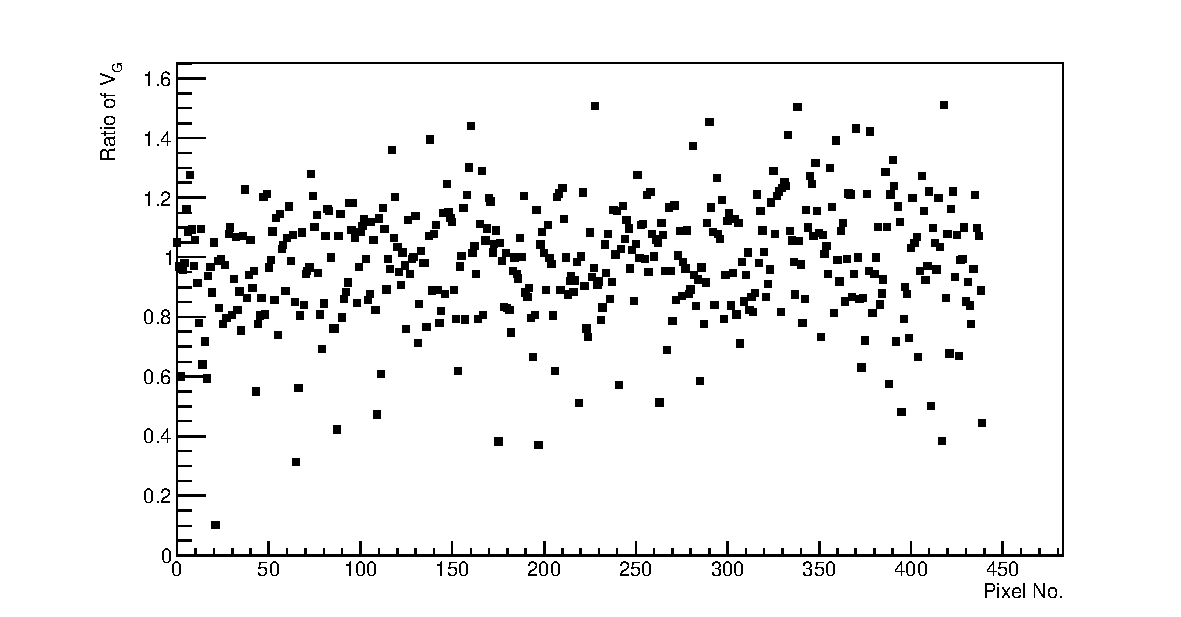
\includegraphics[width=\textwidth]{chapters/graphs/GainVarsMeas/LL_m04_2016-06-11/Set0and2/GainVars_Vs_Pixel_GainVariance_Average_Method1_Set0and2.pdf}
\caption{}\label{fig:GainsVarsRatioVsPixel_Average}
\end{figure}

\begin{figure}% Signal Chi2
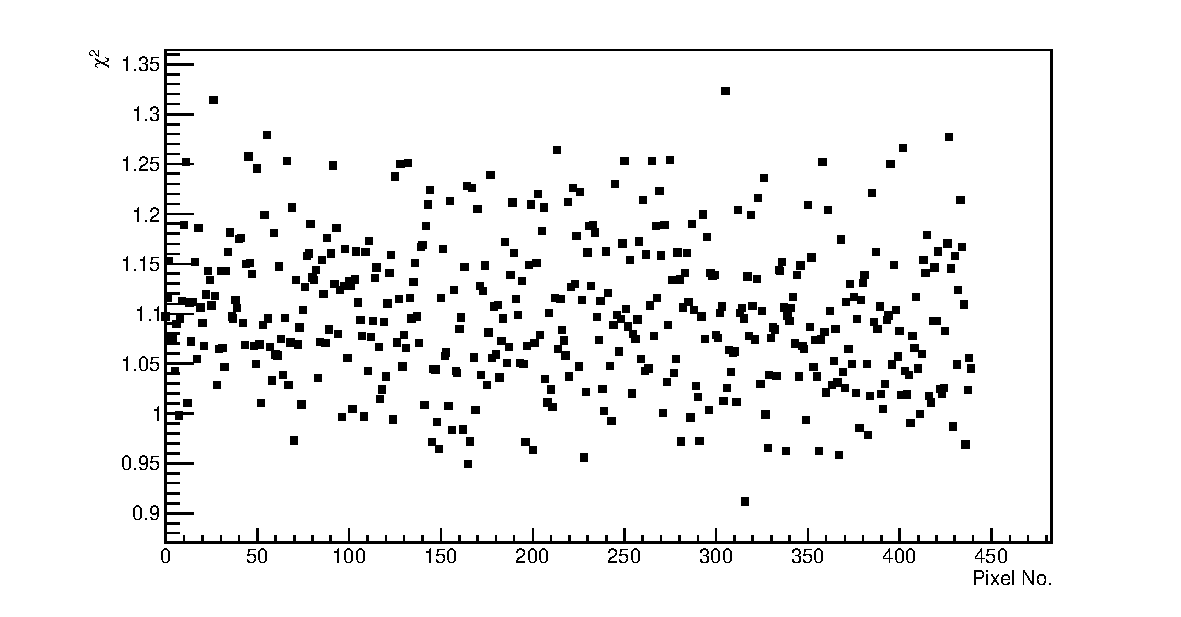
\includegraphics[width=\textwidth]{chapters/graphs/GainVarsMeas/LL_m04_2016-06-11/Set0and2/Chi2_AverageMethod_Signal_StandHV.pdf}
\caption{Reduced Chi-square for fitted exponential on the signal for CalA events measured at Standard HV.}\label{fig:Chi2VsPixel_Signal_StandHV_Average}
\vspace{3mm}
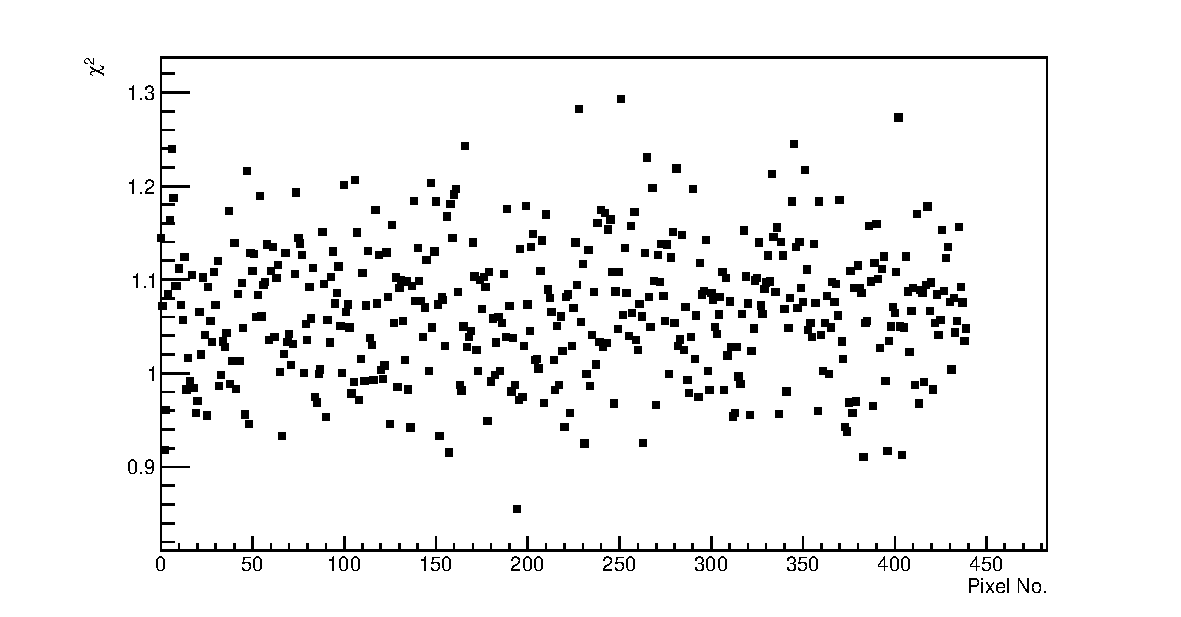
\includegraphics[width=\textwidth]{chapters/graphs/GainVarsMeas/LL_m04_2016-06-11/Set0and2/Chi2_AverageMethod_Signal_LowHV.pdf}
\caption{Reduced Chi-square for fitted exponential on the signal for CalA events measured at Lower HV.}\label{fig:Chi2VsPixel_Signal_LowerHV_Average}
\end{figure}

\begin{figure}% Noise Chi2
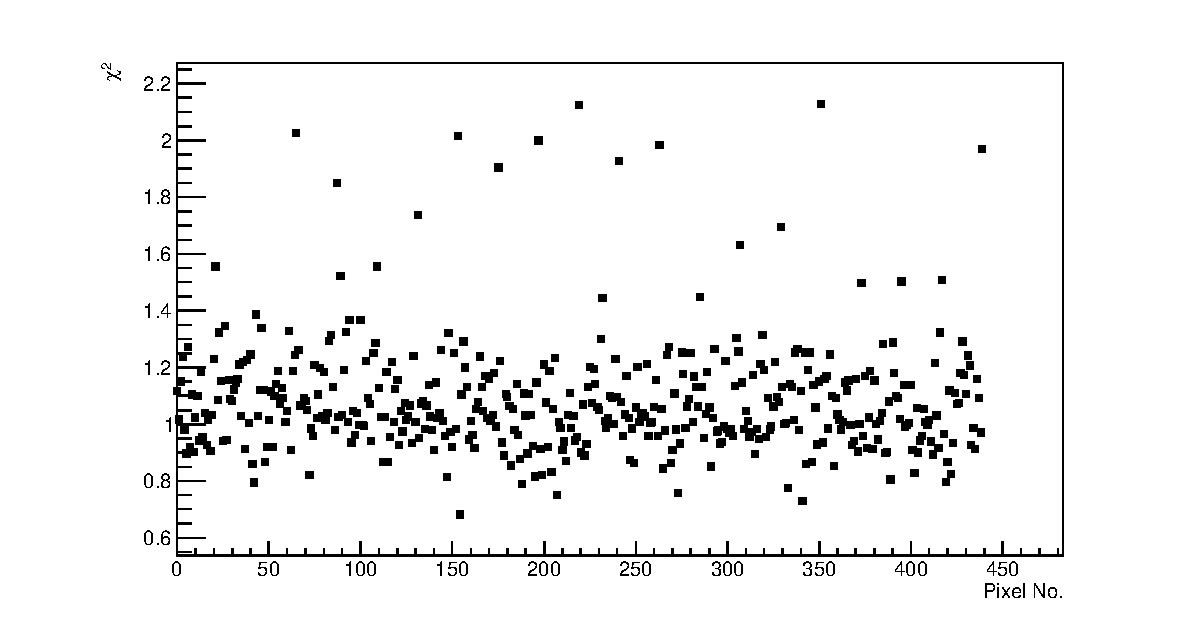
\includegraphics[width=\textwidth]{chapters/graphs/GainVarsMeas/LL_m04_2016-06-11/Set0and2/Chi2_AverageMethod_Noise_StandHV.pdf}
\caption{Reduced Chi-square for fitted line on the signal for CalA events measured at Standard HV.}\label{fig:Chi2VsPixel_Noise_StandHV_Average}
\vspace{3mm}
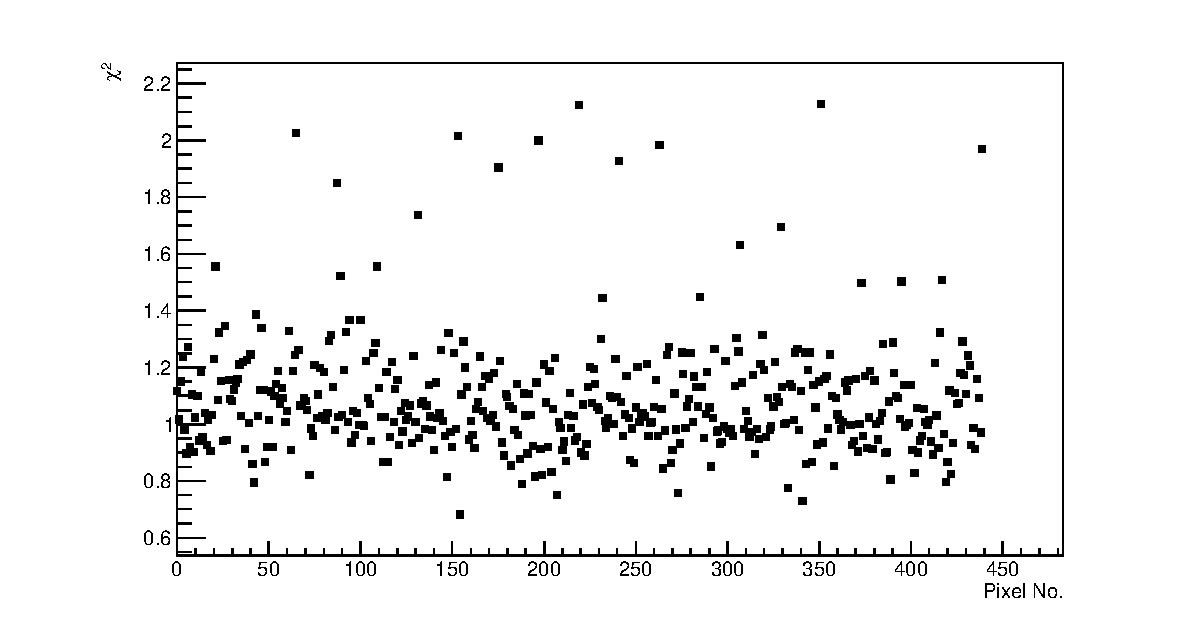
\includegraphics[width=\textwidth]{chapters/graphs/GainVarsMeas/LL_m04_2016-06-11/Set0and2/Chi2_AverageMethod_Noise_LowHV.pdf}
\caption{Reduced Chi-square for fitted line on the signal for CalA events measured at Lower HV.}\label{fig:Chi2VsPixel_Noise_LowerHV_Average}
\end{figure}

\section{Result of Averaging Sets of Traces Method with Least Trimmed Squares}

Least Trimmed Square is the method that involves removing points that have the greatest sigma away from an initial fit. A point is removed one at a time with the fit repeated and the reduced chi-square checked. This method is repeated until the reduced chi-square is below a threshold.


\begin{figure} % Gain Variance Plot
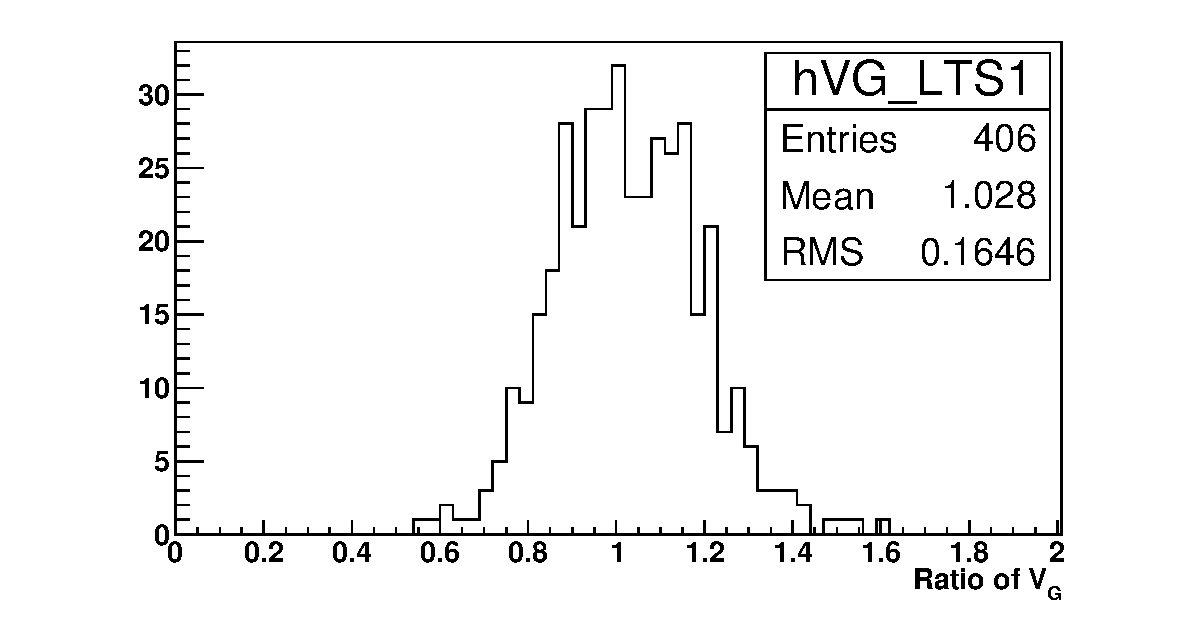
\includegraphics[width=\textwidth]{chapters/graphs/GainVarsMeas/LL_m04_2016-06-11/Set0and2/GainVairanceHist_Average_LTS.pdf}
\caption{}
\vspace{3mm}
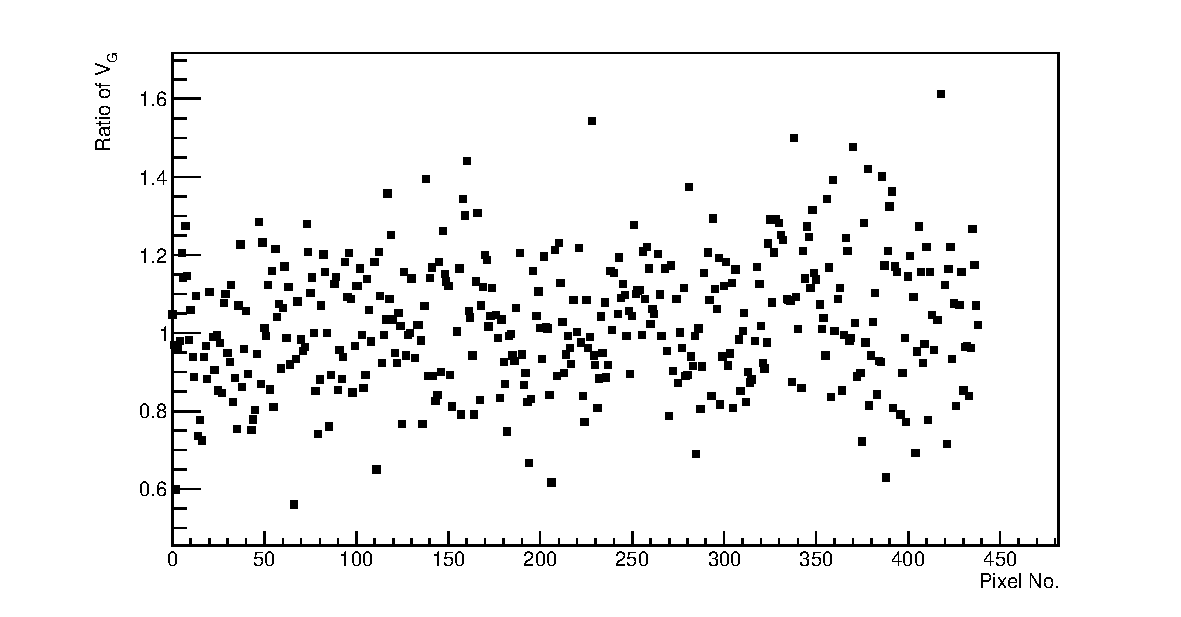
\includegraphics[width=\textwidth]{chapters/graphs/GainVarsMeas/LL_m04_2016-06-11/Set0and2/GainVars_Vs_Pixel_GainVariance_AverageLTS_Set0and2.pdf}
\caption{}
\end{figure}

\section{Result of Averaging Sets of Traces Method using Noise Distribution}

\begin{figure} % Gain Variance Plot
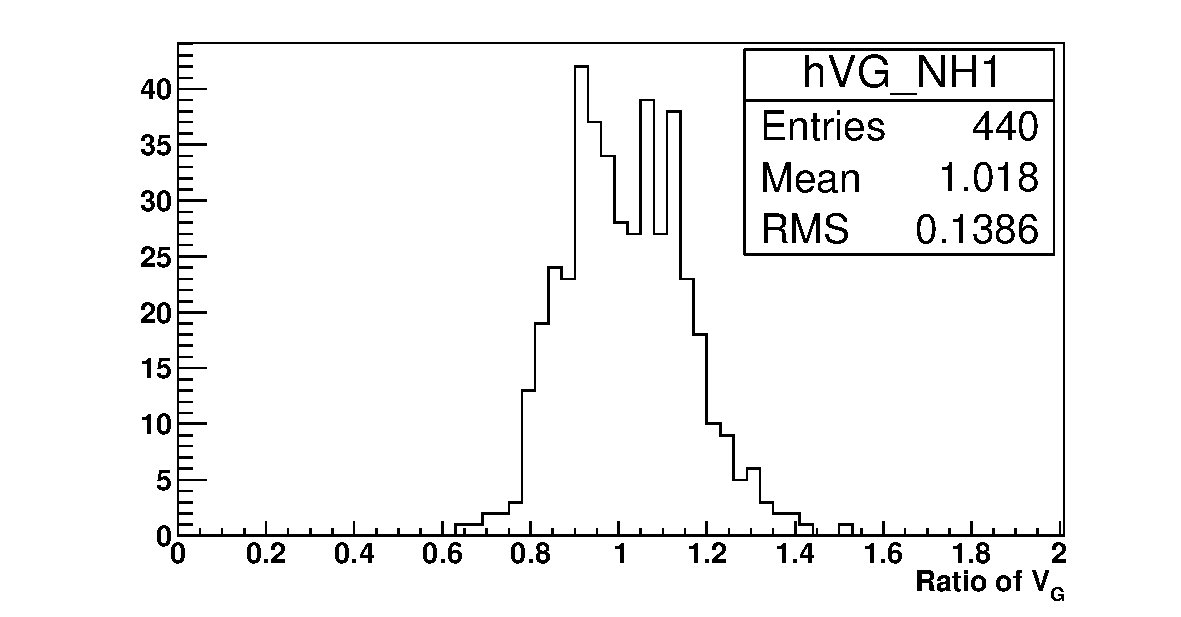
\includegraphics[width=\textwidth]{chapters/graphs/GainVarsMeas/LL_m04_2016-06-11/Set0and2/GainVairanceHist_Average_Method2.pdf}
\caption{}
\vspace{3mm}
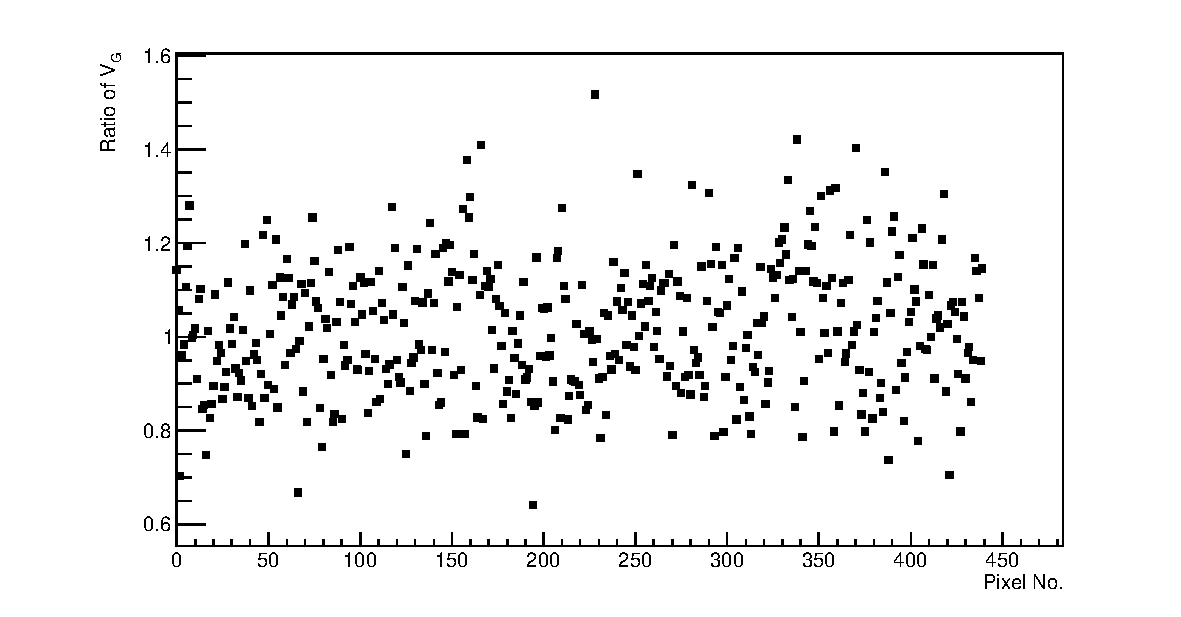
\includegraphics[width=\textwidth]{chapters/graphs/GainVarsMeas/LL_m04_2016-06-11/Set0and2/GainVars_Vs_Pixel_GainVariance_Average_Method2_Set0and2.pdf}
\caption{}
\end{figure}

\section{Attempts to measure Gain Variance directly in the Lab}
\chapter{Laboratory Simulation of FD shift}\label{Ch:LabPMTshift}

Laboratory Simulation of FD shift under differing NSB levels.
\begin{itemize}
\item Measurements for both 900V and 600V (900V used as baseline)
\item Different length shifts
\item Changing NSB
\item measuring how the relevant Gain changes throughout a run
\end{itemize}
\chapter[Evaluation of Cloud Cuts on Auger Event Data]{\centering Evaluation of Cloud Cuts on Auger Event Data \\}\label{Ch:CloudCuts}

This is an initial look into the effectiveness of the cloud cuts on reconstructed Fluorescence Detector events from 2004 to 2018. The set was restricted to Golden Hybrid events which are detected events that have both an FD and SD reconstruction available. The cloud cut described here are part of a series of quality cuts used to produce datasets for the ICRC 2019 conference. These series of quality cuts are used produce standardised datasets across the collaboration. I investigated the effects of removing the cloud cut from this series of quality cuts and quantify the effects of removal through the Elongation Rate and the Xmax distributions. Within this chapter I show the series of quality cuts used for this analysis.

%The cloud cut is just one of a series of quality cuts that are used to create sets of event that are ready for further analysis. The list  I investigated the effects of removing the cloud cut from this list of quality cuts and quantify the effects of removal through the Elongation Rate and the Xmax distributions. This list includes cuts to remove events within known bad data taking periods, cuts on aerosol levels, event quality etc. 

This investigation was done to quantify the effects that the cloud cuts had on the data set. A question had been raised about whether the quality cuts on fitted values, constraining the  $\chi^2$ and requiring events without large gaps were doing the same job as the cloud cuts. There is a lot of uncertainty about whether a detected cloud had impacted each event due to the time spacing of atmospheric measurements. The timing can sometimes vary between 5 and 15 minutes when measurements are available or larger if  atmospheric data is missing. Another reason to see if the other quality cuts are doing a similar job as the cloud cut is to help when cloud measurements are unavailable. There are multiple different cloud detection sources but none are prefect. It would be great to have alternative that can cover the rare times when we do not have atmospheric cloud measurements.

It is important to know where clouds are located in relation to EAS events due to the different effects that clouds can have on the detected light profile by the FDs. If a cloud partially obscures the FD view of the event it can cause a gap in the profile or a cloud may be in the path of the development of the EAS event. In the first case a gap will cause the reconstruction of the energy of the event to be underestimated. In the second case a cloud within the path of development can amplify the amount of Cherenkov light scattered towards the FD which can in turn cause an overestimate of the reconstructed energy.

Cloud information has large uncertainty about quantities like cloud height, distance from telescopes and timing. The main uncertainty is due to time gaps between data taken of the atmosphere. Examples of this are that cloud camera scans are performed every 5 minutes. Since this a snapshot, a cloud could move quite a far distance within this time spacing and introduce a large uncertainty.

\section{Equipment used to monitor clouds above the array} \label{sec:MonitoringEquipment}



\begin{figure}[!t]
\begin{subfigure}[b]{0.3\textwidth}
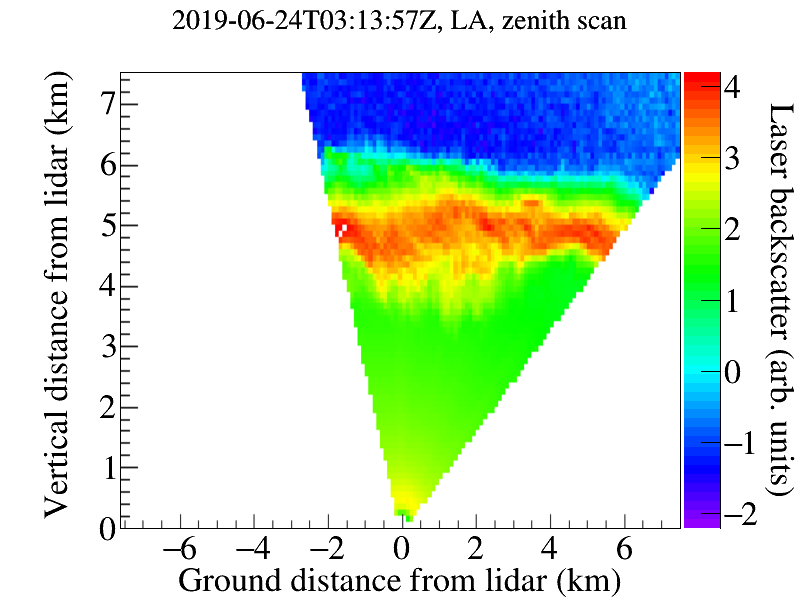
\includegraphics[width=\textwidth]{chapters/graphs/CloudFlags/lidar_scan.png}
\caption{} \label{subfig:liadr_scan}
\end{subfigure}
\begin{subfigure}[b]{0.3\textwidth}
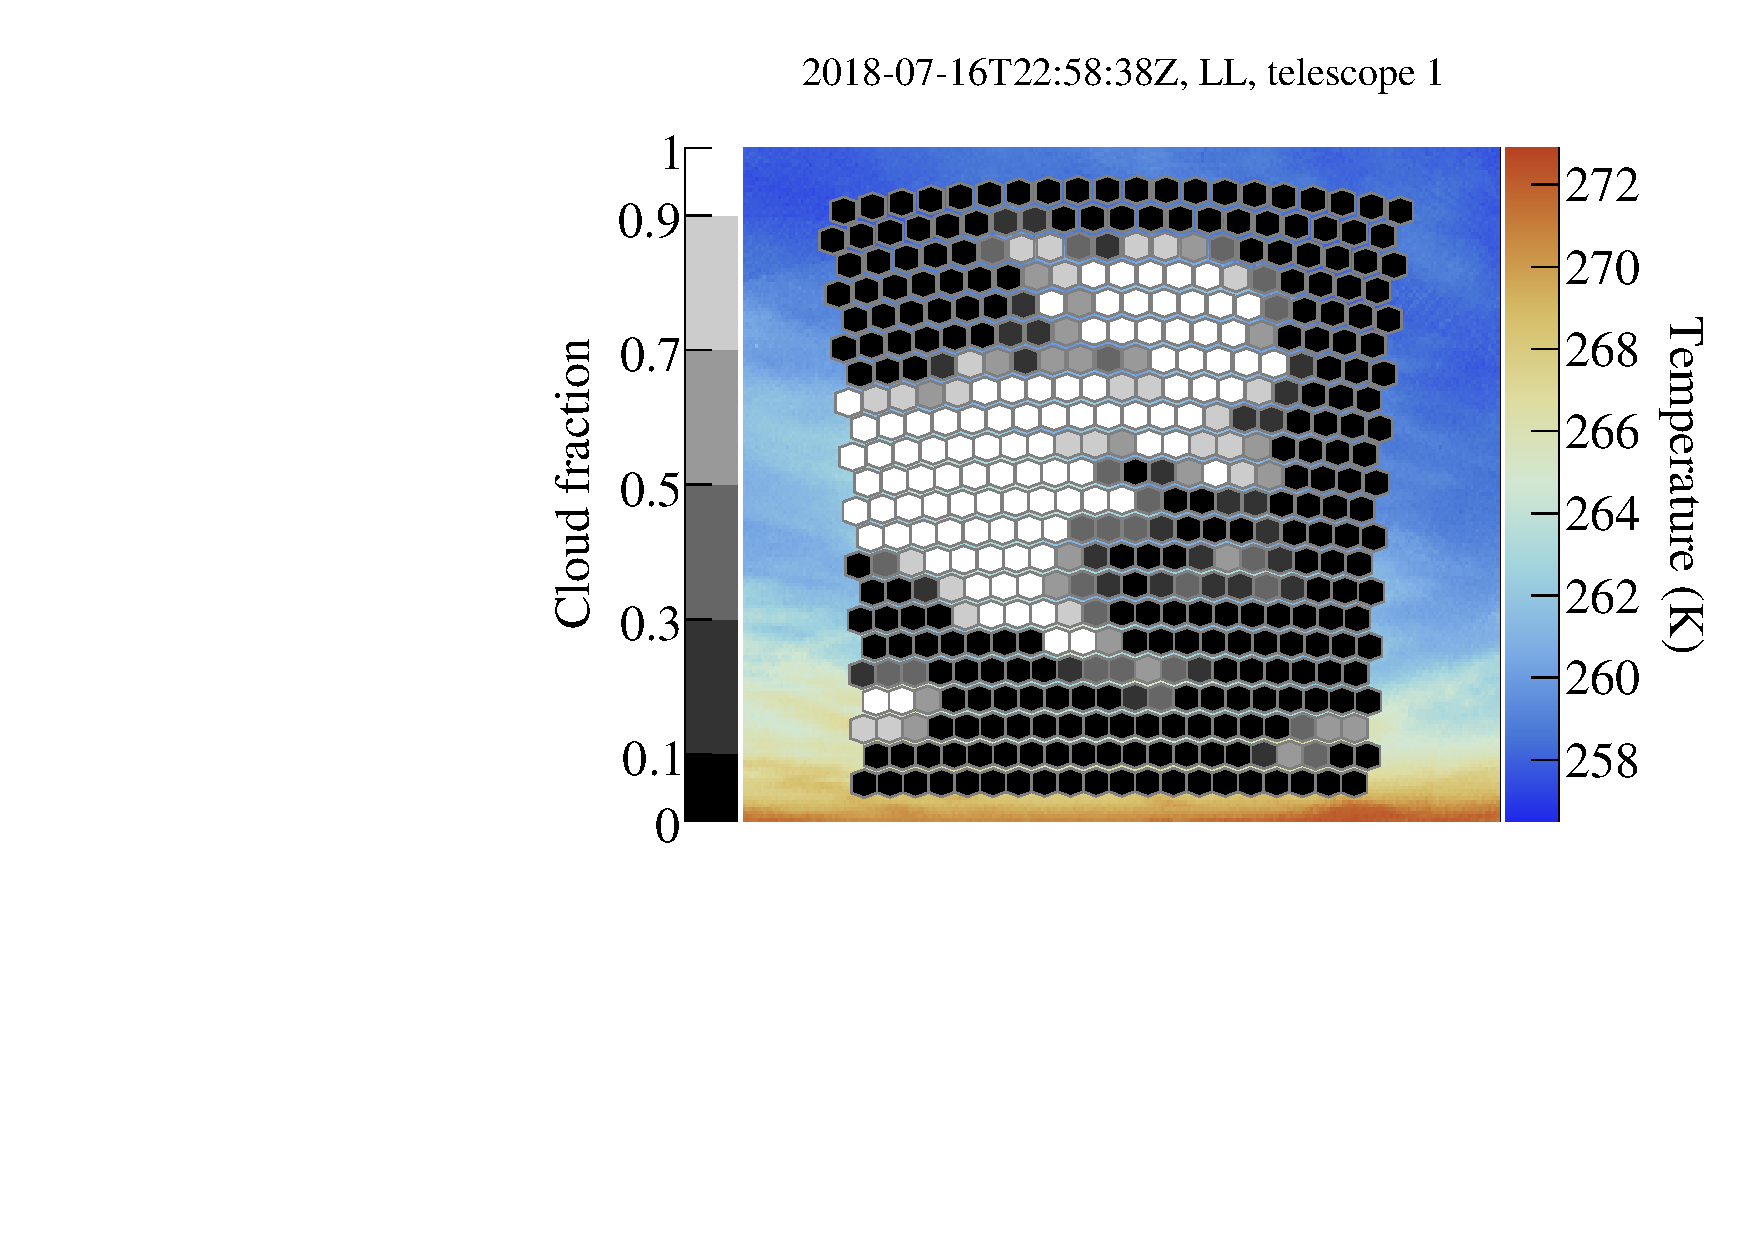
\includegraphics[width=\textwidth]{chapters/graphs/CloudFlags/ir_cloudfraction_pixels.pdf}
\caption{} \label{subfig:IR_cloudcam}
\end{subfigure}
\begin{subfigure}[b]{0.3\textwidth}
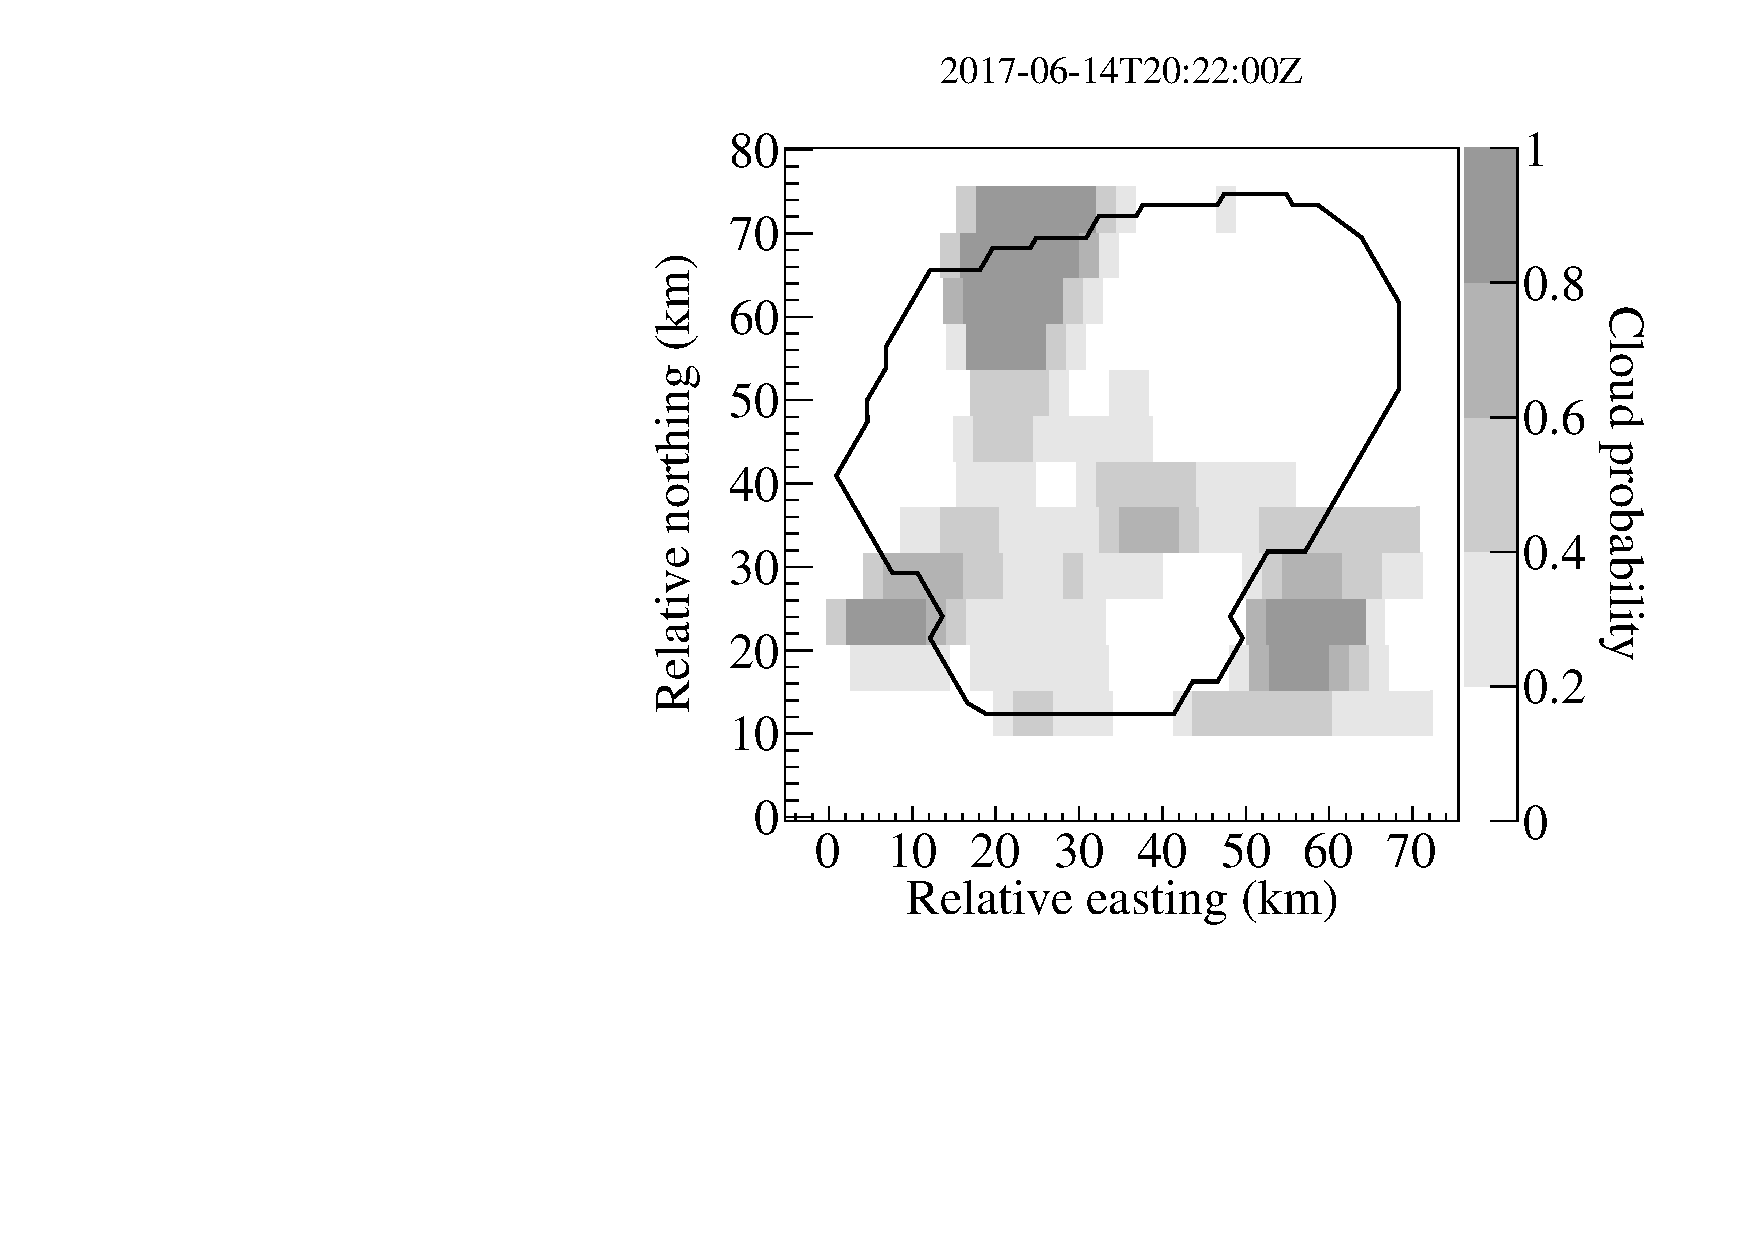
\includegraphics[width=\textwidth]{chapters/graphs/CloudFlags/ir_cloudprobability_map.pdf}
\caption{} \label{subfig:GOES}
\end{subfigure}
\caption{Examples of real data from (a) FD lidar scan, (b) cloud camera mask mapped to each pixel of a single FD telescope and (c) GOES cloud probability map covering the entire array.  Images provide by permission by V. Harvey.}
\end{figure}

There are multiple instruments used to monitor the cloud coverage across the array. These are a combination of collaboration run instruments specifically set-up to monitor atmospheric conditions within the array and externally run instruments that monitor broader atmospheric conditions that happen to include the array. The combination of instruments used to monitor clouds are the lidar system and infra-red cameras at each FD site, the Geostationary Operational Environmental Satellite (GOES) system, and the Central Laser Facility (CLF) and the eXtreme Laser Facility.

 
\subsection{Lidar System, Central Laser Facility and eXtreme Laser Facility}

There are three sets of lidar systems that are used to monitor the atmospheric conditions above the array. These sets are the monostatic elastic backscatter lidar deployed behind each of the FD telescope sites, the Central Laser Facility (CLF) and the eXtreme Laser Facility (XLF).

The monostatic elastic backscatter lidar is programmed to scan the sky above the FD field of view every 15 minutes. it works on the principle of measuring the time delay and magnitude of the returned signal to determine the distance and density of scattering centres. Both a minimum cloud base height (CBH) and percentage of overhead cloud coverage can be calculated. The overall CBH is an hourly average of all the 15 minute scans from all the FD sites. An example of a returned signal map is shown in Figure \ref{subfig:liadr_scan}. This example shows an overhead scan which indicates a localised cloud base height (CBH) of 4 km. The CBH and percentage of overhead cloud coverage is used when considering whether an event can be used in different analyses within Auger.


The CLF and the XLF's main purpose is to measure the atmospheric aerosol content but can be used to detect clouds either directly above the lasers or between the path of the laser and an FD site. A CBH can be determined for clouds detected directly above the laser or a lower limit can be determine if a cloud is detected between the laser and an FD site. The average CBH for an hour period is determined by the lowest CBH for any laser to FD pair measured within the hour.


\subsection{Infra-Red Cameras}

The main monitoring cloud system used is the infra-red cameras located on the roof of each of the FD sites. The cameras record light between 8 $\mu$m and 14 $\mu$m which measures clouds as warmer then the sky. The cloud cameras take images of the FoV of the FD eyes every 5 minutes while a full sky scan is performed every 15 minutes. The images within the FoV of the FD eyes are analysed to calculate a cloud fraction between 0\% and 100\% for each of the FD pixels. An example of the cloud mask being mapped to individual FD pixels is shown in Figure \ref{subfig:IR_cloudcam}. The pixels observing $\sim$ 5\textdegree \ elevation and below are not assigned a cloud fraction as observing clouds this close to the ground is difficult. The difficulty arises due to the fact that in IR the atmosphere becomes optically thick close to the horizon and the large present of water vapour close to the ground. When an event is reconstructed, the cloud fraction of each FD pixel that observed the EAS event is queried.

\subsection{Geostationary Operational Environmental Satellite (GOES) system}

The Geostationary Operational Environmental Satellite system (GOES) is operated by the United States National Oceanic and Atmospheric Administration. Auger uses the raw data that is publicly available and has created an algorithm to convert the aerial measurements across four IR bands to produce a cloud probability map every 30 minutes. An example of a GOES cloud probability map is shown in Figure \ref{subfig:GOES}. Each block represents a satellite pixel that covers an 2.4 km by 5.5 km area on the ground.

\section{Cloud Cuts employed on Auger data}

\begin{figure}[!t]
\centering
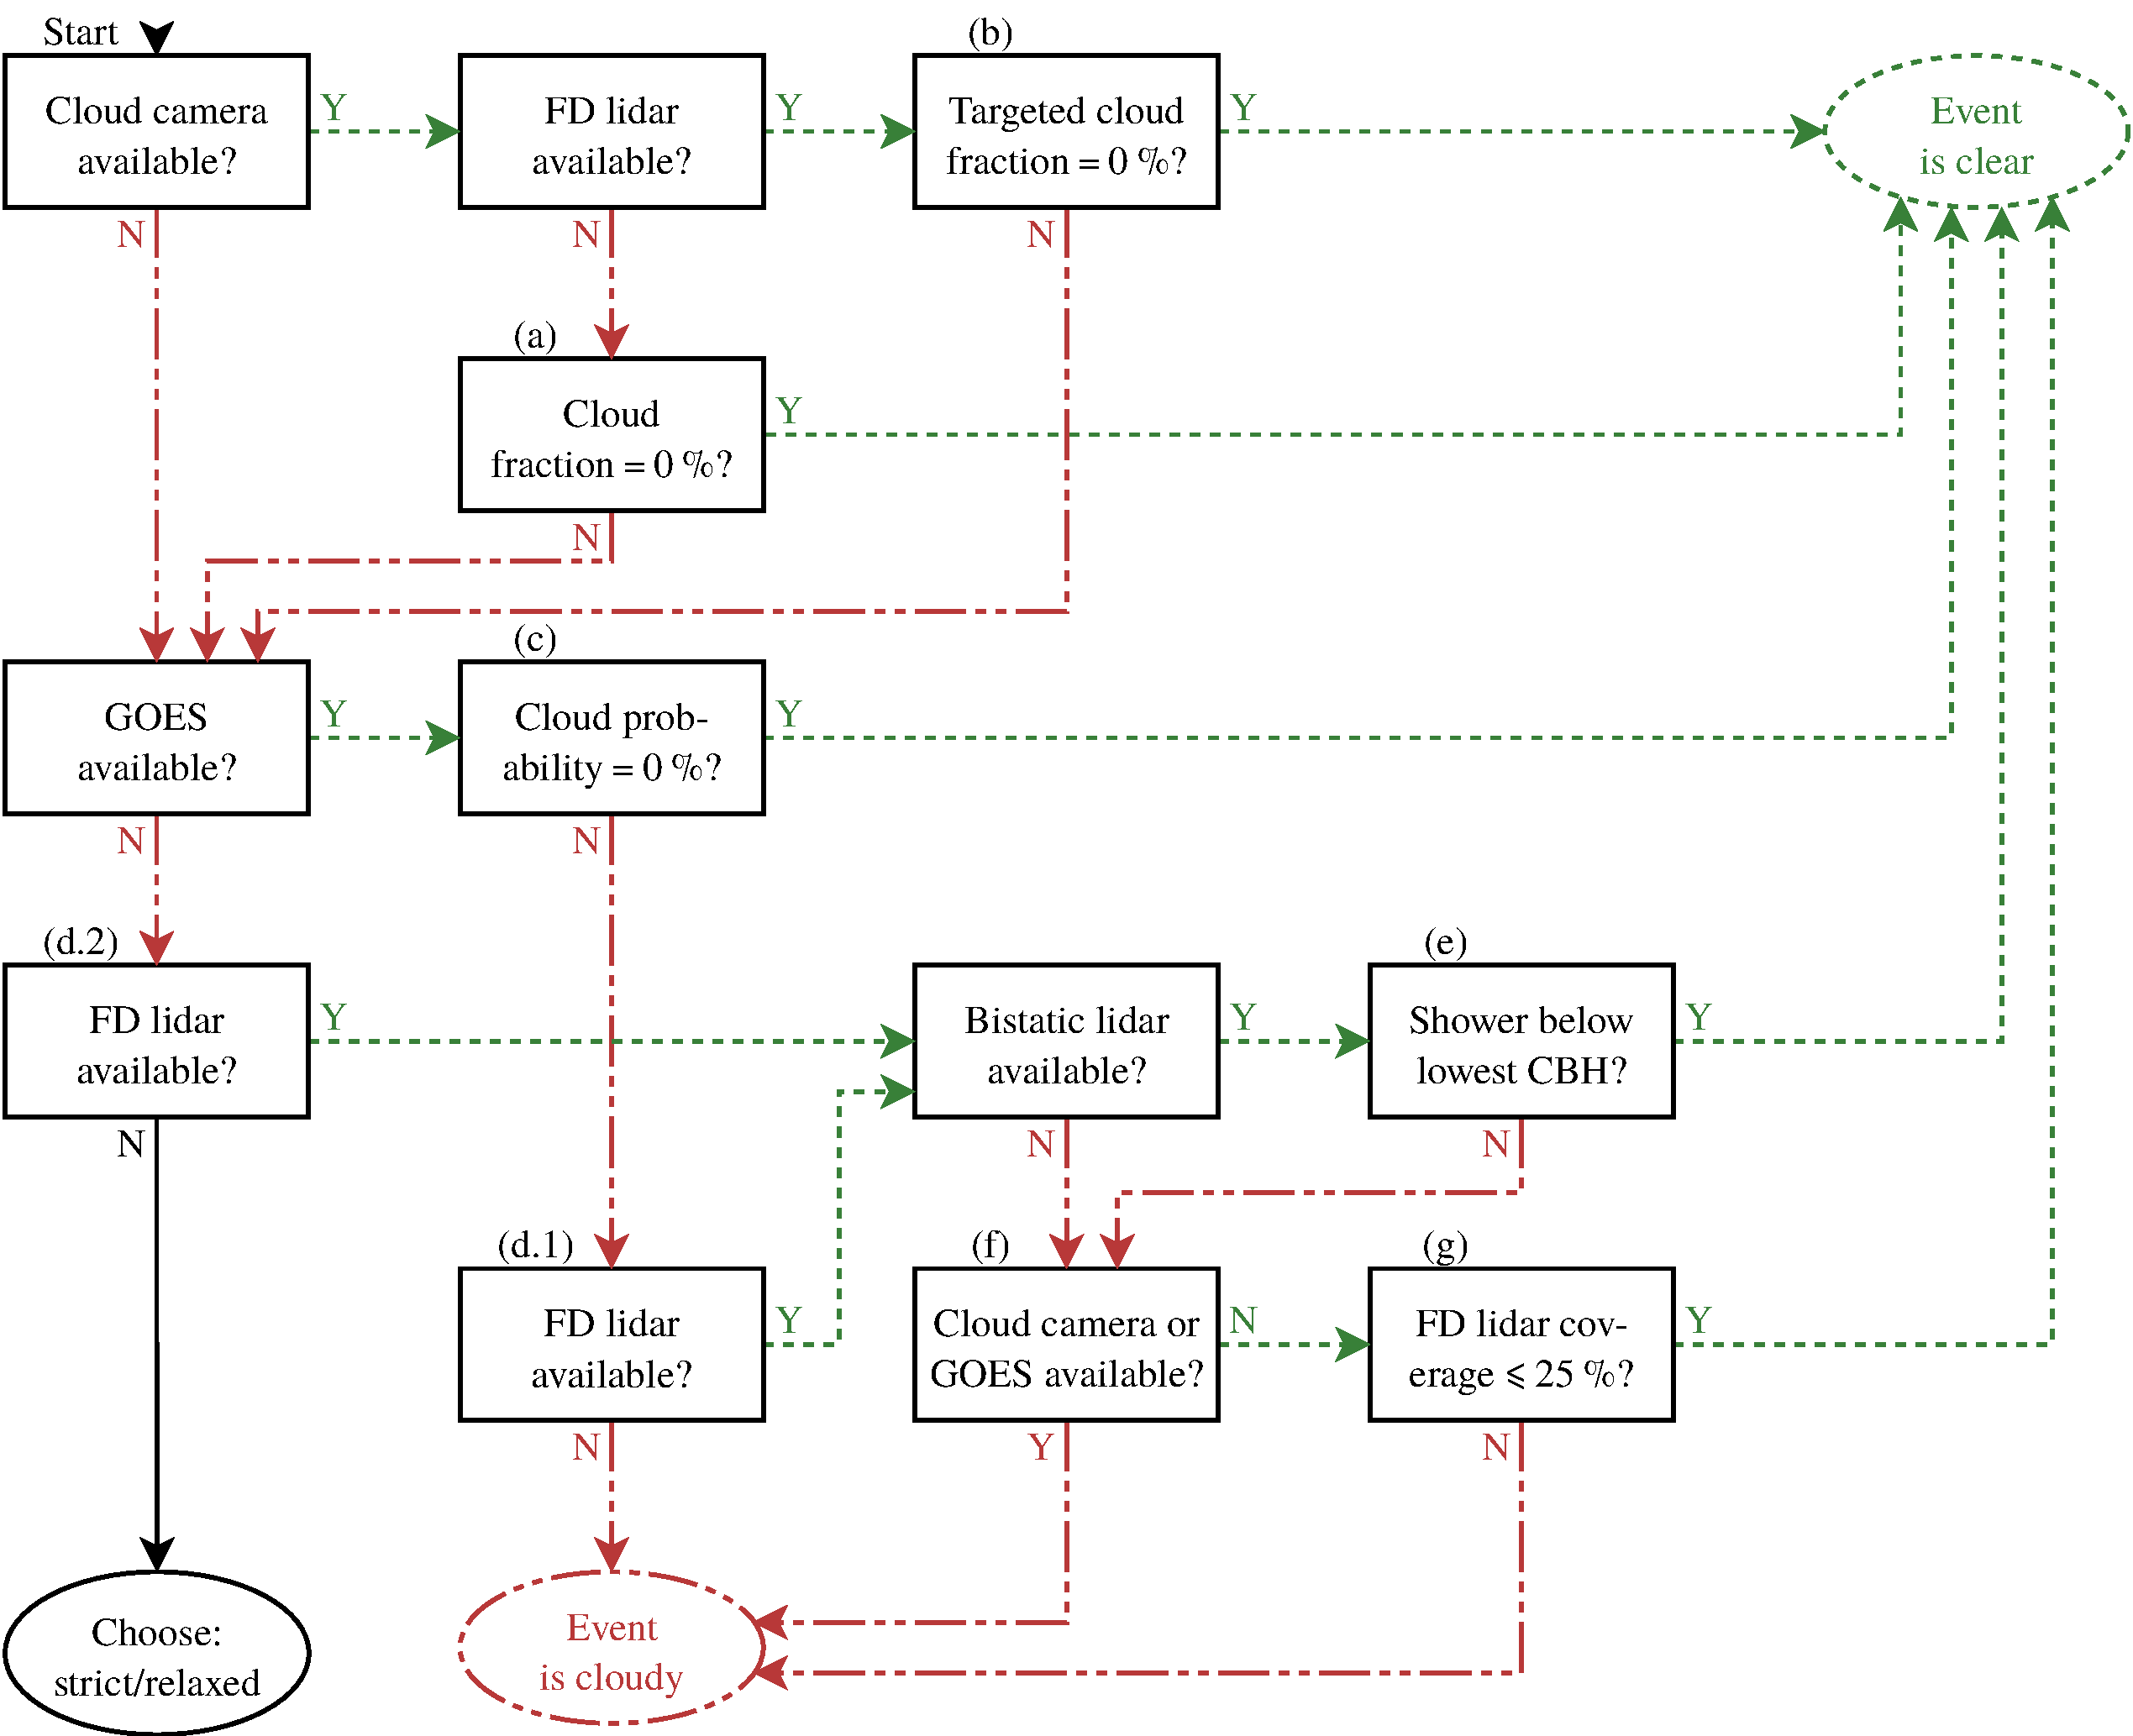
\includegraphics[width=0.7\textwidth]{chapters/graphs/CloudFlags/cloud_cuts.pdf}
\caption{Diagram of how the cloud cuts are applied to the data set when called with the Auger event selection program. Image provide by permission from V. Harvey} \label{fig:Cloud_Cut_Logic}
\end{figure}

Atmospheric measurements from the instruments described in Section \ref{sec:MonitoringEquipment} are processed and cloud probabilities are calculated. This data is then used within the Cloud cut to flag whether an event should be accepted or rejected. Within the Cloud cuts are checks to accommodate the multiple cloud data sources, both individually and in combination with each other. Figure \ref{fig:Cloud_Cut_Logic} shows the logic currently employed within the Cloud cut. The first check starts at (a) as go through to (f).  If an event passes a cut no further checks are performed.

\begin{itemize}
\item[(a)] If IR Cloud Mask is available for the pixels involved, an event will pass if there is 0\% cloud fraction. The cloud fraction is not calculated for pixel below 5.5\textdegree \ elevation. 
\item[(b)] Similar to step (a) but combines the nearest available FD lidar to determine the CBH to help whether the cloud is in front or behind the shower. The cloud mask fraction for pixels can be ignored if the CBH shows that the observed shower is below the cloud. Each pixel cloud fraction is recalculated and the event will pass if the total cloud fraction along the shower path is 0\%.
\item[(c)] If GOES data is available, this data is used to calculate the cloud probability between the FD site and the observed shower axis. If the cloud probability along the shower path is 0\% then the event will pass.
\item[(d)] No further steps are attempted if no FD lidar is available.
\begin{itemize}
\item[(d.1)] If all the above information is available and the event does not pass any of the cuts the event is flagged as being cloud effected.
\item[(d.2)] If none of the above information is available then the event cannot be flagged as either unaffected by could or not. The event is retained or discarded whether a "strict" or "relaxed" flag is set in the cloud cut settings. The relaxed setting is generally used but this is dependent on the analysis performed.
\end{itemize}
\item[(e)] If FD lidar and bistatic lidar data is available and no cloud camera or GOES information is available. The FD lidar and bistatics lidar can be used to determine the CBH. If the shower is below the lowest value of measured CBH the event will pass.
\item[(f)] If the event fails the condition in (e) or no data from the bistatic laser is available the event is checked to see if it has been flagged as cloudy by either the cloud camera or GOES data. If neither the cloud camera or GOES data is available then one last check is performed.
\item[(g)] The FD lidar data is used to determine the cloud coverage above the FD FoV. If the cloud coverage is less than 25\% the event is flagged as clear.
\end{itemize}



\section{Cloud Flags Investigation Method}

%Take reconstructed Golden Hybrid events from 2004 to 2018 
%
%Extract camera flag data.
%
%Two set of camera flags - positive ones that say that an event has pass one of the conditions saying that these is no cloud. the negative flags say that the event has failed to pass any of the test looking for clouds. If the flag is zero then there is no cloud information available.
%
%Four different flags - IR Cloud camera, LIDAR, GOES satellite data and something else.
%
%Look at the histograms of Xmax distributions for data passing cloud cuts, data failing cloud cuts and combined.

\begin{table}
\centering
\begin{tabular}{|c c|}
\hline 
\multicolumn{2}{|c|}{\textbf{==== reject laser events ====}} \\ \hline
!isCLF & \\
!isXLF & \\
\hline
\multicolumn{2}{|c|}{\textbf{==== keep either CO/HEAT or HECO ====}} \\ \hline
keepHECOorCoihuecoHEAT & 18.1 { nMinusOne: 21  -10.5 10.5 } \\
eyeCut & 1111 \\
\hline
\multicolumn{2}{|c|}{\textbf{==== hardware status ====}} \\ \hline
badFDPeriodRejection & \\
minMeanPixelRMSMergedEyes & {  params: 17 6 110000 nMinusOne: 100  0 100 } \\
minMeanPixelRMSSimpleEyes & {  params: 17 11111 nMinusOne: 100  0 100 } \\
!badPixels  &               1 \\
good10MHzCorrection & \\
\hline
\multicolumn{2}{|c|}{\textbf{==== atmosphere ====}} \\ \hline
hasMieDatabase & \\
maxVAOD & 0.1 \\
cloudCutXmaxPRD14  & { params: 1 nMinusOne: 21  -10.5 10.5 } \\
\hline
\multicolumn{2}{|c|}{\textbf{==== full hybrid geometry ====}} \\ \hline
hybridTankTrigger &       2 \\
maxCoreTankDist & 1500 \\
maxZenithFD       &        90 \\
minLgEnergyFD    &        1e-20 \\
skipSaturated & \\
minPBrass         &        0.9 \\
maxPBrassProtonIronDiff &  0.05 \\
minLgEnergyFD     &       17.8 \\
\hline
\multicolumn{2}{|c|}{\textbf{==== FOV cuts ====}} \\ \hline
FidFOVICRC13 & 40 20 \\
\hline
\multicolumn{2}{|c|}{\textbf{==== quality cuts ====}} \\ \hline
xMaxObsInExpectedFOV & { params: 40 20 } \\
maxDepthHole    &     20. \\
profileChi2Sigma  &  {  params:  3 -1.1 nMinusOne: 400  -20 20 } \\
depthTrackLength   &  200 \\ \hline
\end{tabular}
\caption{Relaxed cloud cut version of PRD14 cut} \label{tab:Quality_Cuts}
\end{table}


The method used to investigate the effects of the cloud cuts on the Auger data was applied to the Golden Hybrid data set with events from 2004 to 2018. First the events where reconstructed through the Auger OffLine program and then the reconstructed events where passed through a selectEvents program. This selectEvents program utilises a series of parameters to apply quality cuts to the reconstructed events. The list of cuts used are shown in Tab \ref{tab:Quality_Cuts}. The cuts used on the data set for the ICRC2019 list of cuts is taken from within the collaboration OffLine application. Once a standard set of events was produced, another set was produced where all of the cuts were applied except for the Cloud Cuts. 

After these two data sets where produced, I then took the code that would assign the cloud flag to an event and then used it within my own analysis code. The code was then used to apply a flag number to indicate which of the cloud cuts the event would pass or fail. I assigned a positive value between 1 and 5 to say that the event was cloud free. The number indicates which monitoring instrument said that there was no clouds between the event and the triggered Fluorescence Telescope (FD). A zero meant that there was no data from any monitoring instrument. A negative number was used to denote that the cloud data from the monitoring instrument indicated that the threshold was triggered to say that the event should be rejected. 

From there I looked into the Elongation Rate (Xmax vs log$_{10}$(Energy)) which is of concern for any study involving mass composition. I will show the distributions of events in log$_{10}$(Energy) and Xmax. The Xmax plots are split up into different energy bins to see the distributions. I was particularly interested in quantifying the tails of these distributions as they would be of most concern to the mass composition studies. Any mass composition analysis needs to have confidence in the calculation of the mean and standard deviation which is used to indicate the average composition of events within a particular energy bin. Removing or adding a quality cut is done with a lot of considerations in mind. Outside of mass composition, there will be other studies that are not as concerned with tails of the Xmax distributions.

I also show examples of individual events that would and would not pass the cloud cuts. This is to give a visual indication of what events that would pass look like and compare this to events that would fail the cloud cut. I have also shown some events that have weird properties which I will explain further within the results and discussion section.


\section{Results - Effect on Mean Xmax and Spread in Xmax}

%- Cloud Cut Flags distribution
%
%- Xmax distributions within energy bins
%
%- Elongation rate  
%
%- Is distance to Xmax or distance to shower axis needed?

\subsection{Cloud Flags Distribution}

Figure \ref{fig:cloudFlag_dist} shows the distribution of reconstruction shower events that would pass all quality cuts what Cloud Cut Flag has been assigned to them. Greater than zero means that the event has passed one of the cases to say that the event has a high probability it has not been effected by clouds. Less than zero means that the event has had a cloud detected close enough in space or time with a high probability to have had an effect. Minus one denotes events that have failed the cloud camera and/or the lidar condition, minus two denotes events that have failed the GOES data condition and minus three are events that have failed combinations of CLF/XLF, GOES data, Cloud camera and lidar conditions. Zero means that there is no definite measurement that the event has or has not been effected by clouds. Events with the zero flag are kept or discarded whether the relaxed or strict settings are used. In this case the relaxed setting was used so the events with flag equal to zero were marked as considered to not having any cloud.

\subsection{Elongation Rate}


\begin{figure}[!hp]
\centering
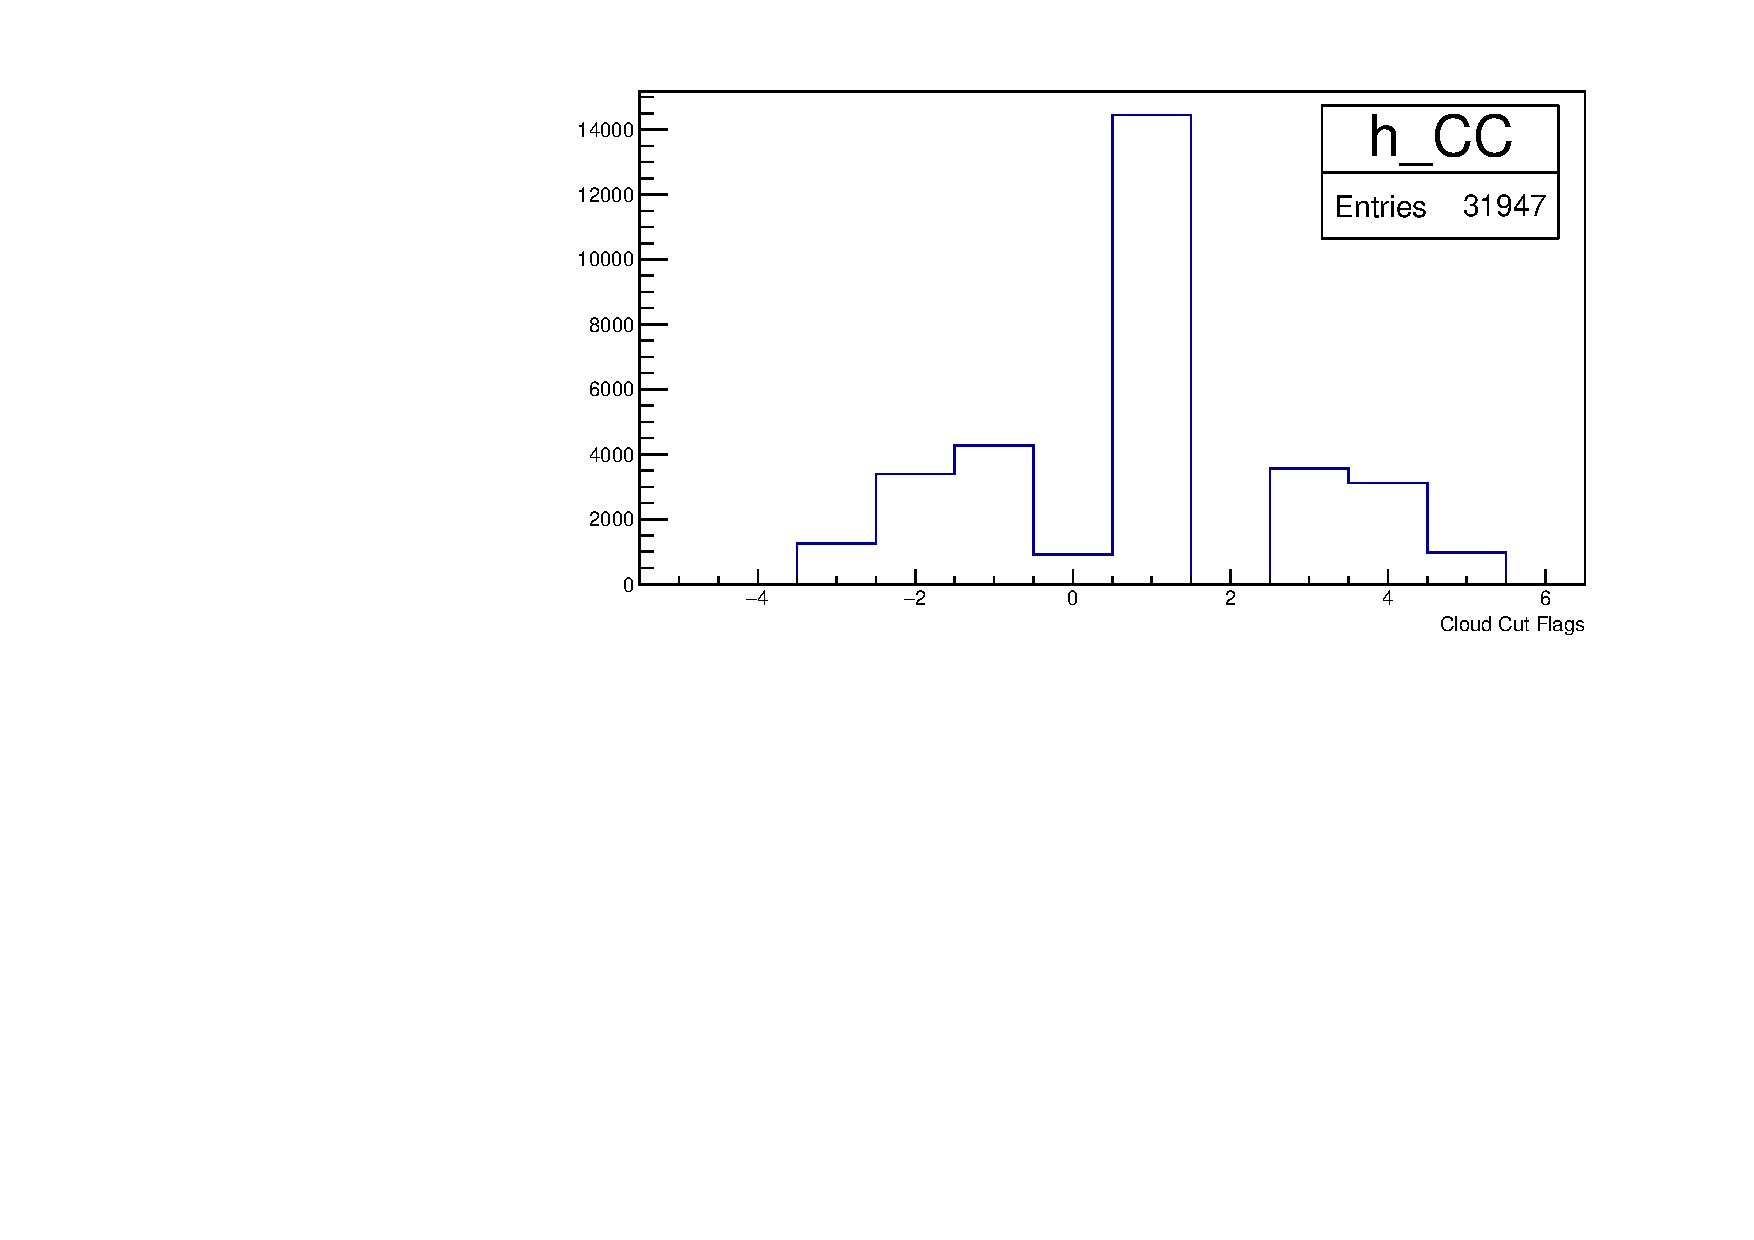
\includegraphics[width=\textwidth]{chapters/graphs/CloudFlags/hist_cloudFlags.pdf}
\caption{Distribution of cloud flags. Positive flag values are for events that would pass one of the cloud cuts. Negative flag values are for events that would fail one of the cloud cuts. A flag value of zero is for events that have no cloud data.}\label{fig:cloudFlag_dist}
\end{figure}

\begin{figure}[!hp]
\centering
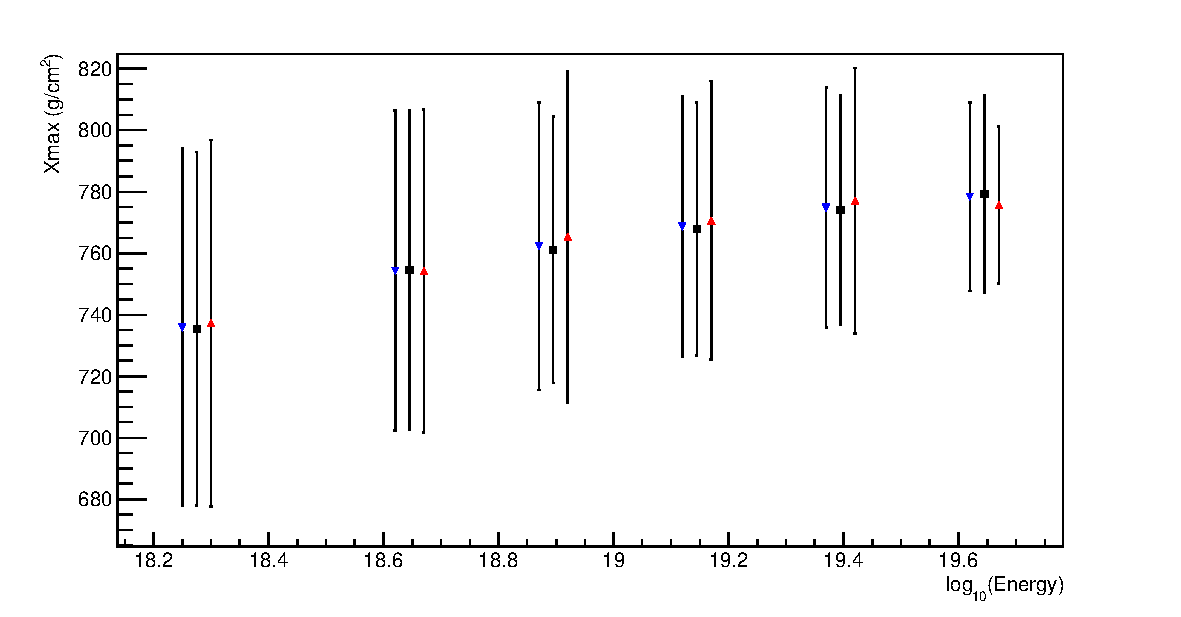
\includegraphics[width=\textwidth]{chapters/graphs/CloudFlags/ElongationRate.pdf}
\caption{Elongation Rate with Cloud cuts applied (blue downward triangle), without any cloud cuts (black square) and only events that would fail the cloud cuts (red upward triangle). The uncertainity bars denote the standard deviation of each distribution.} \label{fig:ElongRate_hist}
\end{figure}

Figure \ref{fig:ElongRate_hist} shows how the elongation rate as a function of energy. This figure shows the mean and standard deviation of Xmax within each energy bin. The standard deviation is shown as it is of importance to mass composition studies. There is no significance difference between the elongation  rates of the different data sets with Cloud Cuts applied (blue downwards triangles), without any Cloud Cuts (black squares) and only events that would fail the cloud cuts (red upward triangles).

% Energy Distribution

\subsection{Spectrum of events by Energy}

Comparison distributions of the energy spectrum observed by Auger were made. The events are selected, after being successfully reconstructed, by passing through a series of quality cuts. The comparison was done on data sets that contain events that only pass the cloud cut, only fail the cloud cut and a data set with the cloud cut is removed. Figure \ref{fig:cloudFlag_energyDist} shows the number events per energy bin above 10$^{18}$ eV. The distribution shows how the shape of the distribution is not affected by whether clouds are present or not. This is a good sign as clouds should not preferentially block events at any particular energy. The only difference is the total number of events in each energy bin.

\begin{figure}[!t]
\centering
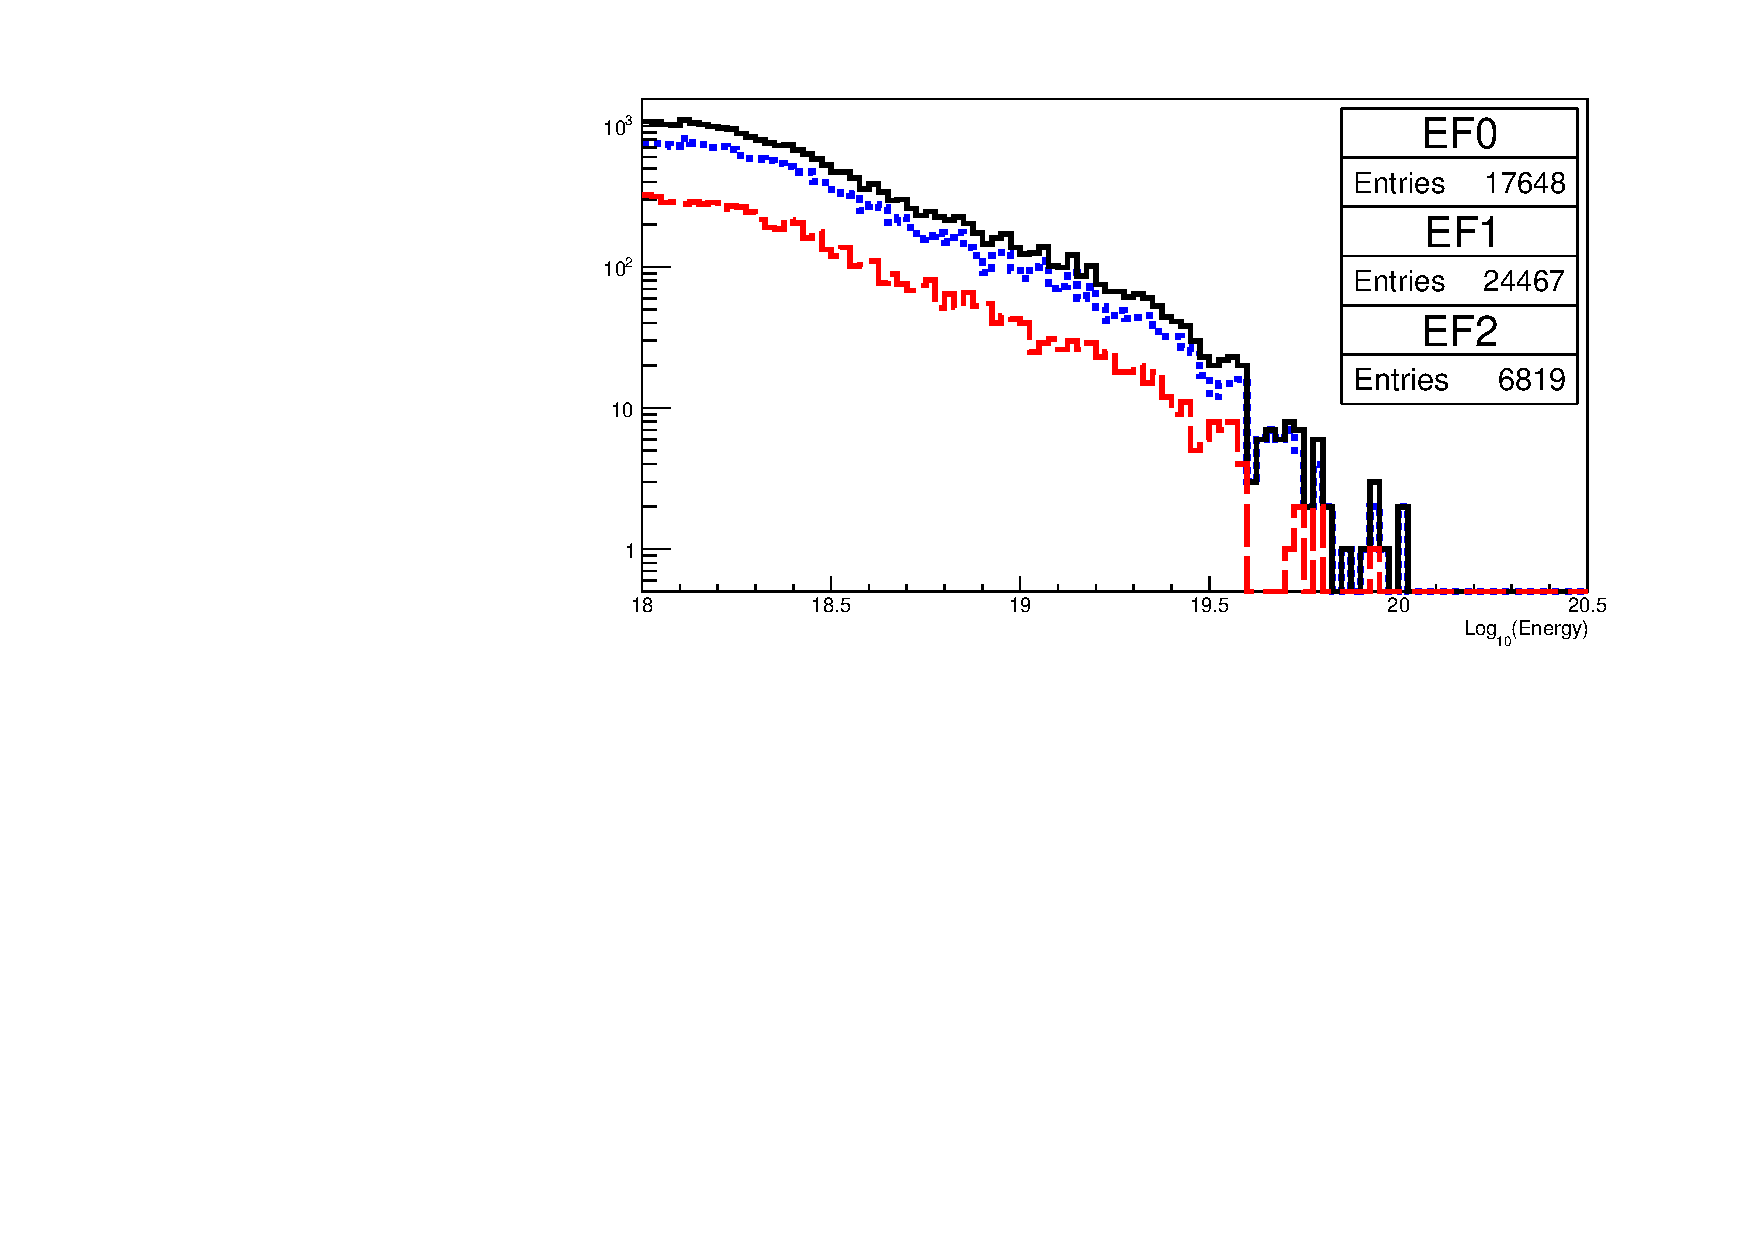
\includegraphics[width=\textwidth]{/home/tsudholz/PhD/Thesis/chapters/graphs/CloudFlags/EnergyHistAll_logE_18_0to20_5_Comb2.pdf}
\caption{Distribution of the energy of events within the bin of log(E) of 18.0 to 20.5. Black (EF1) denotes events that passed with the cloud cut removed, blue (EF0) denotes events that would pass the cloud cuts and red (EF2) denotes events that would fail the cloud cuts. All other cuts used for the ICRC19 have been applied.} \label{fig:cloudFlag_energyDist}
\end{figure}

%\begin{figure}
%\centering
%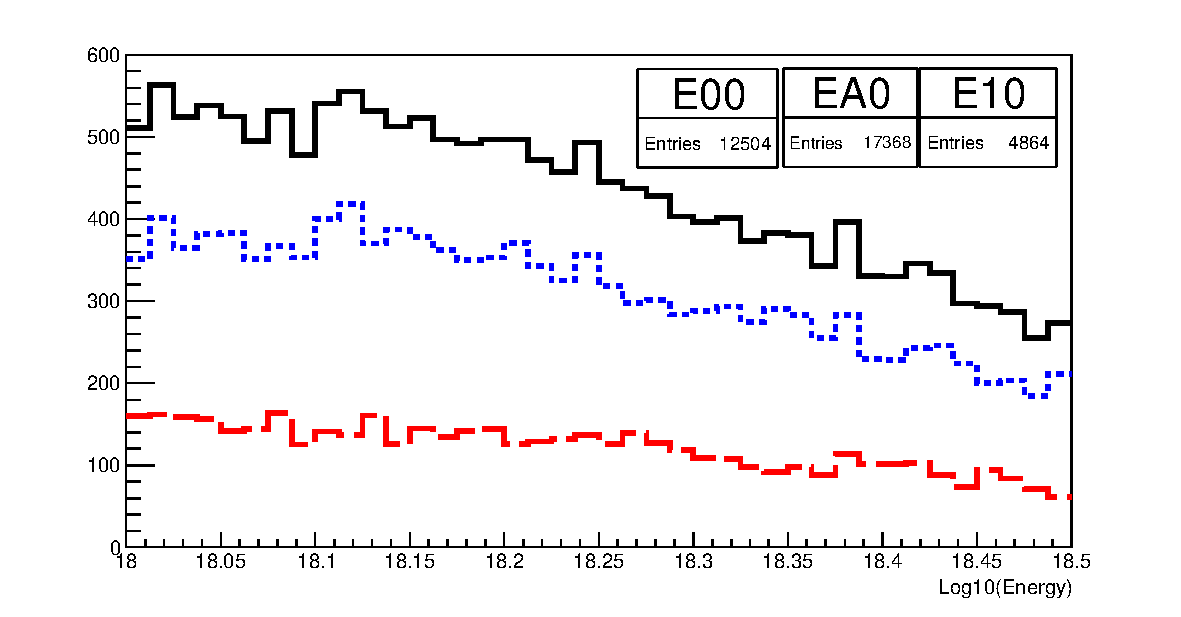
\includegraphics[width=\textwidth]{/home/tsudholz/PhD/Thesis/chapters/graphs/CloudFlags/EnergyHist_logE_18_0to18_5_Comb.pdf}
%\caption{Distribution of the energy of events within the bin of log(E) of 18.0 to 18.5. Black (EA0) denotes events that passed with cloud cut removed, blue (E00) denotes events that would pass the cloud cuts and red (E10) denotes events that would fail the cloud cuts. All other cuts used for the ICRC19 have been applied.}
%\end{figure}
%
%\begin{figure}
%\centering
%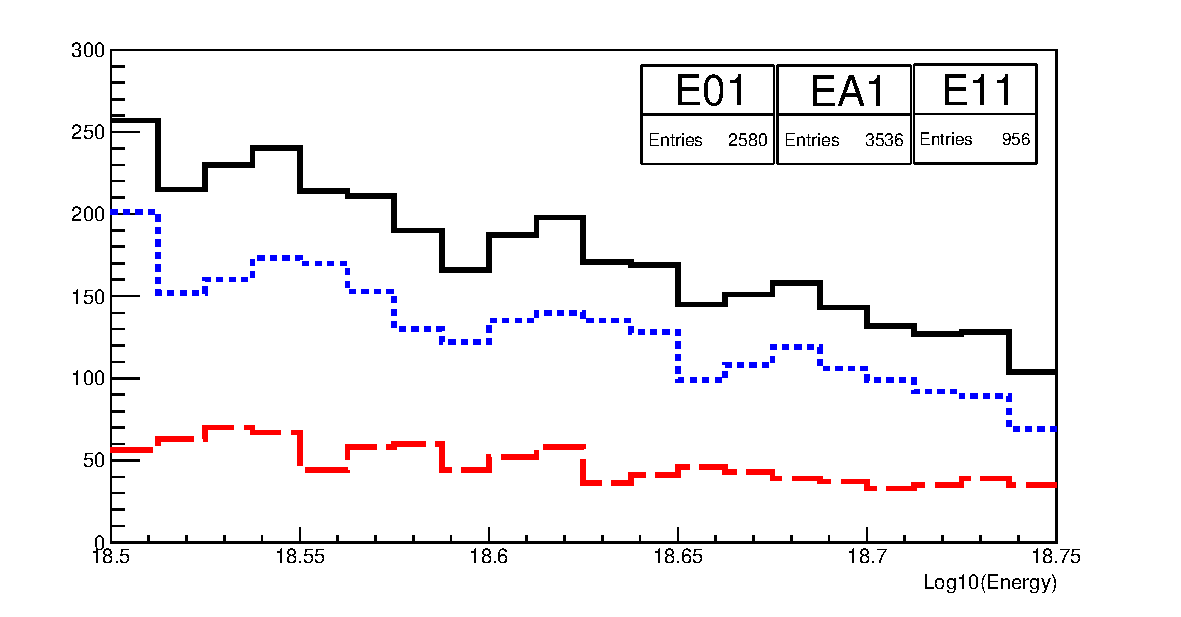
\includegraphics[width=\textwidth]{/home/tsudholz/PhD/Thesis/chapters/graphs/CloudFlags/EnergyHist_logE_18_5to18_75_Comb.pdf}
%\caption{Distribution of the energy of events within the bin of log(E) of 18.5 to 18.75. Black (EA1) denotes events that passed with cloud cut removed, blue (E01) denotes events that would pass the cloud cuts and red (E11) denotes events that would fail the cloud cuts. All other cuts used for the ICRC19 have been applied. }
%\end{figure}
%
%\begin{figure}
%\centering
%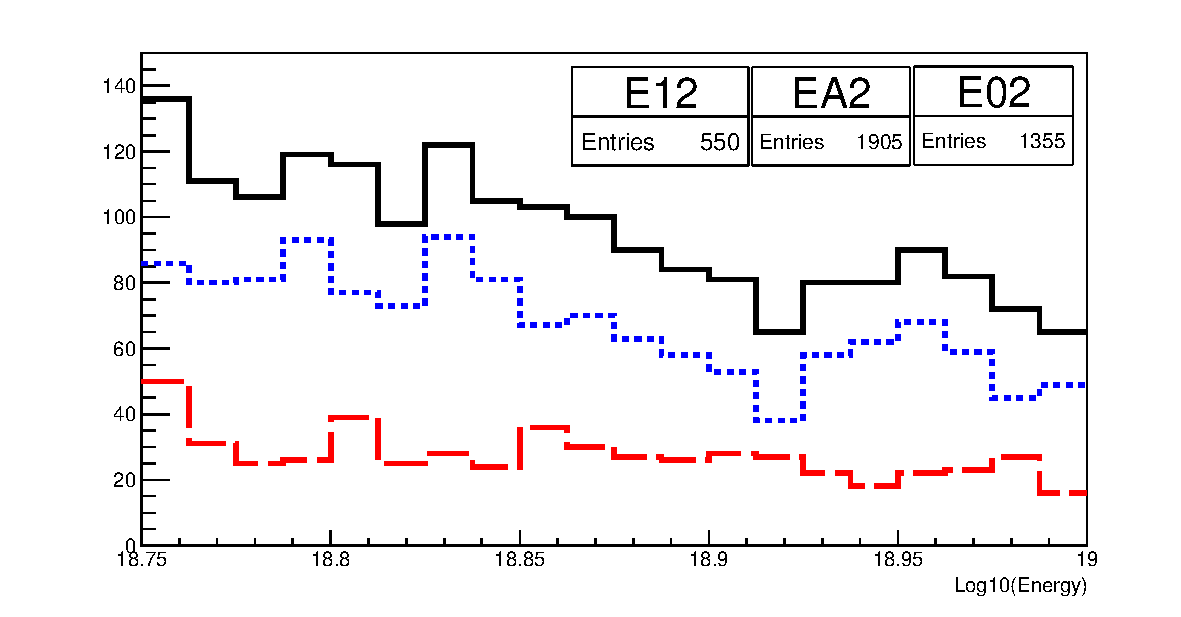
\includegraphics[width=\textwidth]{/home/tsudholz/PhD/Thesis/chapters/graphs/CloudFlags/EnergyHist_logE_18_75to19_0_Comb.pdf}
%\caption{Distribution of the energy of events within the bin of log(E) of 18.75 to 19.0. Black (EA2) denotes events that passed with cloud cut removed, blue (E12) denotes events that would pass the cloud cuts and red (E02) denotes events that would fail the cloud cuts. All other cuts used for the ICRC19 have been applied.}
%\end{figure}
%
%\begin{figure}
%\centering
%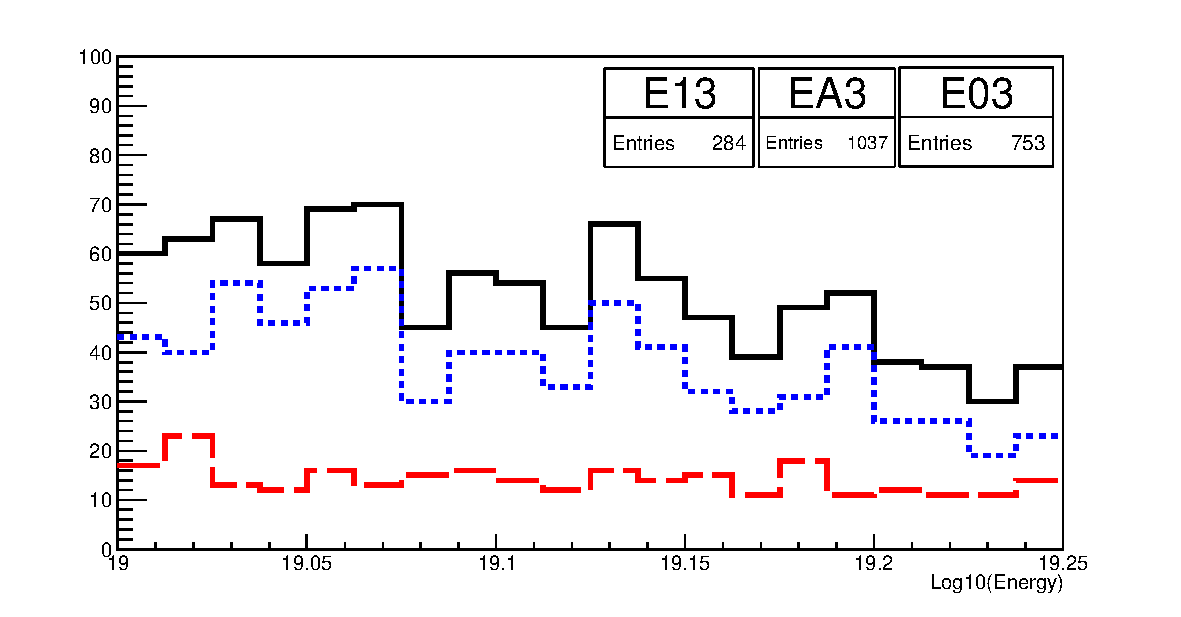
\includegraphics[width=\textwidth]{/home/tsudholz/PhD/Thesis/chapters/graphs/CloudFlags/EnergyHist_logE_19_0to19_25_Comb.pdf}
%\caption{Distribution of the energy of events within the bin of log(E) of 19.0 to 19.25. Black (EA3) denotes events that passed with cloud cut removed, blue (E13) denotes events that would pass the cloud cuts and red (E03) denotes events that would fail the cloud cuts. All other cuts used for the ICRC19 have been applied.}
%\end{figure}
%
%\begin{figure}
%\centering
%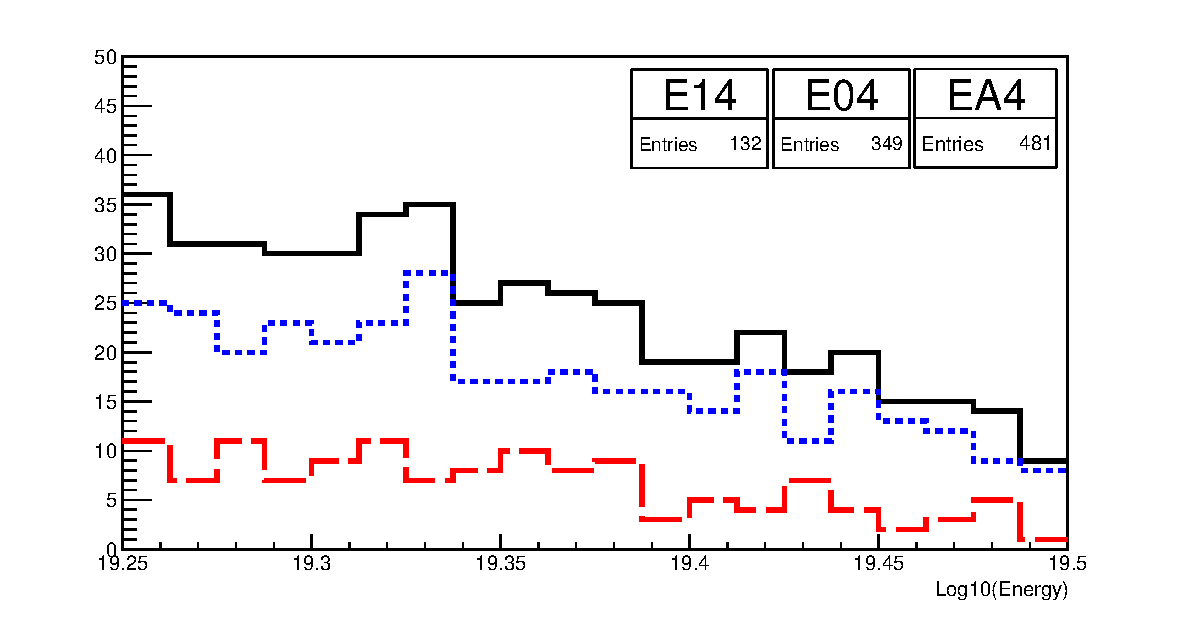
\includegraphics[width=\textwidth]{/home/tsudholz/PhD/Thesis/chapters/graphs/CloudFlags/EnergyHist_logE_19_25to19_5_Comb.pdf}
%\caption{Distribution of the energy of events within the bin of log(E) of 19.25 to 19.5. Black (EA4) denotes events that passed with cloud cut removed, blue (E14) denotes events that would pass the cloud cuts and red (E04) denotes events that would fail the cloud cuts. All other cuts used for the ICRC19 have been applied.}
%\end{figure}
%
%\begin{figure}
%\centering
%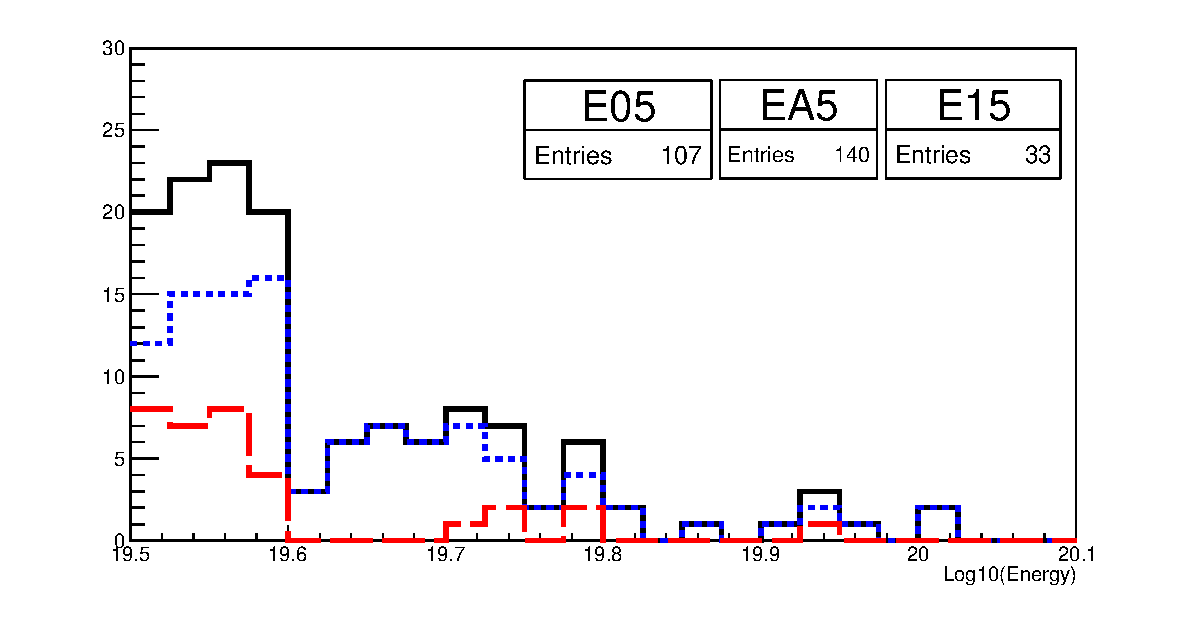
\includegraphics[width=\textwidth]{/home/tsudholz/PhD/Thesis/chapters/graphs/CloudFlags/EnergyHist_logE_Greater19_5_Comb.pdf}
%\caption{Distribution of the energy of events within the bin of log(E) of greater than 19.5. Black (EA5) denotes events that passed with cloud cut removed, blue (E15) denotes events that would pass the cloud cuts and red (E05) denotes events that would fail the cloud cuts. All other cuts used for the ICRC19 have been applied.}
%\end{figure}

% Xmax Distribution for Passed, Combined, Failed

\subsection{Xmax Distribution}




\begin{figure}[!p]
\centering
\includegraphics[width=\textwidth]{/home/tsudholz/PhD/Thesis/chapters/graphs/CloudFlags/NormHist_Xmax_logE_18_0to18_5_Comb.pdf}
\caption{Distribution of the Xmax of events within the bin of log(E) of 18.0 to 18.5. Black (XA0) denotes events that passed with cloud cut removed, blue (X00) denotes events that would pass the cloud cuts and red (X10) denotes events that would fail the cloud cuts. All other cuts used for the ICRC19 have been applied.} \label{fig:CloudFlag_XmaxDist_18.0}
\end{figure}

\begin{figure}[!p]
\centering
\includegraphics[width=\textwidth]{/home/tsudholz/PhD/Thesis/chapters/graphs/CloudFlags/NormHist_Xmax_logE_18_5to18_75_Comb.pdf}
\caption{Distribution of the Xmax of events within the bin of log(E) of 18.5 to 18.75. Black (XA1) denotes events that passed with cloud cut removed, blue (X01) denotes events that would pass the cloud cuts and red (X11) denotes events that would fail the cloud cuts. All other cuts used for the ICRC19 have been applied.}\label{fig:CloudFlag_XmaxDist_18.5}
\end{figure}

\begin{figure}[!p]
\centering
\includegraphics[width=\textwidth]{/home/tsudholz/PhD/Thesis/chapters/graphs/CloudFlags/NormHist_Xmax_logE_18_75to19_0_Comb.pdf}
\caption{Distribution of the Xmax of events within the bin of log(E) of 19.0 to 19.25. Black (XA2) denotes events that passed with cloud cut removed, blue (X02) denotes events that would pass the cloud cuts and red (X12) denotes events that would fail the cloud cuts. All other cuts used for the ICRC19 have been applied.}\label{fig:CloudFlag_XmaxDist_18.75}
\end{figure}

\begin{figure}[!p]
\centering
\includegraphics[width=\textwidth]{/home/tsudholz/PhD/Thesis/chapters/graphs/CloudFlags/NormHist_Xmax_logE_19_0to19_25_Comb.pdf}
\caption{Distribution of the Xmax of events within the bin of log(E) of 19.0 to 19.25. Black (XA3) denotes events that passed with cloud cut removed, blue (X03) denotes events that would pass the cloud cuts and red (X13) denotes events that would fail the cloud cuts. All other cuts used for the ICRC19 have been applied.}\label{fig:CloudFlag_XmaxDist_19.0}
\end{figure}

\begin{figure}[!p]
\centering
\includegraphics[width=\textwidth]{/home/tsudholz/PhD/Thesis/chapters/graphs/CloudFlags/NormHist_Xmax_logE_19_25to19_5_Comb.pdf}
\caption{Distribution of the Xmax of events within the bin of log(E) of 19.25 to 19.5. Black (XA4) denotes events that passed with cloud cut removed, blue (X04) denotes events that would pass the cloud cuts and red (X14) denotes events that would fail the cloud cuts. All other cuts used for the ICRC19 have been applied.}\label{fig:CloudFlag_XmaxDist_19.25}
\end{figure}

\begin{figure}[!p]
\centering
\includegraphics[width=\textwidth]{/home/tsudholz/PhD/Thesis/chapters/graphs/CloudFlags/NormHist_Xmax_logE_Greater19_5_Comb.pdf}
\caption{Distribution of the Xmax of events within the bin of log(E) of greater than 19.5. Black (XA5) denotes events that passed with cloud cut removed, blue (X05) denotes events that would pass the cloud cuts and red (X15) denotes events that would fail the cloud cuts. All other cuts used for the ICRC19 have been applied.}\label{fig:CloudFlag_XmaxDist_19.5}
\end{figure}

Comparison of Xmax distributions between data sets with the cloud cut, without the cloud cut and a data set that just contains events that would fail the cloud cut. Each of these distributions has been normalised as each distribution has different amounts and it allows the shape to be more easily compared. The dataset is split into six log$_{10}$(energy) bins to show the Xmax distribution: 18.0 to 18.5, 18.5 to 18.75, 18.75 to 19.0, 19.0 to 19.25, 19.25 to 19.5 and greater than 19.5. From looking at the mean and standard deviations each of the distributions are not significantly different. From Figure \ref{fig:CloudFlag_XmaxDist_18.0} to Figure \ref{fig:CloudFlag_XmaxDist_19.5} the black continuous line denotes all events that pass just the quality cuts with the cloud cuts removed, blurs points denote the events that would pass all the quality cuts including the cloud cuts and red denotes events that would pass all the quality cuts except for the cloud cuts.

Adding the rejected events back into the distribution allows the number of events to increase by around 30\%. This is a great addition to the highest energy bin (in this case $>$ 10$^{19.5}$ eV) where the statistics are low.

% Xmax Distribution for Failed only

\subsection{Xmax Distribution for Events that Failed Cloud Cut}



\begin{figure}[!p]
\centering
\includegraphics[width=\textwidth]{/home/tsudholz/PhD/Thesis/chapters/graphs/CloudFlags/NormHist_Xmax_FailedCloudCut_logE_18_0to18_5_Comb.pdf}
\caption{Distribution of the energy of events within the bin of log(E) of 18.0 to 18.5. Red (X10) denotes all event that failed the cloud cuts, black (X20) denotes events that failed the cloud camera/lidar cut, blue (X30) denotes events that failed the GOES data cut and green (X40) are events that have fail a combination of CLF/XLF, GOES and Cloud camera cut.} \label{fig:CloudFlag_XmaxFailed_18.0}
\end{figure}

\begin{figure}[!p]
\centering
\includegraphics[width=\textwidth]{/home/tsudholz/PhD/Thesis/chapters/graphs/CloudFlags/NormHist_Xmax_FailedCloudCut_logE_18_5to18_75_Comb.pdf}
\caption{Distribution of the energy of events within the bin of log(E) of 18.5 to 18.75. Red (X11) denotes all event that failed the cloud cuts, black (X21) denotes events that failed the cloud camera/lidar cut, blue (X31) denotes events that failed the GOES data cut and green (X41) are events that have fail a combination of CLF/XLF, GOES and Cloud camera cut.} \label{fig:CloudFlag_XmaxFailed_18.5}
\end{figure}

\begin{figure}[!p]
\centering
\includegraphics[width=\textwidth]{/home/tsudholz/PhD/Thesis/chapters/graphs/CloudFlags/NormHist_Xmax_FailedCloudCut_logE_18_75to19_0_Comb.pdf}
\caption{Distribution of the energy of events within the bin of log(E) of 18.75 to 19.0. Red (X12) denotes all event that failed the cloud cuts, black (X22) denotes events that failed the cloud camera/lidar cut, blue (X32) denotes events that failed the GOES data cut and green (X42) are events that have fail a combination of CLF/XLF, GOES and Cloud camera cut.} \label{fig:CloudFlag_XmaxFailed_18.75}
\end{figure}

\begin{figure}[!p]
\centering
\includegraphics[width=\textwidth]{/home/tsudholz/PhD/Thesis/chapters/graphs/CloudFlags/NormHist_Xmax_FailedCloudCut_logE_19_0to19_25_Comb.pdf}
\caption{Distribution of the energy of events within the bin of log(E) of 19.0 to 19.25. Red (X13) denotes all event that failed the cloud cuts, black (X23) denotes events that failed the cloud camera/lidar cut, blue (X33) denotes events that failed the GOES data cut and green (X43) are events that have fail a combination of CLF/XLF, GOES and Cloud camera cut.} \label{fig:CloudFlag_XmaxFailed_19.0}
\end{figure}

\begin{figure}[!p]
\centering
\includegraphics[width=\textwidth]{/home/tsudholz/PhD/Thesis/chapters/graphs/CloudFlags/NormHist_Xmax_FailedCloudCut_logE_19_25to19_5_Comb.pdf}
\caption{Distribution of the energy of events within the bin of log(E) of 19.25 to 19.5. Red (X14) denotes all event that failed the cloud cuts, black (X24) denotes events that failed the cloud camera/lidar cut, blue (X34) denotes events that failed the GOES data cut and green (X44) are events that have fail a combination of CLF/XLF, GOES and Cloud camera cut.} \label{fig:CloudFlag_XmaxFailed_19.25}
\end{figure}

\begin{figure}[!p]
\centering
\includegraphics[width=\textwidth]{/home/tsudholz/PhD/Thesis/chapters/graphs/CloudFlags/NormHist_Xmax_FailedCloudCut_logE_Greater19_5_Comb.pdf}
\caption{Distribution of the energy of events within the bin of log(E) of greater than 19.5. Red (X15) denotes all event that failed the cloud cuts, black (X25) denotes events that failed the cloud camera/lidar cut, blue (X35) denotes events that failed the GOES data cut and green (X45) are events that have fail a combination of CLF/XLF, GOES and Cloud camera cut.} \label{fig:CloudFlag_XmaxFailed_19.5}
\end{figure}

Figures \ref{fig:CloudFlag_XmaxFailed_18.0} to Figure \ref{fig:CloudFlag_XmaxFailed_19.5} show the distributions of events that failed the cloud cuts split into 3 different flag types. Red denotes all event that failed the cloud cuts, black denotes events that failed the cloud camera/lidar cut, blue denotes events that failed the GOES data cut and green are events that have fail a combination of CLF/XLF, GOES and Cloud camera cut. 

These distributions show that the majority of events are rejected by the cloud camera/lidar cut or by the GOES satellite cut. A smaller faction of events are rejected by a combination of CLF/XLF, GOES and Cloud camera/lidar cut.

\subsection{Graphical Examples of Events from within the tails of the Xmax distributions}

% Events that would fail the cloud cut only

\begin{figure}[!p]
\centering
  \settoheight{\tempheight}{\includegraphics[width=0.45\textwidth , trim = 0 0 5.5cm 0]{/home/tsudholz/PhD/Thesis/chapters/graphs/CloudFlags/CloudCut_Events_Failed/Auger_52704749200_FdEventInfo.pdf}}
 \vspace{2cm}
  \begin{subfigure}[b]{\textwidth}
  \centering
  \includegraphics[width=\textwidth]{/home/tsudholz/PhD/Thesis/chapters/graphs/CloudFlags/CloudCut_Events_Failed/Auger_52704749200_SlantDepth.pdf}
  \caption{FD profile of the energy deposited as a function of atmospheric depth.}
  \end{subfigure}
 \vspace{0.5cm}
  \begin{subfigure}[b]{0.45\textwidth}
  	\centering
  	\includegraphics[width=\textwidth , height=\tempheight]{/home/tsudholz/PhD/Thesis/chapters/graphs/CloudFlags/CloudCut_Events_Failed/Auger_52704749200_FdProfile.pdf}
  	\caption{FD light profile}
  \end{subfigure}
  \begin{subfigure}[b]{0.45\textwidth}
  	\centering
  	\includegraphics[width=0.8\textwidth , height=\tempheight]{/home/tsudholz/PhD/Thesis/chapters/graphs/CloudFlags/CloudCut_Events_Failed/Auger_52704749200_SdProfile.pdf}
  	\caption{SD tank triggered profile}
  \end{subfigure}

  \begin{subfigure}[b]{0.45\textwidth}
  	\centering
	\includegraphics[height=\tempheight , trim = 0 0 5.5cm 0]{/home/tsudholz/PhD/Thesis/chapters/graphs/CloudFlags/CloudCut_Events_Failed/Auger_52704749200_FdEventInfo.pdf}
  	\caption{FD Event Info}
  \end{subfigure}
  \begin{subfigure}[b]{0.45\textwidth}
  	\centering
	\includegraphics[height=\tempheight]{/home/tsudholz/PhD/Thesis/chapters/graphs/CloudFlags/CloudCut_Events_Failed/Auger_52704749200_SdEventInfo.pdf}
  	\caption{SD Event Info}
  \end{subfigure}
  \caption{Example of an Auger event that would fail the cloud selection cut from EventBrowser}
\end{figure}

\begin{figure}[!p]
\centering
  \settoheight{\tempheight}{\includegraphics[width=0.45\textwidth , trim = 0 0 5.5cm 0]{/home/tsudholz/PhD/Thesis/chapters/graphs/CloudFlags/CloudCut_Events_Failed/Auger_70735278500_FdEventInfo.pdf}}
 \vspace{2cm}
  \begin{subfigure}[b]{\textwidth}
  \centering
  \includegraphics[width=\textwidth]{/home/tsudholz/PhD/Thesis/chapters/graphs/CloudFlags/CloudCut_Events_Failed/Auger_160416430001_SlantDepth.pdf}
  \caption{FD profile of the energy deposited as a function of atmospheric depth.}
  \end{subfigure}
 \vspace{0.5cm}
  \begin{subfigure}[b]{0.45\textwidth}
  	\centering
  	\includegraphics[width=\textwidth , height=\tempheight]{/home/tsudholz/PhD/Thesis/chapters/graphs/CloudFlags/CloudCut_Events_Failed/Auger_160416430001_FdProfile.pdf}
  	\caption{FD light profile}
  \end{subfigure}
  \begin{subfigure}[b]{0.45\textwidth}
  	\centering
  	\includegraphics[width=0.8\textwidth , height=\tempheight]{/home/tsudholz/PhD/Thesis/chapters/graphs/CloudFlags/CloudCut_Events_Failed/Auger_160416430001_SdProfile.pdf}
  	\caption{SD tank triggered profile}
  \end{subfigure}

  \begin{subfigure}[b]{0.45\textwidth}
  	\centering
	\includegraphics[height=\tempheight , trim = 0 0 5.5cm 0]{/home/tsudholz/PhD/Thesis/chapters/graphs/CloudFlags/CloudCut_Events_Failed/Auger_160416430001_FdEventInfo.pdf}
  	\caption{FD light profile}
  \end{subfigure}
  \begin{subfigure}[b]{0.45\textwidth}
  	\centering
	\includegraphics[height=\tempheight]{/home/tsudholz/PhD/Thesis/chapters/graphs/CloudFlags/CloudCut_Events_Failed/Auger_160416430001_SdEventInfo.pdf}
  	\caption{SD tank triggered profile}
  \end{subfigure}
  \caption{Example of an Auger event that would fail the cloud selection cut from EventBrowser}
\end{figure}

\begin{figure}[!p]
\centering
  \settoheight{\tempheight}{\includegraphics[width=0.45\textwidth , trim = 0 0 5.5cm 0]{/home/tsudholz/PhD/Thesis/chapters/graphs/CloudFlags/CloudCut_Events_Failed/Auger_70735278500_FdEventInfo.pdf}}
 \vspace{2cm}
  \begin{subfigure}[b]{\textwidth}
  \centering
  \includegraphics[width=\textwidth]{/home/tsudholz/PhD/Thesis/chapters/graphs/CloudFlags/CloudCut_Events_Failed/Auger_70735278500_SlantDepth.pdf}
  \caption{FD profile of the energy deposited as a function of atmospheric depth.}
  \end{subfigure}
 \vspace{0.5cm}
  \begin{subfigure}[b]{0.45\textwidth}
  	\centering
  	\includegraphics[width=\textwidth , height=\tempheight]{/home/tsudholz/PhD/Thesis/chapters/graphs/CloudFlags/CloudCut_Events_Failed/Auger_70735278500_FdProfile.pdf}
  	\caption{FD light profile}
  \end{subfigure}
  \begin{subfigure}[b]{0.45\textwidth}
  	\centering
  	\includegraphics[width=0.8\textwidth , height=\tempheight]{/home/tsudholz/PhD/Thesis/chapters/graphs/CloudFlags/CloudCut_Events_Failed/Auger_70735278500_SdProfile.pdf}
  	\caption{SD tank triggered profile}
  \end{subfigure}

  \begin{subfigure}[b]{0.45\textwidth}
  	\centering
	\includegraphics[height=\tempheight , trim = 0 0 5.5cm 0]{/home/tsudholz/PhD/Thesis/chapters/graphs/CloudFlags/CloudCut_Events_Failed/Auger_70735278500_FdEventInfo.pdf}
  	\caption{FD light profile}
  \end{subfigure}
  \begin{subfigure}[b]{0.45\textwidth}
  	\centering
	\includegraphics[height=\tempheight]{/home/tsudholz/PhD/Thesis/chapters/graphs/CloudFlags/CloudCut_Events_Failed/Auger_70735278500_SdEventInfo.pdf}
  	\caption{SD tank triggered profile}
  \end{subfigure}
  \caption{Example of an Auger event that would fail the cloud selection cut from EventBrowser}
\end{figure}

\begin{figure}[!p]
\centering
  \settoheight{\tempheight}{\includegraphics[width=0.45\textwidth , trim = 0 0 5.5cm 0]{/home/tsudholz/PhD/Thesis/chapters/graphs/CloudFlags/CloudCut_Events_Failed/Auger_153086776200_FdEventInfo.pdf}}
 \vspace{2cm}
  \begin{subfigure}[b]{\textwidth}
  \centering
  \includegraphics[width=\textwidth]{/home/tsudholz/PhD/Thesis/chapters/graphs/CloudFlags/CloudCut_Events_Failed/Auger_153086776200_SlantDepth.pdf}
  \caption{FD profile of the energy deposited as a function of atmospheric depth.}
  \end{subfigure}
 \vspace{0.5cm}
  \begin{subfigure}[b]{0.45\textwidth}
  	\centering
  	\includegraphics[width=\textwidth , height=\tempheight]{/home/tsudholz/PhD/Thesis/chapters/graphs/CloudFlags/CloudCut_Events_Failed/Auger_153086776200_FdProfile.pdf}
  	\caption{FD light profile}
  \end{subfigure}
  \begin{subfigure}[b]{0.45\textwidth}
  	\centering
  	\includegraphics[width=0.8\textwidth , height=\tempheight]{/home/tsudholz/PhD/Thesis/chapters/graphs/CloudFlags/CloudCut_Events_Failed/Auger_153086776200_SdProfile.pdf}
  	\caption{SD tank triggered profile}
  \end{subfigure}

  \begin{subfigure}[b]{0.45\textwidth}
  	\centering
	\includegraphics[height=\tempheight , trim = 0 0 5.5cm 0]{/home/tsudholz/PhD/Thesis/chapters/graphs/CloudFlags/CloudCut_Events_Failed/Auger_153086776200_FdEventInfo.pdf}
  	\caption{FD light profile}
  \end{subfigure}
  \begin{subfigure}[b]{0.45\textwidth}
  	\centering
	\includegraphics[height=\tempheight]{/home/tsudholz/PhD/Thesis/chapters/graphs/CloudFlags/CloudCut_Events_Failed/Auger_153086776200_SdEventInfo.pdf}
  	\caption{SD tank triggered profile}
  \end{subfigure}
  \caption{Example of an Auger event that would fail the cloud selection cut from EventBrowser}
\end{figure}


% Events that would all quality cuts including the cloud cut

\begin{figure}[h]
\centering
  \settoheight{\tempheight}{\includegraphics[width=0.45\textwidth , trim = 0 0 5.5cm 0]{/home/tsudholz/PhD/Thesis/chapters/graphs/CloudFlags/CloudCut_Events/Auger_70136635100_FdEventInfo.pdf}}
 \vspace{2cm}
  \begin{subfigure}[b]{\textwidth}
  \centering
  \includegraphics[width=\textwidth]{/home/tsudholz/PhD/Thesis/chapters/graphs/CloudFlags/CloudCut_Events/Auger_70136635100_SlantDepth.pdf}
  \caption{FD profile of the energy deposited as a function of atmospheric depth.}
  \end{subfigure}
 \vspace{0.5cm}
  \begin{subfigure}[b]{0.45\textwidth}
  	\centering
  	\includegraphics[width=\textwidth , height=\tempheight]{/home/tsudholz/PhD/Thesis/chapters/graphs/CloudFlags/CloudCut_Events/Auger_70136635100_FdProfile.pdf}
  	\caption{FD light profile}
  \end{subfigure}
  \begin{subfigure}[b]{0.45\textwidth}
  	\centering
  	\includegraphics[width=0.8\textwidth , height=\tempheight]{/home/tsudholz/PhD/Thesis/chapters/graphs/CloudFlags/CloudCut_Events/Auger_70136635100_SdProfile.pdf}
  	\caption{SD tank triggered profile}
  \end{subfigure}

  \begin{subfigure}[b]{0.45\textwidth}
  	\centering
	\includegraphics[height=\tempheight , trim = 0 0 5.5cm 0]{/home/tsudholz/PhD/Thesis/chapters/graphs/CloudFlags/CloudCut_Events/Auger_70136635100_FdEventInfo.pdf}
  	\caption{FD light profile}
  \end{subfigure}
  \begin{subfigure}[b]{0.45\textwidth}
  	\centering
	\includegraphics[height=\tempheight]{/home/tsudholz/PhD/Thesis/chapters/graphs/CloudFlags/CloudCut_Events/Auger_70136635100_SdEventInfo.pdf}
  	\caption{SD tank triggered profile}
  \end{subfigure}
  \caption{Example of an Auger event that would pass the cloud selection cut from EventBrowser}
\end{figure}

\begin{figure}[h]
\centering
  \settoheight{\tempheight}{\includegraphics[width=0.45\textwidth , trim = 0 0 5.5cm 0]{/home/tsudholz/PhD/Thesis/chapters/graphs/CloudFlags/CloudCut_Events/Auger_101576030600_FdEventInfo.pdf}}
 \vspace{2cm}
  \begin{subfigure}[b]{\textwidth}
  \centering
  \includegraphics[width=\textwidth]{/home/tsudholz/PhD/Thesis/chapters/graphs/CloudFlags/CloudCut_Events/Auger_101576030600_SlantDepth.pdf}
  \caption{FD profile of the energy deposited as a function of atmospheric depth.}
  \end{subfigure}
 \vspace{0.5cm}
  \begin{subfigure}[b]{0.45\textwidth}
  	\centering
  	\includegraphics[width=\textwidth , height=\tempheight]{/home/tsudholz/PhD/Thesis/chapters/graphs/CloudFlags/CloudCut_Events/Auger_101576030600_FdProfile.pdf}
  	\caption{FD light profile}
  \end{subfigure}
  \begin{subfigure}[b]{0.45\textwidth}
  	\centering
  	\includegraphics[width=0.8\textwidth , height=\tempheight]{/home/tsudholz/PhD/Thesis/chapters/graphs/CloudFlags/CloudCut_Events/Auger_101576030600_SdProfile.pdf}
  	\caption{SD tank triggered profile}
  \end{subfigure}

  \begin{subfigure}[b]{0.45\textwidth}
  	\centering
	\includegraphics[height=\tempheight , trim = 0 0 5.5cm 0]{/home/tsudholz/PhD/Thesis/chapters/graphs/CloudFlags/CloudCut_Events/Auger_101576030600_FdEventInfo.pdf}
  	\caption{FD light profile}
  \end{subfigure}
  \begin{subfigure}[b]{0.45\textwidth}
  	\centering
	\includegraphics[height=\tempheight]{/home/tsudholz/PhD/Thesis/chapters/graphs/CloudFlags/CloudCut_Events/Auger_101576030600_SdEventInfo.pdf}
  	\caption{SD tank triggered profile}
  \end{subfigure}
  \caption{Example of an Auger event that would pass the cloud selection cut from EventBrowser}
\end{figure}

\begin{figure}[h]
\centering
  \settoheight{\tempheight}{\includegraphics[width=0.45\textwidth , trim = 0 0 5.5cm 0]{/home/tsudholz/PhD/Thesis/chapters/graphs/CloudFlags/CloudCut_Events/Auger_92285877600_FdEventInfo.pdf}}
 \vspace{2cm}
  \begin{subfigure}[b]{\textwidth}
  \centering
  \includegraphics[width=\textwidth]{/home/tsudholz/PhD/Thesis/chapters/graphs/CloudFlags/CloudCut_Events/Auger_92285877600_SlantDepth.pdf}
  \caption{FD profile of the energy deposited as a function of atmospheric depth.}
  \end{subfigure}
 \vspace{0.5cm}
  \begin{subfigure}[b]{0.45\textwidth}
  	\centering
  	\includegraphics[width=\textwidth , height=\tempheight]{/home/tsudholz/PhD/Thesis/chapters/graphs/CloudFlags/CloudCut_Events/Auger_92285877600_FdProfile.pdf}
  	\caption{FD light profile}
  \end{subfigure}
  \begin{subfigure}[b]{0.45\textwidth}
  	\centering
  	\includegraphics[width=0.8\textwidth , height=\tempheight]{/home/tsudholz/PhD/Thesis/chapters/graphs/CloudFlags/CloudCut_Events/Auger_92285877600_SdProfile.pdf}
  	\caption{SD tank triggered profile}
  \end{subfigure}

  \begin{subfigure}[b]{0.45\textwidth}
  	\centering
	\includegraphics[height=\tempheight , trim = 0 0 5.5cm 0]{/home/tsudholz/PhD/Thesis/chapters/graphs/CloudFlags/CloudCut_Events/Auger_92285877600_FdEventInfo.pdf}
  	\caption{FD light profile}
  \end{subfigure}
  \begin{subfigure}[b]{0.45\textwidth}
  	\centering
	\includegraphics[height=\tempheight]{/home/tsudholz/PhD/Thesis/chapters/graphs/CloudFlags/CloudCut_Events/Auger_92285877600_SdEventInfo.pdf}
  	\caption{SD tank triggered profile}
  \end{subfigure}
  \caption{Example of an Auger event that would pass the cloud selection cut from EventBrowser}
\end{figure}

% Explanation of graphs.

Example set of events that would either pass or fail the cloud flags. The events are here to show graphically the events that are observed and the reconstructed information. I focused on events in the tails of the Xmax distributions to show here. I restricted my search to events with Xmax either greater than 1000 g/cm$^{2}$ or less than 600 g/cm$^{2}$. In the tails, there was a lot of visual overlap with the events with reconstructed Xmax greater than 1000 g/cm$^{2}$ if they would or would not pass the cloud flag cut. While events with reconstructed Xmax less than 600 g/cm$^{2}$ and would pass the cloud cut seemed to a different distribution to ones that would fail the cloud flag cut.

Shown here are two examples of events with reconstructed Xmax less than 600 g/cm$^{2}$ and one event with a Xmax greater than 1000 g/cm$^{2}$ that would fail the cloud flag cut. I have also shown two events of interest with Xmax less than 600 g/cm$^{2}$ and one event with Xmax greater than 1000 g/cm$^{2}$ that would pass the cloud flag cut.

\section{Discussion}

%Gaining 30\% more events cut is removed

%Have to be careful of outliers

%Mean Xmax and spread in Xmax does not change significantly

%With cloud cut confident that events that could be cloud effected are removed. Without the cloud cut no significant impact is seem expect for the increase of statistics by 30\%.
%
%May need more investigation for any analysis dealing with mass composition but may be ok for other analyses where an increase in statistics are useful and not as concerned over the tails of the distribution. 
%
%Major of accepted events are accepted from data collected by the IR cloud cameras. Interestingly only a small fraction of events are unclassified due to a lack of cloud monitoring data from any source.
%
%The normalised Xmax distribution 

It was interesting to see that the majority of events are accepted by passing cloud cuts from data provided by the infra-red cloud cameras. There was only a small fraction of events that do not have any cloud camera data associated with it where the event would still pass all of the other quality cuts. 

Across all of the energy bins shown in the results there would be an increase in event of 30\% if the cloud cut was removed. This would be of great benefit to the highest energy bin (E $>$ 10$^{19.5}$ eV) where the statistics are low. From the graphs shown in the results, the means and standard deviations are not significantly different from the distributions when the cloud cuts are applied.

From the results, it can be seen that this cut could be removed for studies that would benefit from the increased statistics. A study where more care would need to be investigated would be studies into mass compositions. Mass composition is sensitive to changes in the standard deviation so outliers in the distribution are of concern. I looked at events with Xmax greater than 1000 g/cm$^2$ and less than 600 g/cm$^2$ to compare the tails of distributions. It was observed that there was overlapping events in the events with Xmax greater than 1000 g/cm$^2$


\section{Conclusion}


\chapter[Conclusion]{\centering Conclusion \\} \label{Ch:Conclusion}
  

\section{Future Work}



% Other plots and stuff

\begin{appendices}
%\input{appendix/}
%\input{appendix/}
%\input{appendix/}
%\input{appendix/}
\end{appendices}

\bibliographystyle{ieeetr}
\bibliography{PhD_PaperBiblography}

\end{document}